\documentclass[12pt,a4paper,final]{report}
\usepackage[english]{babel}
\usepackage[fleqn]{amsmath}
\usepackage{amsfonts}
\usepackage{amssymb}
\usepackage{mathptmx}
\usepackage{fancyhdr}
\usepackage{graphicx}
\usepackage{array}
\usepackage{wrapfig}
\usepackage{algorithm}
\usepackage{algcompatible}
\usepackage{algpseudocode}

\usepackage[%
    a4paper,
%   includeheadfoot,
    head=0.762cm,  % distance from bottom of header to block of text aka \headsep e.g. \baselineskip
    foot=0.762cm,  % distance from top of footer to block of text aka \footskip
    headheight=12pt,     % height for the header block (no equivalent for footer)
%   heightrounded,       % ensure an integer number of lines
    marginparwidth=2cm,  % right marginal note width
    marginparsep=2mm,    % distance from text block to marginal note box
%   height=\textheight,  % height of the text block
%   width=\textwidth,    % width of the text block
    top=1.7cm,           % distance of the text block from the top of the page
    bottom=1.4cm,
    left=1.9cm,
    right=1.9cm,
%    showframe,           % show the main blocks
%    verbose,             % show the values of the parameters in the log file
]{geometry}

\pagestyle{fancy}
\fancyhf{}
\rhead{\bfseries {\nouppercase{\leftmark}}}
\lhead{\bfseries DDoS Detection in Software Defined Network}
\cfoot{PESMCOE,Department of Computer Engineering 2016-17}
\rfoot{\thepage}

\usepackage[table]{xcolor}
\newcolumntype{P}[1]{>{\centering\arraybackslash}p{#1}}
\newcolumntype{M}[1]{>{\centering\arraybackslash}m{#1}}
 
\renewcommand{\footrulewidth}{0.4pt}

\title{Detection of DDoS in SDN environment using SVM and Entropy based discretization.}
\graphicspath{ {Images/} }

\usepackage{tikz}
\usetikzlibrary{calc}
\usepackage{eso-pic}

\usepackage{titlesec}
\titleformat{\section}[block]
  {\fontsize{16}{18}\bfseries}
  {\thesection}
  {1em}
  {}
\titleformat{\subsection}[block]
  {\fontsize{14}{15}\bfseries}
  {\thesubsection}
  {1em}
  {}

\usepackage{blindtext}
\usepackage{tocloft}
\renewcommand{\cfttoctitlefont}{\hspace*{\fill}\Huge\bfseries}
\renewcommand{\cftaftertoctitle}{\hspace*{\fill}}
\renewcommand{\cftlottitlefont}{\hspace*{\fill}\Huge\bfseries}
\renewcommand{\cftafterlottitle}{\hspace*{\fill}}
\renewcommand{\cftloftitlefont}{\hspace*{\fill}\Huge\bfseries}
\renewcommand{\cftafterloftitle}{\hspace*{\fill}}

\newcommand{\abbrlabel}[1]{\makebox[6cm][l]{\textbf{#1}\ \dotfill}}
\newenvironment{abbreviations}{\begin{list}{}{\renewcommand{\makelabel}{\abbrlabel}}}{\end{list}}

\DeclareRobustCommand{\gobblefive}[5]{}
\newcommand*{\SkipTocEntry}{\addtocontents{toc}{\gobblefive}}

\usepackage{hyperref}
\hypersetup{
    colorlinks=true,
    linkcolor=black,
    citecolor=black,
}

\begin{document}
\begin{center}
\thispagestyle{empty}
\vspace*{1cm}
A PROJECT REPORT ON
\vspace*{0.75cm}

\Large
\textbf{
DETECTION OF DDoS IN SDN ENVIRONMENT USING SVM, ENTROPY  BASED DISCRETIZATION AND FUZZY C-MEANS CLUSTERING.
}
\vspace*{0.75cm}

\normalsize
SUBMITTED TO THE SAVITRIBAI PHULE PUNE UNIVERSITY PUNE IN THE PARTIAL FULFILLMENT OF THE REQUIREMENTS FOR THE AWARD OF THE DEGREE
\vspace*{0.5cm}

\large
\textbf{
BACHELOR OF ENGINEERING\\
(Computer Engineering)\\
\vspace*{0.3cm}
BY\\
}
\vspace*{0.3cm}
\normalsize
Achyuth Rao \hspace*{2.2cm} B120314254 \\
Akib Shaikh \hspace*{2.4cm} B120314257 \\
Arun Pottekat \hspace*{2.2cm} B120314203 \\
Pranav Tale \hspace*{2.5cm} B120314249 \\
\vspace*{0.4cm}

\large
\textbf{
Under The Guidance of \\
}
\normalsize
\vspace*{0.2cm}
Prof. Ms. Aparna Junnarkar

\normalsize
\begin{figure}[h]
\begin{center}

\includegraphics[width=3cm, height=4cm]{collegelogo.png}
\end{center}
\end{figure}

\textbf{
\large
\vspace*{0.2cm}
DEPARTMENT OF COMPUTER ENGINEERING \\
P.E.S's MODERN COLLEGE OF ENGINEERING \\
}
\normalsize
SHIVAJINAGAR, PUNE 411005. \\
\textbf{
\large
\linebreak
\vspace*{0.2cm}
SAVITRIBAI PHULE PUNE UNIVERSITY,PUNE \\
2016 - 2017 
}
\end{center}
\newpage

\thispagestyle{empty}
\vspace*{1.3cm}

\includegraphics[width=2cm, height=2.5cm]{collegelogo.png}
\vspace*{-2.5cm}
\begin{center}
\normalsize
\textbf{
P.E.S's MODERN COLLEGE OF ENGINEERING \\
\vspace*{0.25cm}
Department of Computer Engineering \\
}
\vspace{3cm}

\Large
\textbf{CERTIFICATE}
\end{center}
\normalsize
\vspace{0.5cm}
\begin{center}
This is to certify that the project entitled \\
\large
\vspace*{0.3cm}
\textbf{
DETECTION OF DDoS IN SDN ENVIRONMENT USING SVM, ENTROPY  BASED DISCRETIZATION AND FUZZY C-MEANS CLUSTERING. \\
}
\vspace*{0.5cm}
\normalsize
Submitted by \\
Achyuth Rao \hspace*{2.2cm} B120314254 \\
Akib Shaikh \hspace*{2.4cm} B120314257 \\
Arun Pottekat \hspace*{2.2cm} B120314203 \\
Pranav Tale \hspace*{2.5cm} B120314249 \\
\end{center}
\vspace{1cm}
is a bonafide work carried out by them under the supervision of Prof. Ms. Aparna Junnarkar and it is approved for the partial fulfillment of the requirement of Savtribai Phule Pune university, Pune for the award of the degree of Bachelor of Engineering (Computer Engineering). \vspace{2.5cm}\\
\hspace*{0.8cm}
Prof. Ms. Aparna Junnarkar
\hspace{6cm}
Prof. Dr. Mrs. S. A. Itkar \\
\hspace*{2.5cm}
Guide
\hspace{10cm}
Head \\
\hspace*{1cm}
Dept. of Computer Engg.
\hspace{6.4cm}
Dept. of Computer Engg. \\
\begin{minipage}{\textwidth}
\vspace{2cm}
\hspace*{0.7cm}
Signature of Internal Examiner
\hspace{5.5cm}
Signature of External Examiner
\end{minipage}

\newpage
\thispagestyle{empty}
\large
\begin{center}
\vspace*{2cm}
PROJECT APPROVAL SHEET \\
\normalsize
A Project Report Titled as \\ 

\vspace*{2cm}

\Large
\textbf{
DETECTION OF DDoS IN SDN ENVIRONMENT USING SVM,
ENTROPY BASED DISCRETIZATION AND FUZZY C-MEANS
CLUSTERING.
}

\normalsize
\vspace*{3cm}
Is verified for its originality in documentation, problem statement, proposed work and implementation successfully completed by \\ 

\vspace{0.5cm}
Achyuth Rao \hspace*{2.2cm} B120314254 \\
Akib Shaikh \hspace*{2.4cm} B120314257 \\
Arun Pottekat \hspace*{2.2cm} B120314203 \\
Pranav Tale \hspace*{2.5cm} B120314249 \\

\vspace{0.5cm}
at \\
\vspace{0.5cm}
DEPARTMENT OF COMPUTER ENGINEERING \\
\vspace{0.5cm}
PES MODERN COLLEGE OF ENGINEERING \\
\vspace{0.5cm}
SAVITRIBAI PHULE PUNE UNIVERSITY,PUNE \\
\vspace{0.5cm}
ACADEMIC YEAR 2016-2017 \\

\vspace{3cm}
\hspace*{0.8cm}
Prof. Ms. Aparna Junnarkar
\hspace{6cm}
Prof. Dr. Mrs. S. A. Itkar \\
\hspace*{0.8cm}
Guide
\hspace{9.6cm}
H.O.D. \\
\hspace*{1cm}
Dept. of Computer Engg.
\hspace{6.4cm}
Dept. of Computer Engg. \\
\end{center}

\thispagestyle{empty}
\Large
\begin{center}
\chapter*{\centering Acknowledgement}
\pagenumbering{gobble}
\end{center}
\normalsize
It gives us pleasure in presenting the project report on \textbf{`Detection of Distributed Denial of service attack in Software Defined Network using Support Vector Machine, Entropy Based Discretization and Fuzzy C Means Clustering'}.\\

Firstly, we would like to express our indebtedness appreciation to our internal guide \textbf{Ms. Aparna A. Junnarkar}. Her constant guidance and advice played very important role in making the execution of the report. She always gave us her suggestions, that were crucial in making this report as flawless as possible.\\

We would like to express our gratitude towards \textbf{Prof. Dr. Mrs. S. A. Itkar}  Head of Computer Engineering Department, PES Modern College of Engineering for her kind co-operation and encouragement which helped us during the completion of this report.\\

Also, we would like to thank \textbf{Mr. Kunal Khadke, Ms. Yogita Narwadkar, Mr. B. D. Phulpagare, Ms. Pallavi Baviskar, Ms. Deipali V. Gore, Ms. Renuka Kajale} and all \textbf{Technical assistants} for providing time to time guidance and various resources such as laboratory with all needed software platforms and continuous Internet connection for our Project.\\

In the end special thanks to all our classmates for helping us out during the entire documentation process.

\vspace{3cm}
\begin{flushright}
Achyuth Rao\\
Akib Shaikh\\
Arun Pottekat\\
Pranav Tale\\
(B.E. Computer Engineering)
\end{flushright}
\newpage

\pagestyle{plain} 
\cleardoublepage
\pagenumbering{gobble}
\tableofcontents
\newpage

\pagenumbering{roman}
\Large
\chapter*{\centering Abstract}
\addcontentsline{toc}{chapter}{Abstract}
\normalsize
\noindent
The current networking paradigm involves switches, routers and gateways where these networkingdevices constitute both logical thinking as well as routing of packets. Traditionally the network ad-ministrator is responsible for configuring and managing these devices manually and at all times, which makes it a tedious task.

With the onset of the Software Defined Network, this task of manually managing the devices re-duces to some extent, as it seperates the control plane from the data plane i.e. Forwarding of packets is done in the data plane and intelligence of the entire network resides in the control plane.

Data plane constitutes the network devices which comprise switches known as ”dumb terminals” and the control plane constitutes a central controller which keeps track of all switches in the network.

Due to the centralized nature of SDN i.e. the controller at the center of SDN taking the logicaldecisions, there arises a threat of malicious users launching cyber attacks on this central component thereby, dislodging the entire network. Some attacks include Application level attacks, Brute Force attack, man in the middle attacks, DDoS attack etc.

Distributed Denial of Service attack involves a single malicious user controlling different users known as bots to launch an attack against a single entity in the network without even the victim being aware of the attack. DDoS attacks result in direct financial losses along with damage to company reputation and loss of the customer’s trust.

As a part of solution to this problem, three algorithms can be used for the detection of DDoS attack i.e. Support Vector Machine, a machine learning algorithm and Entropy based Discretization and Fuzzy C-Means Clustering, two Data Mining algorithms.

Support Vector Machine takes the rate of incoming packets as the input and classifies them as normal traffic or attack traffic. Whereas Entropy based Discretization monitors the entropy of the network i.e. measure of randomness and if it falls below a threshold value then it is classified as attack traffic and Fuzzy C-Means Clustering clusters the incoming packets into normal or attack classes.

Once the attack is detected by either of the applications, an entry will be made in the log files constantly monitored by network monitoring tools and thus report the incident back to the network adminstrative team.

The network adminstrator would be provided a monitoring application which would display the details of the attack detected such as the source IP and victim IP etc.

As a part of the project, comparison studies will also be done related to both algorithms displaying the rate at which attacks are detected along with their accuracies.
\newpage

\listoffigures
\addcontentsline{toc}{chapter}{List of Figures}
\newpage
\listoftables
\addcontentsline{toc}{chapter}{List of Tables}
\newpage

\chapter*{\centering List of Abbreviations}
\begin{abbreviations}
\item[SDN] Software Defined Network
\item[SVM] Support Vector Machine
\item[DDoS] Distributed Denial of Service
\item[ONOS] Open Network Operating Switch
\item[OVSDB] Open vSwitch Database
\item[EBD] Entropy based Discretization
\item[NP] Non Polynomial Time
\item[P] Polynomial Time
\item[FCM] Fuzzy C Means 
\item[HTTP] Hyper Text Transfer Protocol
\item[UDP] Uniform Datagram Protocol
\item[TCP] Transmission Control Protocol
\item[ICMP] Internet Control Message Protocol
\item[FTP] File Transfer Protocol
\item[QP] Quadratic problem
\end{abbreviations}

\addcontentsline{toc}{chapter}{List of Abbreviations}
\newpage
\pagestyle{fancy}
 
\newcommand{\hsp}{\hspace{0pt}}
\titleformat{\chapter}[hang]
{\flushright\fontseries{b}\fontsize{80}{100}\selectfont}{\fontseries{b}\fontsize{72}{84}\selectfont\textcolor{black}\thechapter\hsp}{0pt}
{.\\ \Huge\bfseries}
[]\titlespacing*{\chapter}{0pt}{540pt}{20pt}	

\pagenumbering{gobble}
\pagenumbering{arabic}

\AddToShipoutPictureBG*{%
\begin{tikzpicture}[overlay,remember picture]
\draw[line width=1.5pt]
    ($ (current page.north west) + (0.7cm,-0.7cm) $)
    rectangle
    ($ (current page.south east) + (-0.7cm,0.7cm) $);
\draw[line width=1.5pt]
    ($ (current page.north west) + (0.9cm,-0.9cm) $)
    rectangle
    ($ (current page.south east) + (-0.9cm,0.9cm) $);
\end{tikzpicture}
}
\chapter{Synopsis}
\thispagestyle{empty}
\newpage
\section{Project Title}
Detection of DDoS in SDN environment using SVM, Entropy based Discretization and Fuzzy C-mean Clustering.

\section{Project Option}
Internal Project

\section{Internal Guide}
Prof. Mrs. Aparna Junnarkar

\section{Technical Keywords}
\begin{enumerate}
\item C. Computer Systems Organization 
\begin{enumerate}
\item C.2 COMPUTER-COMMUNICATION NETWORKS 
\begin{enumerate}
\item C.2.0 General  
\begin{enumerate}
\item  Security and protection
\end{enumerate} 
\item C.2.1 Network Architecture and Design
\begin{enumerate}
\item  Centralized networks
\end{enumerate} 
\end{enumerate} 
\end{enumerate}
	
\item H. Information Systems  
\begin{enumerate}
\item H.2 DATABASE MANAGEMENT
\begin{enumerate}		
\item H.2.8 Database Applications   
\begin{enumerate}
\item  Data mining
\end{enumerate} 	 		
\end{enumerate} 
\end{enumerate}	

\begin{enumerate}
\item H.3 INFORMATION STORAGE AND RETRIEVAL 
\begin{enumerate}		
\item H.3.3 Information Search and Retrieval  
\begin{enumerate}
\item  Clustering
\item Information filtering
\end{enumerate} 
\end{enumerate} 
\end{enumerate}
	
\item I. Computing Methodologies  
\begin{enumerate}
\item I.5 PATTERN RECOGNITION 
\begin{enumerate}		
\item I.5.3 Clustering   
\begin{enumerate}
\item Algorithms
\item Similarity measures 
\end{enumerate} 
\end{enumerate} 
\end{enumerate}		
\end{enumerate}

\section{Problem Statement}
To provide a solution for the detection of DDoS attack in SDN environment
using SVM, Entropy based Discretization, Fuzzy C-mean Clustering and monitoring OpenFlow statistics.

\section{Abstract}
The current networking paradigm involves switches, routers and gateways where these networkingdevices constitute both logical thinking as well as routing of packets. Traditionally the network ad-ministrator is responsible for configuring and managing these devices manually and at all times, which makes it a tedious task.

With the onset of the Software Defined Network, this task of manually managing the devices re-duces to some extent, as it seperates the control plane from the data plane i.e. Forwarding of packets is done in the data plane and intelligence of the entire network resides in the control plane.

Data plane constitutes the network devices which comprise switches known as ”dumb terminals” and the control plane constitutes a central controller which keeps track of all switches in the network.

Due to the centralized nature of SDN i.e. the controller at the center of SDN taking the logicaldecisions, there arises a threat of malicious users launching cyber attacks on this central component thereby, dislodging the entire network. Some attacks include Application level attacks, Brute Force attack, man in the middle attacks, DDoS attack etc.

Distributed Denial of Service attack involves a single malicious user controlling different users known as bots to launch an attack against a single entity in the network without even the victim being aware of the attack. DDoS attacks result in direct financial losses along with damage to company reputation and loss of the customer’s trust.

As a part of solution to this problem, three algorithms can be used for the detection of DDoS attack i.e. Support Vector Machine, a machine learning algorithm and Entropy based Discretization and Fuzzy C-Means Clustering, two Data Mining algorithms.

Support Vector Machine takes the rate of incoming packets as the input and classifies them as normal traffic or attack traffic. Whereas Entropy based Discretization monitors the entropy of the network i.e. measure of randomness and if it falls below a threshold value then it is classified as attack traffic and Fuzzy C-Means Clustering clusters the incoming packets into normal or attack classes.

Once the attack is detected by either of the applications, an entry will be made in the log files constantly monitored by network monitoring tools and thus report the incident back to the network adminstrative team.

The network adminstrator would be provided a monitoring application which would display the details of the attack detected such as the source IP and victim IP etc.

As a part of the project, comparison studies will also be done related to both algorithms displaying the rate at which attacks are detected along with their accuracies.


\section{Goals and Objective}
\begin{enumerate}
\item
Detect DDoS and generate an alert for the network administrative team.

\item
Compare three solutions by integrating the concepts of Software Defined Networking with Support Vector Machine, Entropy based Discretization and Fuzzy C-Means.

\item
Monitoring OpenFlow Statistics using sFlow and log monitoring using Elasticsearch, Logstach and Kibana (ELK Stack).
\end{enumerate}

\newpage
\section{Relevant mathematics associated with the Project}
\begin{itemize}
\item Input: Network Statistics.
\item Output: DDoS detected or not detected.
\item Data Structure: Python dictionary
\item Function Relation: DDoS alert will be generated if one or more functions detects the attack traffic.
\item As, our DDoS detection mechanism will work on the switches distributed throughout the network. Hence, we are using distributed processing.
\item Mathematical formulas: 
\begin{flushleft}
\begin{itemize}
\item SVM:
\linebreak
\begin{equation}
y = \overline{\omega} * x + b
\end{equation}
\linebreak
This Formula is used for calculating the classification value for a given data point.
		 
\item Entropy based Discretization:
\linebreak
\begin{equation}
\varepsilon = \sum_{i=0}^{n} - P_{i} log P_{i}
\end{equation}

This Formula is used to calculate the Entropy value of Network.
		
\item Fuzzy C-mean Clustering:
\linebreak
\begin{equation}
C_{i} = \frac{\sum_{j=1}^{n}u_{ij}^{m}X_{ij}}{\sum_{n}^{j=1}u_{ij}^{m}}
\end{equation}

Formula to calculate centroid values. \\
\begin{equation}
u_{ij} = \frac{\frac{-2}{d_{ij}^{m-1}}}{\sum_{i=1}^{c}{{d_{ij}^{m-1}}}}
\end{equation}

Formula to calculate membership values.
\end{itemize}
\end{flushleft}	
	
\item Success Conditions: 
\begin{itemize}
\item If DDoS attack is launched then an alert is generated.
\item If DDoS attack is not launched then an alert is not generated.
\end{itemize}
	
\item Failure Conditions:
\begin{itemize}
\item Network not established.
\item Controller is not functioning.
\item Packet capturing unsuccessful.
\end{itemize}		

\end{itemize}

\newpage
\section{Names of Conferences / Journals where papers can be published}
\begin{itemize}
\item IEEE / Journal of Security and Privacy.
\item IEEE / Conference on Computer Network.
\item ACM / ACM Transactions on Network Security.
\item ELSEVIER / Journal of Network Security.
\item Springer / Journal of Communication Network.
\end{itemize}
\newpage

\AddToShipoutPictureBG*{%
\begin{tikzpicture}[overlay,remember picture]
\draw[line width=1.5pt]
    ($ (current page.north west) + (0.7cm,-0.7cm) $)
    rectangle
    ($ (current page.south east) + (-0.7cm,0.7cm) $);
\draw[line width=1.5pt]
    ($ (current page.north west) + (0.9cm,-0.9cm) $)
    rectangle
    ($ (current page.south east) + (-0.9cm,0.9cm) $);
\end{tikzpicture}
}
\chapter{Technical Keywords}
\thispagestyle{empty}
\newpage
\section{Area of Project}
\begin{itemize}
\item Networking
\item Machine Learning
\item Data Mining
\end{itemize}

\section{Technical Keywords}
\begin{enumerate}
\item C. Computer Systems Organization 
\begin{enumerate}
\item C.2 COMPUTER-COMMUNICATION NETWORKS 
\begin{enumerate}
\item C.2.0 General  
\begin{enumerate}
\item  Security and protection
\end{enumerate} 
\item C.2.1 Network Architecture and Design
\begin{enumerate}
\item  Centralized networks
\end{enumerate} 
\end{enumerate} 
\end{enumerate}
	
\item H. Information Systems  
\begin{enumerate}
\item H.2 DATABASE MANAGEMENT
\begin{enumerate}		
\item H.2.8 Database Applications   
\begin{enumerate}
\item  Data mining
\end{enumerate} 
	 		
\end{enumerate} 
\end{enumerate}	
\begin{enumerate}
\item H.3 INFORMATION STORAGE AND RETRIEVAL 
\begin{enumerate}		
\item H.3.3 Information Search and Retrieval  
\begin{enumerate}
\item  Clustering
\item Information filtering
\end{enumerate} 
	 		
\end{enumerate} 
\end{enumerate}
	
\item I. Computing Methodologies  
\begin{enumerate}
\item I.5 PATTERN RECOGNITION 
\begin{enumerate}		
\item I.5.3 Clustering   
\begin{enumerate}
\item Algorithms
\item Similarity measures 
\end{enumerate} 
	 		
\end{enumerate} 
\end{enumerate}	
\end{enumerate}
\newpage

\AddToShipoutPictureBG*{%
\begin{tikzpicture}[overlay,remember picture]
\draw[line width=1.5pt]
    ($ (current page.north west) + (0.7cm,-0.7cm) $)
    rectangle
    ($ (current page.south east) + (-0.7cm,0.7cm) $);
\draw[line width=1.5pt]
    ($ (current page.north west) + (0.9cm,-0.9cm) $)
    rectangle
    ($ (current page.south east) + (-0.9cm,0.9cm) $);
\end{tikzpicture}
}
\chapter{Introduction}
\thispagestyle{empty}
\newpage
\section{Purpose}
The SDN architecture involves the separation of the control plane and the data plane. However this architecture brings to light many security issues. SDN market is expected to reach 12.5 billion dollars by the year 2020. As the number of SDN deployments increase it becomes a necessity to solve these security issues and threats. A successful Distributed Denial of Service (DDoS) attack can make the resources unavailable and cripple the entire network. 

By bringing down the complete operation of the network and exhausting the resources a single DDoS attack can cause a huge loss to an organization.  Therefore effective solutions are required to detect the DDoS attack as early as possible with high accuracy. For the prevention of any attack it's early detection is very necessary. On detecting the DDoS attack effective measures can be taken to prevent it so as to protect the network from the malicious activity initiated by the attackers. This project aims to solve the security issues so as to accelerate the adoption of SDN. 

\section{Project Idea}
Software Defined Networking(SDN) is a promising approach that enables superior network control by providing the ability to change, manage and control, the behaviour of the network and the network devices in a dynamic manner. The separation of control plane (responsible for taking networking decisions) from the data plane (responsible for forwarding the packets) introduces programmability into the network. 

This project combines the concepts of next-generation networking along with machine learning and data mining approaches in order to solve the security issues in SDN. Our aim is to detect the DDoS attack using either Support Vector Machine (SVM) Classifier, Entropy Based Discretization or Fuzzy C Means Clustering and generate an alert so that later it can be effectively mitigated. The acceptance of a solution in an industry depends on its successful functioning in a real world scenario. We propose and compare three solutions for detection of DDoS attack. Support Vector Machine Classifier is a solution based on Machine Learning whereas Entropy-Based Discretization and Fuzzy C Means Clustering are based on data mining. The final solution will be such that it can actually be used in the SDN deployed environments.

\section{Literature Survey}
\subsection{Deciding the Project Topic}
Initially, deciding the project title was a big task in itself. In recent years there has been a huge increase in the use of open source software and technologies, and contributing some work to the open source community would be a great achievement. Everything is future is going to be virtualized as it has already been achieved for computing and storage. In these recent years it was time that traditional networking which was into operation since past 20 years gets changed with the help of research and innovation. 

Software Defined Networking[1][2][3] is a new and promising approach that introduces programmability into the network and is changing the way networking is done since years. But the adoption of SDN by various enterprises is limited due to security issues. This project focusses on the security issues in SDN architecture which separates the data and control plane from each other. From a few studies it is known that a DDoS attack on an enterprise or data center can cost them millions of dollars. This was a serious problem for which an effective solution was needed and little work was done related to DDoS in SDN[4][5].

\subsection{Understanding Industrial Requirements}
Software Defined Networking has received a lot of attention and some great work is done by the research community. As technology matures, the number of SDN deployments in enterprise, service provider, data center and Wide Area Networks will increase over a couple of years. It is found that though SDN has a lot of benefits because it provides programmability in networks, security is a very important question that arises. Currently network security is what is limiting the rate of increse in real world SDN deployments. Although the SDN is adopted widely by large web scale providers like Google, Amazon, Facebook, Microsoft and communication service providers like CenturyLink, AT\&T, NTT and similar, it is not being adopted on a large scale by enterprises due to lack of security solutions, standardization and low level maturity of SDN. Using the granular control provided by SDN the security solutions need to be developed so as to encourage the adoption and use of SDN.

\subsection{What is SDN?}
Software Defined Networking is all about bringing programmability, automation and superior control in the network in order to increase the scalability and flexibility. The processing of the packets is not done by the switches. Thus SDN architecture decouples the network control from the data or forwarding plane which consists of network devices forwarding traffic based on the control-plane policy. This separation of the control plane and the data plane simplifies the design of new protocols and implementation of new network services.

OpenFlow is one of the protocols that can be used for communication between the control plane and the data plane. The controller is a software running on a server which acts as the operating system of the SDN. The devices in the data plane use secure transport layer to communicate securely with the controller using the OpenFlow protocol. Whenever a packet arrives at a switch the header of the packet is checked with the fields in the flow entries and if a match is found then the corresponding action associated with the flow entry is executed. If a match is not found by checking all the entries in the flow table then the packet header is forwarded to the controller for further processing. It then processes the packet and makes the decision of whether the packet will be forwarded by the switch or will be dropped and appropriately makes a flow entry in the flow table of the concerned switch.

The logically centralized controller can lead to many security challenges as if the controller becomes unavailable then the whole SDN architecture is lost. One of the reasons for the controller to become unavailbale is the occurrence of a DDoS attack on the network. If a DDoS attack is launched in which the source IP addresses are spoofed then every packet will be sent to the controller for processing which will exhaust the computing resources, where the controller is running and thus the controller can become unavailable for processing of legitimate packets. Moreover multiple flow entries will be made in the flow table which will be a processing overhead for the switches.

Also the effectiveness of attack detection of both these solutions will be studied and the best solution for a specific environment and network traffic will be proposed. After the attack is detected any appropriate mitigation technique can be applied.

\subsection{What is DDoS?}
Distributed Denial of Service[6] (DDoS) attack is an attempt to make network or server resources
unavailable to its intended users such that some or all the legitimate requests are prevented from being fulfilled. The attacker accomplishes the DDoS attack by flooding the targeted machine with huge amount of requests, often thousands, using spoofed IP addresses. For achieving this, the attacker infects multiple compromised systems with Trojans and further they are used to target a single or multiple victims. Moreover the attack packets contain spoofed source IP addresses which makes it impossible to block the traffic based on the source IP addresses. In Software Defined Network a DDoS attack can cause problems to switches as well as the controller which acts as central point of contact.

\subsection{Types of DDoS}
\begin{enumerate}
\item
UDP Flood:-
\newline
UDP Flood is a type of DDoS attack in which the attacker floods the random ports on a remote host with numerous UDP packets. This causes the host to repeatedly check for the application listening at that port and when no application is found, reply with ICMP Destination unreachable packet. This exhausts the resources of the victim and can lead to inaccessibility.

\item
ICMP or PING Flood:-
\newline
In ICMP Flood attack a huge amount of ping requests are sent by the attacker to the remote machine continuously without even waiting or bothering about the ICMP reply messages. Because of this the remote machine gets involved in sending the reply messages for the requests received which can exhaust its resources.

\item
SYN Flood:-
\newline
SYN Flood is a type of DDoS attack which exploits the weakness of TCP three way handshake mechanism. When a SYN-request is sent to the host for a TCP connection, a SYN-ACK message is sent in response by the host, which is then confirmmed by an ACK response by the requester.

In SYN Flood attack multiple SYN-request messages are sent to the host, usually with spoofed IP address which causes the host to send multiple SYN-ACK responses. But the final ACK response is not sent by the requester and the host resources are utilized since it is waiting for a response. Also the maximum number of simultaneous connections that can be made is reached causing a denial of service.

\item
HTTP Flood:-
\newline
HTTP Flood is a type of DDoS attack in which the attacker exploits seemingly-legitimate HTTP GET or POST requests to attack a web server or application. HTTP floods do not use malformed packets, spoofing or reflection techniques, and require less bandwidth than other attacks to bring down the targeted site or server. The attack is most effective when it forces the server or application to allocate the maximum resources possible in response to each single request.
\end{enumerate}

\subsection{DDoS Detection Methods}
\begin{enumerate}
\item
Statistical Methods:
\newline
In this approach the statistical property of the normal and attack traafic can be used. A statisticalmodel for normal traffic is developed and then a statistical inference test is applied to check if some other instance belongs to this model. If it does not belong to this model then it can be considered as an anomaly. Change Aggregation Trees (CAT) and D-WARD are some methods of DDOS detection that use statistical analysis.

\item
Soft Computing Methods:
\newline
Soft Computing can be described as a set of optimization and processing techniques which are tolerant to imprecision an uncertainty. Neural Networks, Radial Basis Functions and Genetic algorithms can be used in DDOS detection since they can classify intelligently. Algorithms such as Radial Basis Function (RBF) neural networks can be used to classify the data to normal or attack traffic.

\item
Knowledge Based Methods:
\newline
In this approach , the network status and the events are checked against predefined states, rules or patterns of attack. The general representations of known attacks are formulated to identify actual occurrences of the attack. MULTOPS (Multi Level Tree for Online Packet Statistics) is one of the methods that monitors the network traffic to detect the DdoS attack.

\item
Machine Learning and Data Mining Methods:
\newline
This approach can be used effectively for proactive detection of DDOS attacks by continuous monitoring of DDOS attacks and legitimate applications. This approach can be tailored especially for DDOS flood attacks. Methods like Cluster analysis can be used. Support Vector Machine (SVM), k-means clustering and k-NN classifier are some of the machine learning techniques that can be used for DDOS detection.
\end{enumerate}

\subsection{Support Vector Machine}
A Support Vector Machine[7][8] is a Supervised Algorithm used for classificaion and regression. From a set of Training Data points, the SVM model represents them in a space, it maps them by categories and divides them by the seperating Hyper-Planes. When new Data Points arrive based on the nature of the point it categorises the data into the clusters previously formed. Since, SVM maximizes the classification margin the achievable accuracy is very high also using Kernel functions SVM can act as a multi-dimentional non linear classifier.

Since detection of DDoS is a decision problem, a classifier is a very good approach to do this. Thus, we use Support Vector Machine Classifier on the Flow table entries in the aforementioned Software Defined Network. We will first train the Support Vector machine based on the network scenario and environment. Thus, the SVM will know the exact nature of the flow of traffic in both normal and DdoS scenarios. We will be using the advantages of the OpenFlow protocol to collect flow information and then classifying the traffic into normal or attack traffic.

\subsection{Entropy Based Discretization}
Entropy based discretization[9] is a lightweight DDoS attack detection module, which will be running on the edge switches to reduce the flow collection overhead to the controller. Here, first we initialize $\lambda$ i.e., threshold entropy and $\Delta$T i.e., time interval. For each $\Delta$T we will calculate entropy of network and compare it with the threshold entropy to conclude whether the traffic is normal traffic or attack traffic. If the traffic is normal traffic then we will update the threshold entropy and next time when the $\Delta$T is over, we will use this updated threshold entropy. To calculate the entropy of network we will take flow entries from swiches where the module will be running. The efficiency will depends on the $\Delta$T. As $\Delta$T decreases the efficiency will increase but decrease in $\Delta$T will cause an increase in calculation overhead. Thus, by appropriately setting the value of $\Delta$T, the accuracy of DDoS detection can be significantly increased.

\subsection{Fuzzy C Means Clustering}
Fuzzy C Means clustering is an unsupervised algorithm, which involves assigning fuzzy values to data points, such that a single data point can belong to more than one cluster. Initially, the total number of clusters and its respective centroid values are generated using the subtractive clustering algorithm. Using these centroid values, the membership values are generated for each data point. Following this the centroid values are recalculated. These steps are repeated till the centroid values do not change. A threshold membership value for the attack cluster is decided and compared against all data points during the detection phase. The percentage of data points belonging to the attack cluster is calculated and compared with a threshold, if found greater then it can be predicted that a DDoS scenario has risen.
\newpage

\AddToShipoutPictureBG*{%
\begin{tikzpicture}[overlay,remember picture]
\draw[line width=1.5pt]
    ($ (current page.north west) + (0.7cm,-0.7cm) $)
    rectangle
    ($ (current page.south east) + (-0.7cm,0.7cm) $);
\draw[line width=1.5pt]
    ($ (current page.north west) + (0.9cm,-0.9cm) $)
    rectangle
    ($ (current page.south east) + (-0.9cm,0.9cm) $);
\end{tikzpicture}
}
\chapter{Problem Definition and Scope}
\thispagestyle{empty}
\newpage
\section{Problem Statement}
\subsection{Goals and Objectives}
The next generation network i.e. Software Defined Network will be classified as a revolutionary step in the networking paradigm, owing to the seperation of control plane and data plane which results in better network management and increased throughput. However, such a change comes at a huge cost, wherein due to centralization of the entire network, there is a risk to the network from network attacks such as DDoS etc. Hence, we propose a solution for detection of one such network attack i.e. Distributed Denial of Service attack in a Software Defined Network using Support Vector Machine, Entropy Based Discretization and Fuzzy C Means Clustering algorithms. The objectives of the project are as listed below:

\begin{enumerate}
\item
We propose and compare three solutions for detection of DDoS attack. Support Vector Machine Classifier is a solution based on Machine Learning whereas Entropy-Based Discretization and Fuzzy C Means Clustering are based on data mining.

\item
The SVM, Entropy or Fuzzy application will be running on edge switches. By analyzing the continuously changing data of the flow table and the network statistics the attack will be detected.

\item
Log monitoring and analysis tools like Elasticsearch, Logstash and Kibana (ELK) is used and configured such that as soon as the attack is detected an alert is generated and sent to the network administrator so that further steps can be taken for effectively mitigating the attack.
\end{enumerate}

\subsection{Statement of Scope}
The scope of the project is limited to the following points:
\begin{enumerate}
\item
Deploying a custom topology of Software Defned Network for experimentation in a virtual environment using a network simulation tool like Mininet and configuring Linux machines to function as OpenFlow switches using Open vSwitch.

\item
Training the SVM classifier to detect the attack using an environment-specific data set.

\item
Selecting the threshold value based on the environment traffic and comparing the calculated
entropy with the threshold to detect the attack packets.

\item
Using Fuzzy C Means Clustering to dynamically cluster the incoming packets and distinguish between attack traffic cluster and normal traffic cluster.

\item
Running the SVM, Entropy or Fuzzy application on the edge switches so that the run-time data can be analyzed by extracting the flow table information or packets from the switch and classifying or performing calculation to analyze the packets.

\item
To generate the attack alert by using a network monitoring tool such as ELK stack so that the network administrator can further take the appropriate measure for mitigation of attack.

\item
To monitor the usage and load on the switches using sFlow protocol. Host sFlow Daemon will be installed on the Linux machines which have been converted to switches. Sflow-RT will be running on the monitoring server which collects the real time statistics of the switches.

\item
To compare the performance and the overhead of all the solutions and suggest the best solution for a specific environment traffic or a specific DDoS attack type.

\item
To take a step towards solving the security issues in SDN architecture.

\item
Implement a complete DDoS detection solution which can be used in real world SDN deployments by integrating multiple technologies. 
\end{enumerate}
\newpage
The project does not involve the mitigation of the attack after its detection. This task is currently being assigned to the network administrator to take effective measures such as blocking the traffic from specific IP's or installing an appropriate flow in the switches. \\

\section{Major Constraints}
The project has certain constraints from the implementation point of view. Some of the constraints are as listed below:

\begin{enumerate}
\item
The SDN must be deployed using programmable switches and should be functioning.

\item
The network connections should be reliable and required topology should be setup before hand.

\item
The switches must support the OpenFlow protocol. It may be integrated in the hardware or using a software such as Open vSwitch.

\item 
The flow entries in the flow table must have IP information which is required for analysis.

\item
The application must have root privileges while running on the edge switches which is required for capturing the packets.

\item
The switches must have considerable computing capability for running the application. Else it may slow down the packet forwarding activity on the switch.

\item
Required softwares along with their dependencies must be installed and tested before the actual use of our application.
\end{enumerate}

\section{Methodoligies of Problem Solving and Efficiency Issues}

\section{Outcome}
The basic aim of the project is the detection of DDoS attack. When the packets or flow entries are analyzed and the traffic appears to be malicious then the entry of the switch ID along with the MAC  ID will be made in the log file - /var/log/ddoslog. This file will be monitored by an agent by tailing the file continously at regular intervals of few seconds. As soon as a new entry appears in this file this data along with the timestamp will be sent to central logging server consisting of Elasticsearch, Logstash and Kibana. Logstash will do the filtering of this data and store it in Elasticsearch in the form of indexes. \\
On applying the filter of the keyword “DDoS” it can be known that the attack has been detected at the particular switch for which the entry has been made recently. Accordingly the alert can be generated in the form of e-mail to the administrator giving the details of the switch ID for further investigation and mitigation.

\section{Applications}
Security is a major concern for any enterprise and along with the adoption of a particular technology. Security measures need to be taken so as the prevent any loss to the organization. Our DDoS detection mechanism is focussed on SDN and can be used in real world SDN deployments. Any deployment where there is a constant threat of an attack by malicious users can use this application. Moreover the deployment where the load on the controller is a mojor concern is a perfect candidate for using our application. This mechansim works in modular way where the application is individually running on each of the edge switches. The packets are captured and the flow entries are analyzed which requires computing capability. The controller itself has a huge load for processing the new packets arrived and making appropriate flow entries in flow table of the switches. This computation for attack detection can be an overhead for the controller because of which we assign this task to the switches.

\section{Hardware Resources Required}
For the SDN deployment we needed switches which support the OpenFlow protocol. These switches are very expensive and such an investment for project purpose was not feasible. There was an alternative where we can convert Linux machines into OpenFlow enabled switches using Open vSwitch. In order to create multiple ports on the switch we used USB to Ethernet adaptors. The following hardware resources are required:

\begin{enumerate}
\item
Two Linux Machines with Ubuntu 15.04 having at least 4 logical cores, 8 GB RAM and 30 GB storage capacity.

\item
Two Linux Machines with Ubuntu 15.04 having at least 2 logical cores, 4 GB RAM.

\item
Four RJ45 cables each at least 1 metre long.

\item
Four USB to Ethernet adaptors with at least 100Mbps capacity. 
\end{enumerate}

\section{Software Resources Required}
As stated in the architecture for the demonstartion purposes we made use of two Linux machines as OpenFLow switches which had two hosts each in the form of virtual machines. The following softwares need to be installed:

\begin{enumerate}
\item
Oracle VirtualBox

\item
Open vSwitch

\item
tshark

\item
Ubuntu VMs

\item
Apache Web Server

\item
Ostinato

\item
Elasticsearch

\item
Logstash

\item
Kibana

\item
hsflowd

\item
sFlow-RT

\item
POX Controller

\item
Python Flask

\item
Filebeat Agent
\end{enumerate}


\newpage
\AddToShipoutPictureBG*{%
\begin{tikzpicture}[overlay,remember picture]
\draw[line width=1.5pt]
    ($ (current page.north west) + (0.7cm,-0.7cm) $)
    rectangle
    ($ (current page.south east) + (-0.7cm,0.7cm) $);
\draw[line width=1.5pt]
    ($ (current page.north west) + (0.9cm,-0.9cm) $)
    rectangle
    ($ (current page.south east) + (-0.9cm,0.9cm) $);
\end{tikzpicture}
}
\chapter{Project Plan}
\thispagestyle{empty}
\newpage
\section{Project Estimates}

Prototyping model has been used in this project. Initially, the model of our project was developed using mininet, a SDN simulator software to check the feasibility of the project. The algorithms were deployed on the simulated switches with network traffic generated manually using an open-source tool Ostinato. During the later stages the project was migrated from a simulation environment to a production environment.


\subsection{Reconciled Estimates}
\begin{enumerate}
\item
\textbf{Cost Estimate :} No hardware cost involved, the only constraint is that SDN should already be set up by the orgranization.


\item
\textbf{Time Estimate :} The project can be divided into two phases Design phase and the Implementation phase. 

\begin{enumerate}
\item
The design phase which started in the month of June and extended till the month of September. This phase included documenting the project and listing out the modules and programming interfaces required to implement the project.

\item
The implementation started in the month of December through February. 

\end{enumerate}

The detailed time line for our project has been given in the Annexure C.

\end{enumerate}

\subsection{Project Resources}
Project resources that will be required are:

\begin{itemize}
\item
A dedicated team of developers.
\item
A network setup with specifications as mentioned in hardware specification.
\item
Softwares with specifications as mentioned in software specification.
\end{itemize}

%\newpage
\section{Project Schedule}

\subsection{Project Task Set}

\begin{enumerate}
\item
Domain Selection(Networking, Machine Learning, Data Mining, Physics).
\item
Topic Finalization.
\item
Feasibility Study and Market Potential Analysis.
\item
Abstract Submission.
\item
System Architecture Design.
\item
Preparing Synopsis.
\item
Project Report Submission for Stage I.
\item
Discussion about Platform Selection.
\item
System Design and Coding.
\item
Testing.
\item
Final Report Preparation.
\end{enumerate}

\section{Team Organisation}

\subsection{Team Structure}

The project team consists of four people:

\begin{itemize}
\item
Achyuth Rao - Responsible for developing the Support Vector Machine algorithm for the project.

\item
Akib Shaikh - Responsible for the deployment of the Software Defined Network.

\item
Arun Pottekat - Responsible for developing the Fuzzy C-Means algorithm for the project.

\item
Pranav Tale - Responsible for developing the Entropy based algorithm for the project.

\end{itemize}

\subsection{Management reporting and communication}

The two guides that we will be reporting to are:

\begin{enumerate}
\item
External Guide
\item
Internal Guide
\end{enumerate}

\begin{itemize}
\item
Any progress is to be first reported to the internal co-guide.
\item
Upon approval, reporting is done to the internal guide.
\item 
Any changes or suggestions are made/adhered to.
\item
The presentation is given to the external guide and any further changes are
made.
\end{itemize}


\newpage




\AddToShipoutPictureBG*{%
\begin{tikzpicture}[overlay,remember picture]
\draw[line width=1.5pt]
    ($ (current page.north west) + (0.7cm,-0.7cm) $)
    rectangle
    ($ (current page.south east) + (-0.7cm,0.7cm) $);
\draw[line width=1.5pt]
    ($ (current page.north west) + (0.9cm,-0.9cm) $)
    rectangle
    ($ (current page.south east) + (-0.9cm,0.9cm) $);
\end{tikzpicture}
}
\chapter{Software Requirement Specification}
\thispagestyle{empty}
\newpage
\section{Purpose}
The number of Cyber Attacks is increasing day by day and has become a major concern for enterprises. Such attacks include application level attack, man in the middle attack, brute force, DDoS etc. Attackers are waging an asymmetric battle against these enterprises on their networks, assets and data. One major type of attack would be Distributed Denial of Service attack which is launched by flooding the targeted machine with multiple requests to overload the system and prevent the legitimate packets. In the next generation networking, when Software Defined Networks would be deployed in data centers, enterprises or campus networks, security will prove to be a critical issue against such attacks that needs to be taken care of, which is the aim of our project.

In Software Defined Networks, the network intelligence and state are logically centralized which gives programmability, better network control, flexibility and scalability. But in this new architecture the controller which is responsible for controlling the whole network can become a single point of attack. In our proposed method, we will be using Support Vector Machine, Entropy Based Discretization as well as Fuzzy C Means clustering in order to effectively detect any DDoS attack that takes place in a Software Defined Network.

\section{Project Scope}
The scope of the project extends to setting up of a Software Defined Network using OpenFlow configured switches and also use three algorithms i.e. Entropy based discretization, Fuzzy C Means Clustering and Support Vector Machine for the detection of DDoS attacks. As a part of this project we would also be using a network monitoring tool to monitor the software defined network and raise a notification as soon as any of the three algorithms reports a DDoS attack by marking an entry into the log files which could be utilized for future needs.

\section{Usage Scenario}
\subsection{User profiles}
\begin{enumerate}
\item
\textbf{Network Administrative team :}
Every software or non-software industry now-a-days involves its own network establishment. A network administrative team is delegated the task of monitoring the network activities and troubleshooting the network in case of any issues. 
\par
Currently this team faces a tough task of manually monitoring the network for any attacks at all times.
Deployment of our product in an enterprise would reduce the burden of the network team as they would receive a notification whenever DDoS attack occurs thereby allowing them to take precautionary measures.
\end{enumerate}

\newpage
\subsection{Use-cases}
\begin{table}[h]
\begin{center}
\begin{tabular}{|p{1cm}|p{3cm}|p{4cm}|p{3.5cm}|p{4cm}|}
\hline 
\textbf{Sr. No.} & \textbf{Use Case} & \textbf{Description} & \textbf{Actors} & \textbf{Assumptions} \\ 
\hline 
1 & DDoS Notification raised & Raising DDoS notification as soon as DDoS is detected by any of the three algorithms i.e. Support Vector Machine, Entropy based discretization and Fuzzy C-Means Clustering & Network Administrator & SDN is established within the environment and DDoS attack is launched on the enterprise. \\
\hline
2 & Network Monitoring & Monitoring the network statistics for any anomalies using sFlow, ElasticSearch Logstash Kibana (ELK Stack), and Flask based application & Network administrator & The link between switches and the monitoring system is maintained throughout. \\
\hline 
\end{tabular} 
\end{center}
\caption{Use cases}
\end{table}

\subsection{Use Case Diagram}
\begin{figure}[h]
\begin{center}
\includegraphics[scale=0.5]{use_case.png}
\caption{Use Case Diagram}
\end{center}
\end{figure}

\newpage
\section{Product Features}
\begin{enumerate}
\item
\textbf{Runtime Detection of DDoS attack :-}
\newline
In the current network scenario, there aren't many utilies for efficient DDoS detection. Due to this, the network administrator has to monitor the network continuously. Hence, this product will be step towards the automation of this process wherein the network administrator will have to verify the attack, only when the notification is generated.

\item
\textbf{Network Environment Specific Product :-}
\newline
The training of the Support Vector Machine algorithm and Fuzzy C Means Clustering is done using an environment specific conditions or depending on the normal network traffic conditions in your network. Thus these algorithms are trained in such a way so as to reduce the false positive rate of detection. Also the threshold for Entropy Based mechanism is decided depending on the normal traffic conditions.

\item
\textbf{Automated Alert Mechanism :-}
\newline
As soon as the attack is generated the alert can be sent to a specific network monitoring team or can send an email along with the information of where the attack has occurred specifying the IP addresses.

\item
\textbf{Suitable for all Software Defined Networks :-}
\newline
Independent of what type of Software Defined Network like carrier, service provider, enterprise, data center or campus network, our solution will be effective in all these environments.

\item
\textbf{Open Source to encourage contribution and research :-}
\newline
As SDN itself is an open standard of next generation networking, our solution will be made open source along with the source code and the method of detection, describing the step-by-step complete procedure. This will help us to encourage the open source community to contribute their ideas and ultimately improve the effectiveness.

\item
\textbf{SDN Controller Independent :-}
\newline
Since our application will the running on the edge switches, irrespective of which SDN controller is in use our solution can still be used.
\end{enumerate}

\newpage
\section{Functional Model and Description}
\subsection{Data Flow Diagram}
\begin{enumerate}
\item
\textbf{Level 0 Data Flow Diagram :}
\newline
\begin{figure}[h]
\begin{center}
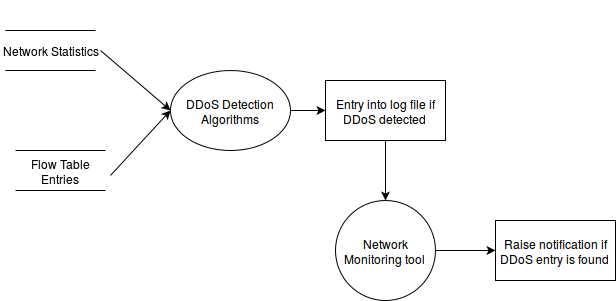
\includegraphics[scale=0.6]{dataflow0.png}
\caption{Level 0 Data Flow Diagram}
\end{center}
\end{figure}

\item
\textbf{Level 1 Data Flow Diagram :}
\newline
\begin{figure}[h]
\begin{center}
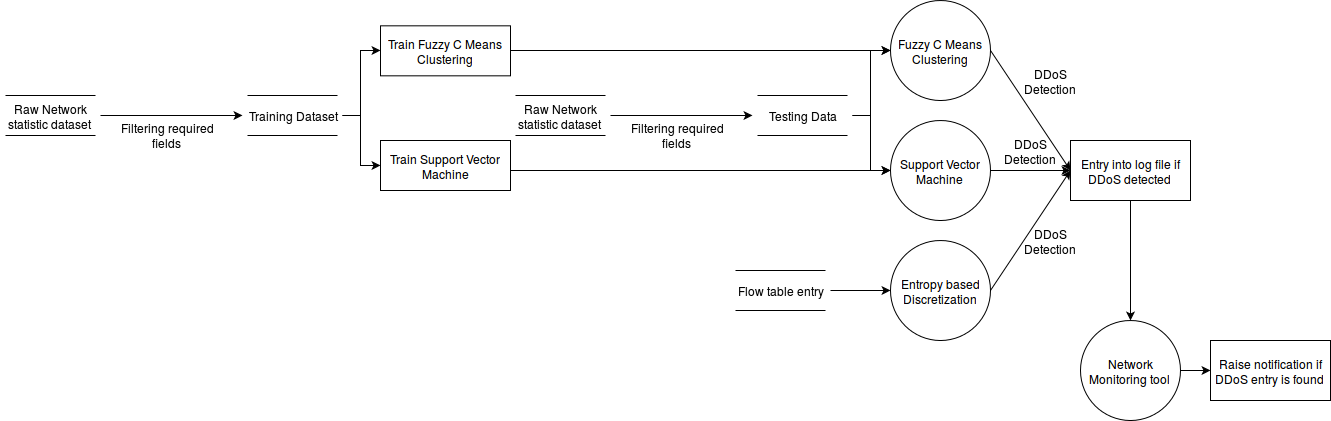
\includegraphics[scale=0.4]{dataflow1.png}
\caption{Level 1 Data Flow Diagram}
\end{center}
\end{figure}
\end{enumerate}

\newpage
\subsection{Activity Diagram}
\begin{figure}[h]
\begin{center}
\includegraphics[scale=0.5]{activity.png}
\caption{Activity Diagram}
\end{center}
\end{figure}

\subsection{Non Functional Requirements}
\begin{enumerate}
\item
\textbf{Interface Requirements}
\begin{enumerate}
\item OpenFlow Protocol :
\newline
Provides a medium for the SDN controller to direct traffic along the switches within the network.

\item Northbound API's :
\newline
Allow the SDN controller to communicate between services and applications running over the network owing to programmatic nature of SDN.

\item Southbound API's :
\newline
Allow the SDN controller to communicate between the network devices within the network.
\end{enumerate}

\item
\textbf{Software Quality Attributes}
\begin{enumerate}
\item Correctness:
\newline
The correctness of our product would depend upon the accuracy with which either of the application would detect the attack. For this purpose both applications must be trained in the network which they would monitor to generate the necessary constant values needed for their execution.

\item Availability:
\newline
As long as the network is up and running, this service would be also be available continuously monitoring the network for any anomalies.

\newpage
\item Usability: 
\newline
As and when a DDoS attack is detected, a simple notification is sent to the network administrative team. It does not disrupt their normal work flow or involve using complex application for monitoring purposes. Hence no specific training of the user is needed for using this system. 

\item Portability: 
\newline
Portability is restricted i.e. both applications must be given prior training before being deployed in a network. Thus the system being used in one enterprise cannot be used in another enterpise owing to the fact that the network traffic would vary from enterprise to enterprise such that normal traffic in one could be classified as attack traffic in another enterprise. Hence training in the network is of utmost importance.
\end{enumerate}
\end{enumerate}

\subsection{State Diagram}
\begin{figure}[h]
\begin{center}
\includegraphics[scale=0.6]{state.png}
\caption{State Diagram}
\end{center}
\end{figure}
\newpage

\AddToShipoutPictureBG*{%
\begin{tikzpicture}[overlay,remember picture]
\draw[line width=1.5pt]
    ($ (current page.north west) + (0.7cm,-0.7cm) $)
    rectangle
    ($ (current page.south east) + (-0.7cm,0.7cm) $);
\draw[line width=1.5pt]
    ($ (current page.north west) + (0.9cm,-0.9cm) $)
    rectangle
    ($ (current page.south east) + (-0.9cm,0.9cm) $);
\end{tikzpicture}
}
\chapter{Detailed Design Document}
\thispagestyle{empty}
\newpage
\section{Architectural Design}
\begin{figure}[h]
\begin{center}
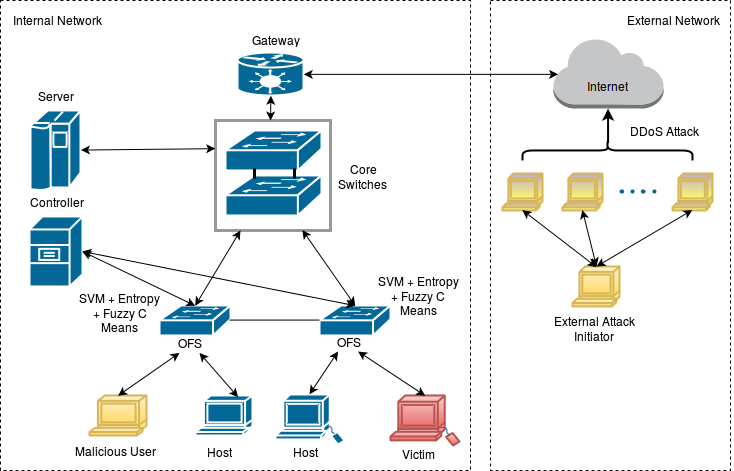
\includegraphics[scale=0.6]{architecture.png}
\caption{System Architecture}
\label{Architecture}
\end{center}
\end{figure}

During normal state of communication between two users in the network, the first packet is transmitted from the host to it's nearby switch. Initially the switch does not have any entry in its flow table as to where it should forward the incoming packet, hence the default route is to forward the packet to the controller. The controller then dictates the switch to forward the packet to the respective destination port. Along with this the controller also makes an entry in the flow table of the switch for the particular source and destination such that the future packets with the same source and destination are forwarded directly without any intervention of the controller.

This helps in reducing the time taken for communication between source and destination systems. After a particular interval of time the flow table entries are flushed and the process is repeated all over again.

The system is designed to detect two types of DDoS attacks namely :-
\begin{enumerate}
\item
Internal DDoS attack

\item
External DDoS attack
\end{enumerate}

In the first case, i.e. internal DDoS attack, the malicious user and the victim are located within the software defined network. 
whereas in external DDoS attack the host machine is from a different network. In both cases losses generated are immense.

The malicious machine can now launch attacks at two different points, one being the controller which would result in downfall of entire enterprise network incase there aren't any secondary controllers available, or the second point of attack could be one of host machines. 

In case of the attack point being the controller, the attack is generated by spoofing the source and destination ip address so that it does not match any flow table entry and hence must make a trip to the controller, this would burden the controller and thereby render its services unavailable. To overcome this issue, SVM monitors the rate of incoming packets and classifies it as normal traffic or attack traffic, similarly Entropy based mechanism would find a drop in the entropy in the network owing to the large number of same class of packets hence would be able to detect the DDoS attack, and Fuzzy C Means clustering would assign a membership value closer to "1" near the core switch since all packets are being directed towards the controller and thus would be able to detect a DDoS attack.

Another method of generating an attack would be by generating a multitude of requests at the host thereby rendering the system void of performing any other operations. This type of attack is also solved along similar guidelines such that SVM would monitor the rate of incoming packets and Entropy based mechanism would monitor the entropy of the network which would drop due to large number of same class of packets, similarly Fuzzy C Means, running on the edge switches would be able to place the incoming packets in the attack cluster thereby detecting a DDoS attack.

Hence, a comparison can be deduced as to which method would generate a result instantaneously and with higher accuracy.

Once the attack is detected by any of the applications an entry is made into the log file of the respective switch, which is constantly monitored by the network monitoring tool which on finding the entry raises a notification to the network admnistrative team. Further it is the responsibility of the network administrative team to take preventive measures to eliminate any damage that could be caused by an impending full fledged DDoS attack.

\section{Data Design}
\subsection{Dataset Description}
For the purpose of detection, all three algorithms use some form of data on which computation is performed and results are predicted. In case of Support Vector Machine the dataset consists of the network statistics, which have been converted to a "csv" file with limited fields using a terminal based tool "tshark".
\newline

The fields present in the dataset have been shown in table 2.1
\begin{table}[h]
\begin{center}
\begin{tabular}{|p{3cm}|p{3cm}|p{4cm}|p{3.5cm}|p{4cm}|}
\hline 
\textbf{Packet Interval} & \textbf{Source IP} & \textbf{Destination IP} & \textbf{Protocol} \\ 
\hline 
0.000300000 & 192.168.1.14 & 192.168.1.11 & 1 \\ 
\hline
\end{tabular} 
\end{center}
\caption{Dataset Fields - Support Vector Machine}
\end{table}

\begin{enumerate}
\item
\textbf{Packet Interval :}
\newline
Time interval between two incoming packets

\item
\textbf{Source IP :}
\newline
The source ip address of the sender machine.

\item
\textbf{Destination IP :}
\newline
The destination ip address of the receiver machine.

\item
\textbf{Protocol}
\newline
Protocol of the incoming packet.
\end{enumerate}

This dataset is again categorized into attack traffic dataset and normal traffic dataset, which can be shown in table 2.2 and 2.3, wherein the most standout variation is the packet interval field between normal traffic and attack traffic.
\begin{table}[h]
\begin{center}
\begin{tabular}{|p{3cm}|p{3cm}|p{4cm}|p{3.5cm}|p{4cm}|}
\hline 
\textbf{Packet Interval} & \textbf{Source IP} & \textbf{Destination IP} & \textbf{Protocol} \\ 
\hline 
0.000300000 & 192.168.1.14 & 192.168.1.11 & 1 \\ 
\hline
0.000100000 & 192.168.1.12 & 192.168.1.11 & 1 \\ 
\hline
0.000200000 & 192.168.1.13 & 192.168.1.11 & 6 \\ 
\hline
\end{tabular} 
\end{center}
\caption{Attack Dataset Fields - Support Vector Machine}
\end{table}

\newpage
\begin{table}[h]
\begin{center}
\begin{tabular}{|p{3cm}|p{3cm}|p{4cm}|p{3.5cm}|p{4cm}|}
\hline 
\textbf{Packet Interval} & \textbf{Source IP} & \textbf{Destination IP} & \textbf{Protocol} \\ 
\hline 
0.02000000 & 192.168.1.14 & 192.168.1.11 & 1 \\ 
\hline
0.01000000 & 192.168.1.14 & 192.168.1.11 & 1 \\ 
\hline
0.01000000 & 192.168.1.12 & 192.168.1.11 & 1 \\ 
\hline
\end{tabular} 
\end{center}
\caption{Normal Dataset Fields - Support Vector Machine}
\end{table}

Similar datasets are created during runtime using the packet capturing tool "tshark" and the classification is carried out on the same.
\newline

In case of Fuzzy C Means clustering, the nature of datasets used are the same. The only difference is the number of fields used. For Fuzzy C Means only the packet interval field is used to generate clusters and assign membership values to each packet. Also like SVM, Fuzzy C Means uses two datasets i.e. attack traffic and normal traffic for training the model, using the packet capturing tool "tshark", again which is stored in a csv file format. The training dataset appears to be like the one showed in table 2.4 and 2.5

\begin{table}[h]
\begin{center}
\begin{tabular}{|p{3cm}|}
\hline 
\textbf{Packet Interval} \\ 
\hline 
0.000300000 \\ 
\hline
0.000100000 \\ 
\hline
0.000200000 \\ 
\hline
\end{tabular} 
\end{center}
\caption{Attack Dataset Fields - Fuzzy C Means clustering}

\begin{center}
\begin{tabular}{|p{3cm}|}
\hline 
\textbf{Packet Interval} \\ 
\hline 
0.02000000 \\ 
\hline
0.01000000 \\ 
\hline
0.01000000 \\ 
\hline
\end{tabular} 
\end{center}
\caption{Normal Dataset Fields -Fuzzy C Means clustering}
\end{table}

However, unlike SVM and Fuzzy C Means that use packet level statistics for classification and clustering, Entropy based discretization uses the flow table entries residing in the switch to perform its computation. The flow table entries are dumped into a file during each time interval, which is then looked up by the entropy based application to detect what is the entropy of the network and accordingly detect whether a DDoS attack has been launched or not.
\newline

\newpage
Sample flow entry :
\newline
$cookie=0x0, duration=240.478s, table=0, n\_packets=21975265, n\_bytes=2153575970, idle\_timeout=60, idle\_age=0, priority=65535,icmp,in\_port=2,vlan\_tci=0x0000,dl\_src=4a:06:64:e9:ef:f0,dl_dst=f2:57:bd:4c:19:28,nw\_src=10.0.0.2,nw\_dst=10.0.0.1,nw\_tos=0,icmp\_type=0,icmp\_code=0 actions=output:1$
\newline

wherein the fields used during processing are:
\begin{enumerate}
\item
\textbf{$n\_packets$ :}
\newline
The total number of packets transitted by the switch having the same flow details.

\item
\textbf{$protocol$ :}
\newline
The protocol of the incoming packets.

\item
\textbf{$nw\_src$ :}
\newline
Source IP address

\item
\textbf{$nw\_dst$ :}
\newline
Destination IP address
\end{enumerate}
\newpage

\AddToShipoutPictureBG*{%
\begin{tikzpicture}[overlay,remember picture]
\draw[line width=1.5pt]
    ($ (current page.north west) + (0.7cm,-0.7cm) $)
    rectangle
    ($ (current page.south east) + (-0.7cm,0.7cm) $);
\draw[line width=1.5pt]
    ($ (current page.north west) + (0.9cm,-0.9cm) $)
    rectangle
    ($ (current page.south east) + (-0.9cm,0.9cm) $);
\end{tikzpicture}
}
\chapter{Project Implementation}
\thispagestyle{empty}
\newpage

\section{Introduction}
There was always an option to implement the project by creating a Software Defined Network in a  single system using network simulator called Mininet. But doing this would have decreased the quality of the project and our commitment that the solution can be used in real world deployment. In order to validate the effectiveness of the solution in real time environment we decided to deploy our own Software Defined Network on a small scale. This deployment was a challenge in itself as it is a new technology which is not well matured.

\section{Methodologies}
\begin{algorithm}
\caption{Entropy Based Discretization}
\begin{algorithmic}[1]

\Function{Collect\_Flow}{}

\State Collect the flows from switch and store it in a text file.

\State Read this text file line by line and for every line do,

\State Seperate $dest\_ip$ and $no\_of\_packet$

\State Calculate total number of packets for every $dest\_ip$ in current interval.

\EndFunction

\Function{Calc\_Entropy}{}'

\State First, calculate the probabilily using,
$P_{i} = \frac{X_{i}}{\sum_{i=1}^{N} X_{i}} $
\newline
\hspace*{1cm}
where, 
\newline
\hspace*{1cm}
$P_{i} = $Probability of $i^{th} dest\_ip $
\newline
\hspace*{1cm}
$X_{i} = $Packet count on $i^{th} dest\_ip$
\newline
\hspace*{1cm}
$N = $Total number of $ dest\_ip$

\State Now, Calculate entropy of network using, 
$H(S_{j}) = -\sum_{i=1}^{N} p_{i} log p_{i} $
\newline
\hspace*{1cm}
where, 
\newline
\hspace*{1cm}
$H(S_{j}) = $Entropy of $j^{th} $ switch

\State Calculate the difference between above calculated entropy value and normal entropy value and stored it in $diff$

\EndFunction

\Function{ddos\_detection}{}

\State Compare the above calculated $diff$ with predefined $threshold$ value.

\If{$diff > threshold$}
\State Increment $ddos\_detected\_count$ 

	\If {$ ddos\_detected\_count > min\_ddos\_detected $ in perticular window}
        \State \textbf{Generate alert of DDoS attack}
    \EndIf

\Else
\State Increment program counter.

\EndIf

\EndFunction


\end{algorithmic}
\end{algorithm}

\begin{algorithm}
\caption{Support Vector Machine}
\begin{algorithmic}[1]

\Function{Predict}{$features, w, b$}
\State $classification \leftarrow \textbf{sign}(\textbf{dot}(features,w)) + b)$
\State \Return $classification$
\EndFunction

\Function{Train}{$Data$}
\State $optimized\_sv \leftarrow \textbf{dict()}$
%\State $all\_data = [\ ]$
\For{$y_i $ in $data$}
	\For{$featureset$ in $data[y_i]$}
		\For{$feature$ in $featureset$}
			\State all\_data.\textbf{append}($feature$)
			\Comment{$all\_data$ is a list}
		\EndFor
	\EndFor
\EndFor
%\State $max\_feature\_value \leftarrow \textbf{max}(all\_data)$
%\State $min\_feature\_value \leftarrow \textbf{min}(all\_data)$
\State $all\_data \leftarrow \textbf{None}$
\State $step\_size \leftarrow [\textbf{max}(all\_data)*0.1]$
\State $b\_range\_multiple, b\_multiple \leftarrow 2, 5$
\State $latest\_optimum \leftarrow \textbf{max}(all\_data) * 10$ 
\State $range\_value \leftarrow \textbf{max}(all\_data) * b\_range\_multiple$
\For{$step$ in $step\_size$}
	\State $w \leftarrow [latest\_optimum,latest\_optimum]$ 
	\State $optimized \leftarrow \textbf{False}$
	\While{$\textbf{not}$ $optimized$}
		\For{$b$ \textbf{in range}($-range\_value, range\_value, step*b\_multiple$) }
	
			\For{$transformation\ \textbf{in}\ transforms$}
				\State $w\_t \leftarrow w * transformation		$	
				\State $found\_option \leftarrow \textbf{True}$
				\For{$i\ \textbf{in}\ data$}
					\For{$x_i\ \textbf{in}\ data[i]$}
						\State $y_i \leftarrow I$ 		
						\If{$\textbf{not}\ y_i*(\textbf{dot}(w_t,x_i) + b \geq 1)$}
						\State $found\_option \leftarrow \textbf{False}$
						\EndIf
									
					\EndFor
				\EndFor			
				\If {$found\_option$}
					\State \textbf{normalize}($optimized\_sv[w\_t]$) $\leftarrow [w_t, b]$ 			 	
				\EndIf			
			\EndFor		
	
	\EndFor
	\If {$w[0] < 0$}
		\State $optimized \leftarrow \textbf{True}$	
	\Else
		\State $w \leftarrow w - step$
	\EndIf
	\EndWhile
	\State $norms \leftarrow \textbf{sort}(optimized\_sv)$
	\State $w \leftarrow optimized\_sv[norms[0]][0]$
	\State $b \leftarrow optimized\_sv[norms[0]][1]$
	\State $final\_optimum \leftarrow optimized\_sv[norms[0]][0]$
\EndFor
	
\EndFunction
\end{algorithmic}
\end{algorithm}


\begin{algorithm}
\caption{Fuzzy C Means Clustering}
\begin{algorithmic}[1]
\Function{Calculate\_membership}{$cluster\_count, centroids, dataset$}
\State $membership[i,j] \leftarrow \frac{\frac{-2}{d_{ij}^{m-1}}}{\sum_{i=1}^{c}{{d_{ij}^{m-1}}}}$
\newline
\hspace*{1cm}
where, 
\newline
\hspace*{1cm}
$m = Fuzzifier (default\ 2)$
\newline
\hspace*{1cm}
$c = cluster\ count$
\newline
\hspace*{1cm}
$i = centroid\ point, j = data\ point$
\newline
\hspace*{1cm}
$d = euclidean\ distance\ between\ i\ and\ j$
\State \Return $membership$
\EndFunction

\Function{Calculate\_centroid}{$cluster\_count, centroids, dataset$}
\State $centroid_{i} \leftarrow \frac{\sum_{j=1}^{n}u_{ij}^{m}X_{ij}}{\sum_{n}^{j=1}u_{ij}^{m}}$
\newline
\hspace*{1cm}
where, 
\newline
\hspace*{1cm}
$m = Fuzzifier (default\ 2)$
\newline
\hspace*{1cm}
$c = cluster\ count$
\newline
\hspace*{1cm}
$u = membership$
\newline
\hspace*{1cm}
$i = centroid\ point, j = data\ point$
\newline
\hspace*{1cm}
$d = euclidean\ distance\ between\ i\ and\ j$
\State $centroids = [ centroid_1, \ldots, centroid_c ]$
\State \Return $centroids$
\EndFunction

\Function{Fuzzy}{$cluster\_count, centroids, training\_dataset$}
\State Let, $normal\_centroids[]$, $attack\_centroids[]$ be 1-dimensional lists and,
\State $ membership $ be a 2-dimensional list of order n x c
\newline
\hspace*{1cm}
where, 
\newline
\hspace*{1cm}
n $=$ number of data points
\newline
\hspace*{1cm}
c $=$ number of centroids
\State $ membership\_df $ be a dataframe representing the 2-dimensional $membership$ list
\State $training\_data \leftarrow dataframe\ for\ training\ data $
\State $membership \leftarrow calculate\_membership(cluster\_count, centroids, training\_data)$
\State $centroid \leftarrow calculate\_centroid(cluster\_count, centroids, training\_data)$

\While{True}
\State $old\_membership \leftarrow membership$
\State $old\_membership\_df \leftarrow membership\_df$
\State $membership \leftarrow calculate\_membership(cluster\_count, centroids, training\_data)$
\If {$old\_membership == membership$}
\State \textbf{break}
\EndIf
\EndWhile

\State Identify \textbf{attack clusters}.
\State $min\_membership \leftarrow$ minimum membership in attack clutser.

\While{True}
\State Capture packets during runtime.
\State $testing\_data \leftarrow dataframe\ for\ testing\ data$
\State $membership \leftarrow calculate\_membership(cluster\_count, centroids, testing\_data)$
\State $attack\_packets \leftarrow $ Total packets having membership value above $min\_membership$ value.
\If {$attack\_packets \geq threshold * total\_packets$}
\State \Return DDoS
\EndIf
\EndWhile
\EndFunction
\end{algorithmic}
\end{algorithm}

\begin{minipage}{\textwidth}
\end{minipage}

\newpage
\AddToShipoutPictureBG*{%
\begin{tikzpicture}[overlay,remember picture]
\draw[line width=1.5pt]
    ($ (current page.north west) + (0.7cm,-0.7cm) $)
    rectangle
    ($ (current page.south east) + (-0.7cm,0.7cm) $);
\draw[line width=1.5pt]
    ($ (current page.north west) + (0.9cm,-0.9cm) $)
    rectangle
    ($ (current page.south east) + (-0.9cm,0.9cm) $);
\end{tikzpicture}
}
\chapter{Software Testing}
\thispagestyle{empty}
\newpage


\section{Type of Testing Used}
\begin{itemize}
\item Unit Testing
\item Integration Testing
\item System Testing
\item Positive Testing
\item Negative Testing
\end{itemize}


\section{Test Cases and Test Results}

\begin{enumerate}
\item\begin{flushleft}
Unit Testing 
\end{flushleft} 
	\begin{tabular}{|p{1cm}|p{3cm}|p{2.6cm}|p{2.5cm}|p{2.5cm}|}
	\hline 
	\textbf{Unit} & \textbf{Description} & \textbf{Scenario} & \textbf{Expected Output} & 		\textbf{Generated Output}\\ 
	\hline
	
	SVM & Attack Traffic & Attack has occured & Alert generation & Alert Generated\\
	\hline
	
	SVM & Normal Network Traffic & SDN functioning in normal mode & No alert generation & Alert is not Generated \\
	\hline
	
	EBD & Attack Traffic & Attack has occured & Alert generation & Alert Generated\\
	\hline
	
	EBD & Normal Network Traffic & SDN functioning in normal mode & No alert generation & Alert is not Generated \\
	\hline
	
	FCM & Attack Traffic & Attack has occured & Alert generation & Alert Generated\\
	\hline
	
	FCM & Normal Network Traffic & SDN functioning in normal mode & No alert generation & Alert is not Generated \\
	\hline
	
	\end{tabular}
	\linebreak
	
\item \begin{flushleft}
Integration Testing 
\end{flushleft} 
	\begin{tabular}{|p{3.5cm}|p{2.9cm}|p{2.5cm}|p{2.5cm}|}
	\hline 
	\textbf{Description} & \textbf{Scenario} & \textbf{Expected Output} & \textbf{Generated 		Output}\\ 
	\hline

	All three algorithms are running simultaneously and attack traffic in the network & Attack has occured & Alert generation & Alert Generated\\
	\hline
	
	All three algorithms are running simultaneously and Normal traffic in the network & SDN functioning in normal mode & no alert generation & Alert is not Generated\\
	\hline
	
	\end{tabular}
	\linebreak
\newpage	
\item \begin{flushleft}
System Testing 
\end{flushleft} 
	\begin{tabular}{|p{3.5cm}|p{2.9cm}|p{2.5cm}|p{2.5cm}|}
	\hline 
	\textbf{Description} & \textbf{Scenario} & \textbf{Expected Output} & \textbf{Generated 		Output}\\ 
	\hline
	
	Time span between attack detection and alert generation & Attack has occured & Instantaneous alert generation & Alert generated within 1 sec.\\
	\hline
	
	Normal Network Traffic & SDN functioning in normal mode & No alert generation & Alert is not Generated\\
	\hline
	
	\end{tabular}
	
	
\item \begin{flushleft}
Positive Testing 
\end{flushleft} 
	\begin{tabular}{|p{3.5cm}|p{2.9cm}|p{2.5cm}|p{2.5cm}|}
	\hline 
	\textbf{Description} & \textbf{Scenario} & \textbf{Expected Output} & \textbf{Generated 		Output}\\ 
	\hline
	
	Attack Traffic & Attack has occured & Alert generation & Alert Generated\\
	\hline
	
	\end{tabular}
	\linebreak
	
\item \begin{flushleft}
Negative Testing 
\end{flushleft} 
	\begin{tabular}{|p{3.5cm}|p{2.9cm}|p{2.5cm}|p{2.5cm}|}
	\hline 
	\textbf{Description} & \textbf{Scenario} & \textbf{Expected Output} & \textbf{Generated 		Output}\\ 
	\hline
	
	 Normal Network Traffic & SDN functioning in normal mode & No alert generation & Alert is not Generated \\
	 \hline	
	
	\end{tabular}

\end{enumerate}


\newpage

\AddToShipoutPictureBG*{%
\begin{tikzpicture}[overlay,remember picture]
\draw[line width=1.5pt]
    ($ (current page.north west) + (0.7cm,-0.7cm) $)
    rectangle
    ($ (current page.south east) + (-0.7cm,0.7cm) $);
\draw[line width=1.5pt]
    ($ (current page.north west) + (0.9cm,-0.9cm) $)
    rectangle
    ($ (current page.south east) + (-0.9cm,0.9cm) $);
\end{tikzpicture}
}
\chapter{Results}
\thispagestyle{empty}
\newpage
\section{Screenshots}
\begin{figure}[h]
\centering
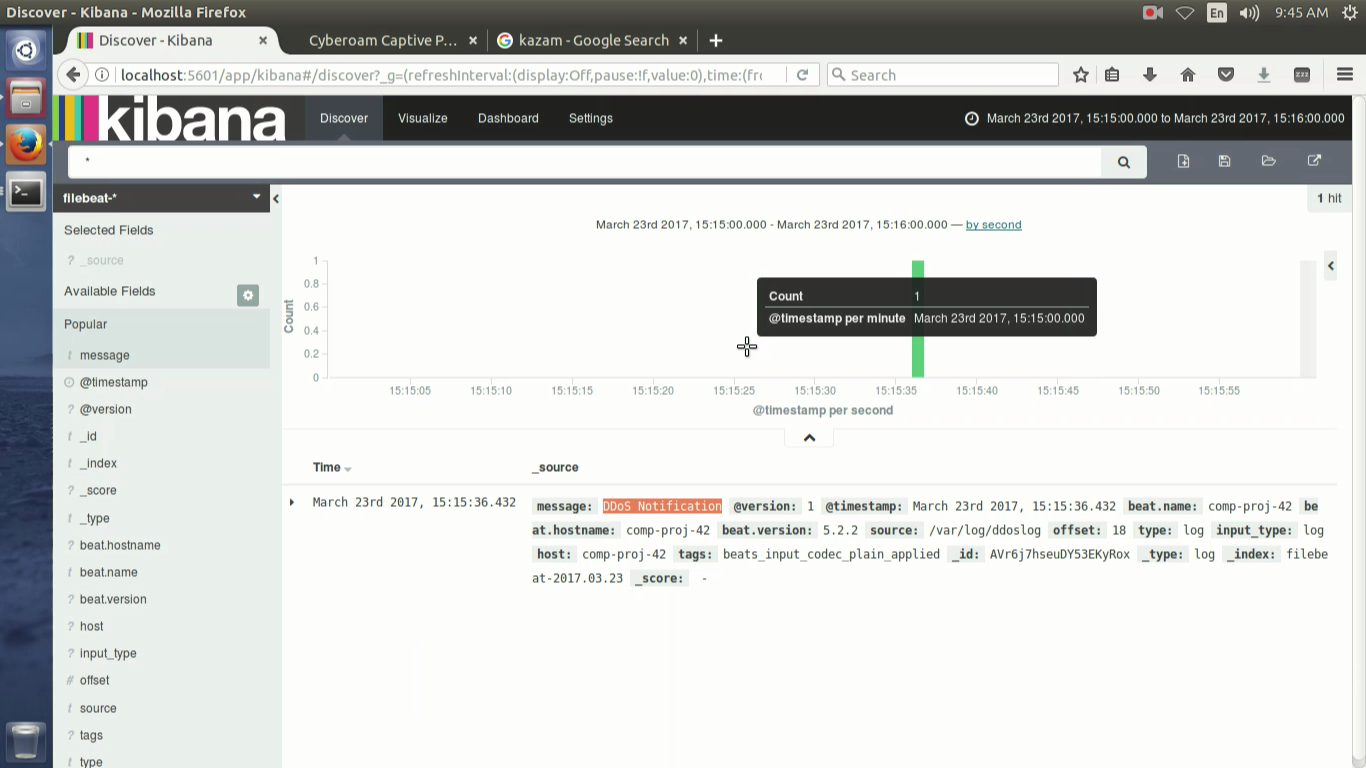
\includegraphics[scale=0.3]{Kibana.png}
\caption{Kibana Dashboard}
\end{figure}

\begin{figure}[h]
\centering
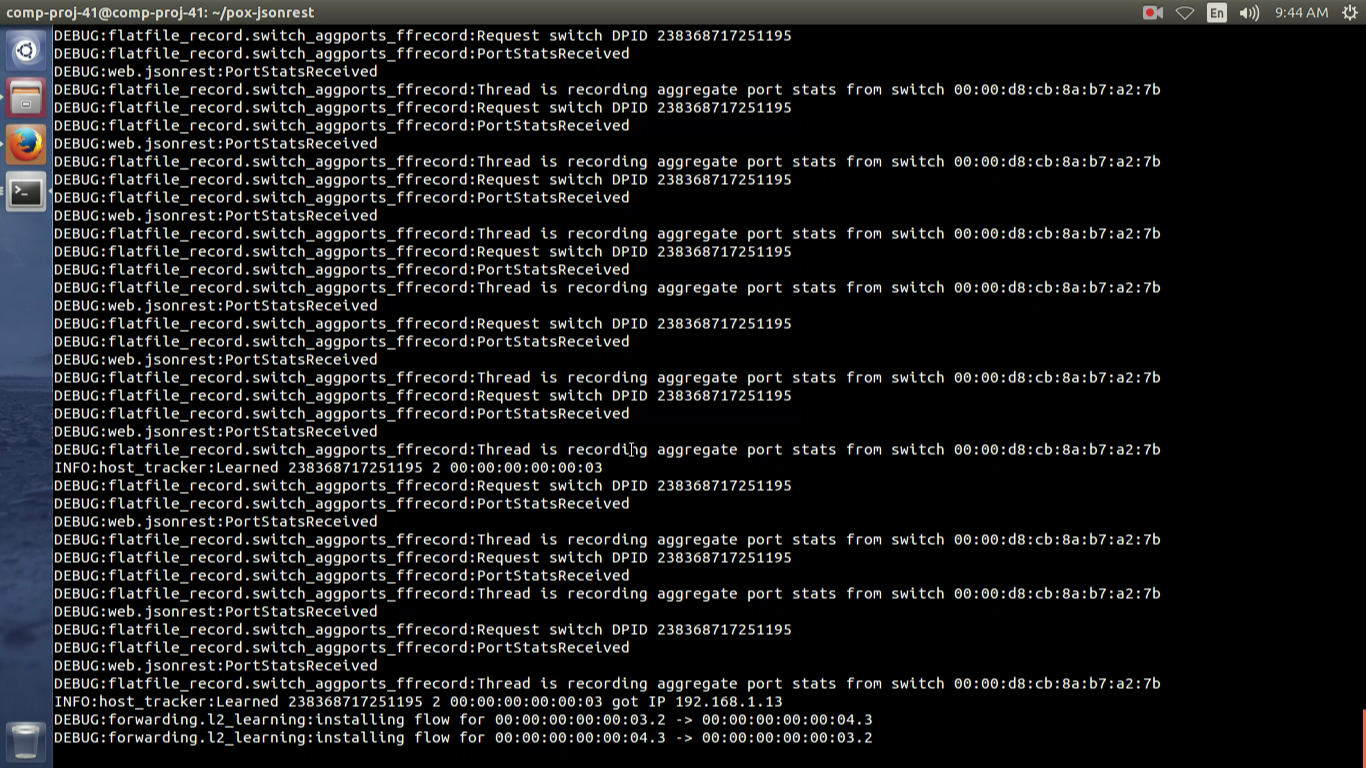
\includegraphics[scale=0.3]{Controller.png}
\caption{POX Controller Output}
\end{figure}

\newpage

\section{Output}

\begin{figure}[h]
\centering
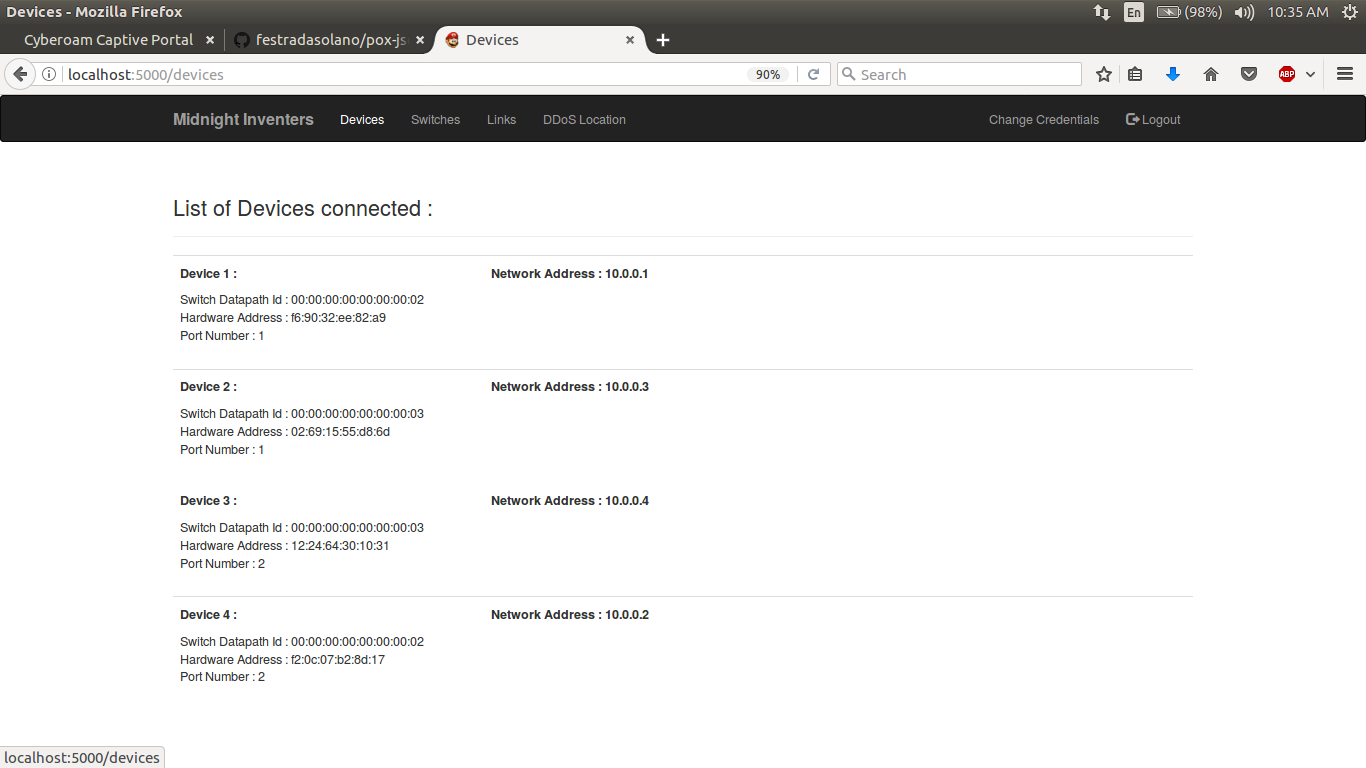
\includegraphics[scale=0.3]{devices.png}
\caption{Flask - List of Devices}
\end{figure}

\begin{figure}[h]
\centering
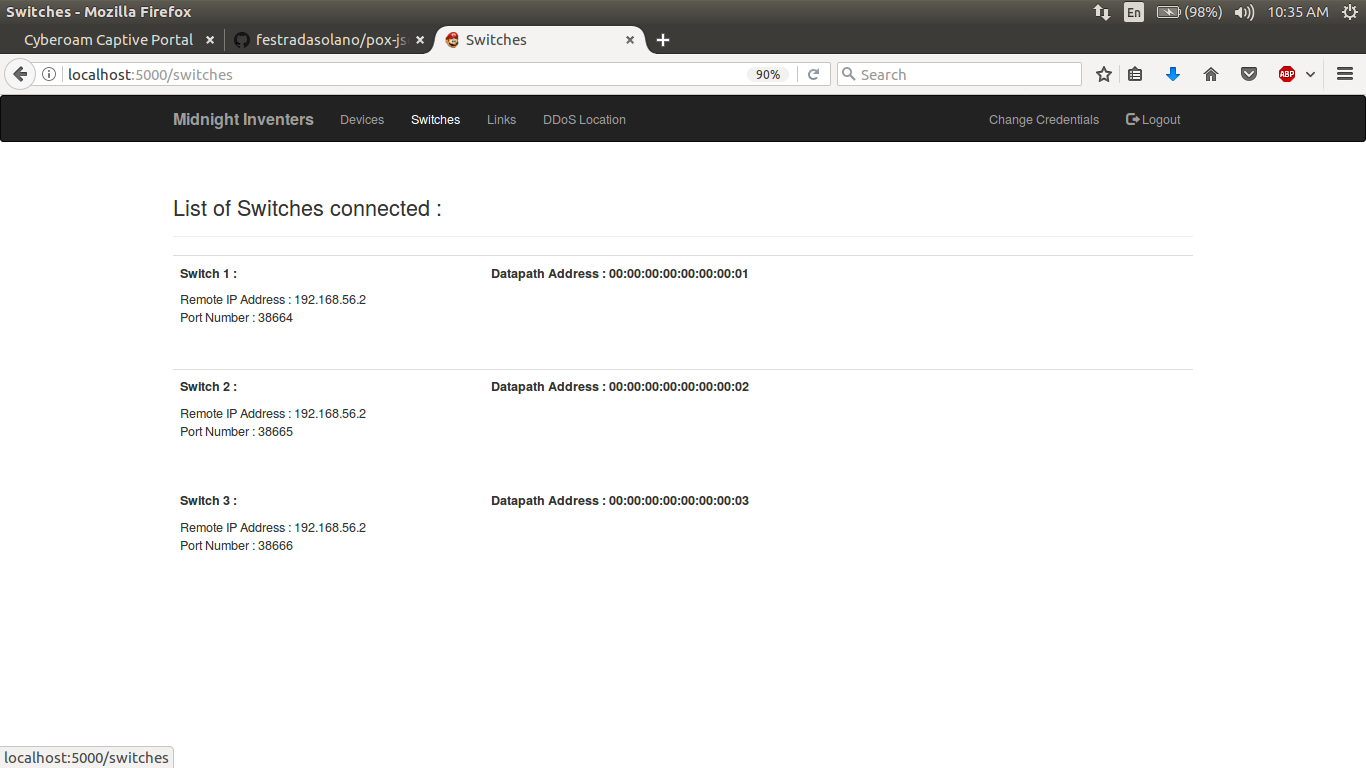
\includegraphics[scale=0.3]{switches.png}
\caption{Flask - List of Switches}
\end{figure}

\newpage

\begin{figure}[h]
\centering
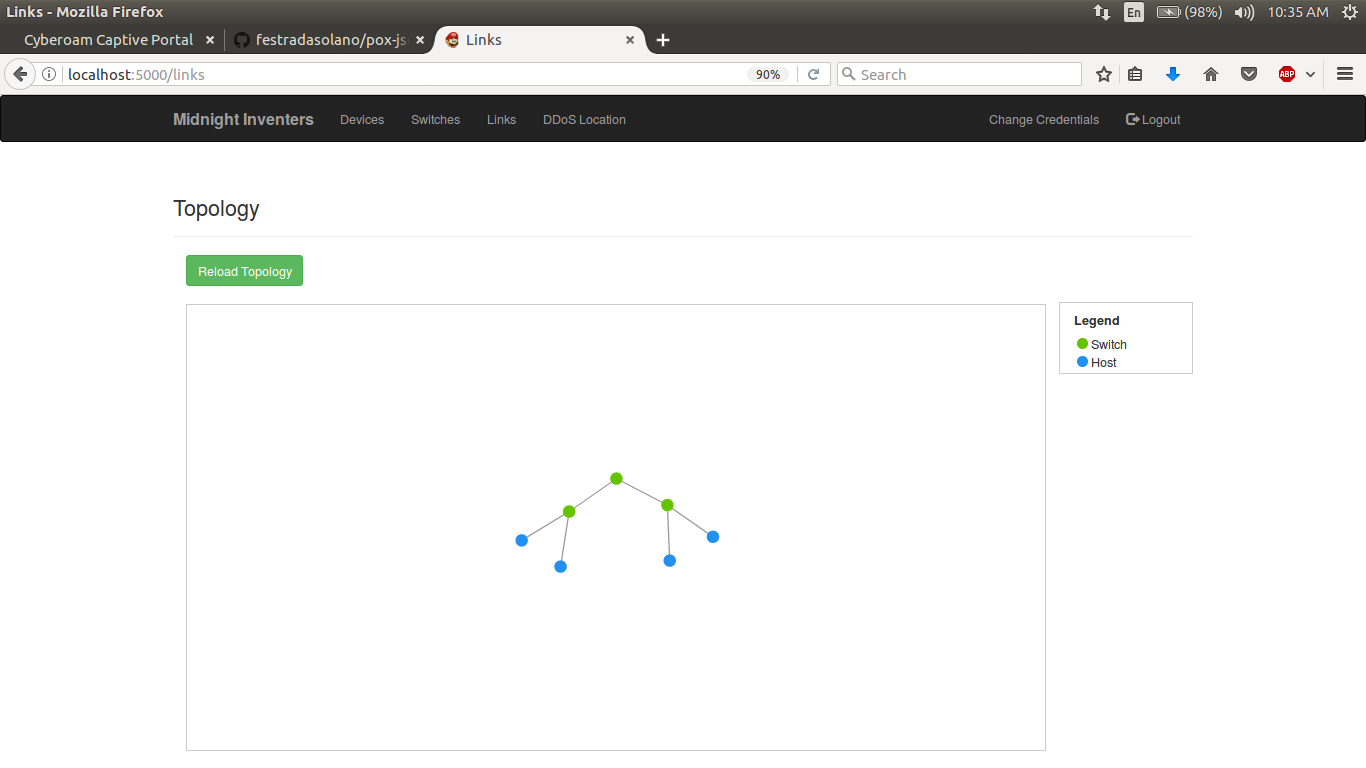
\includegraphics[scale=0.3]{flask.png}
\caption{Flask - SDN Topology}
\end{figure}


\begin{figure}[h]
\centering
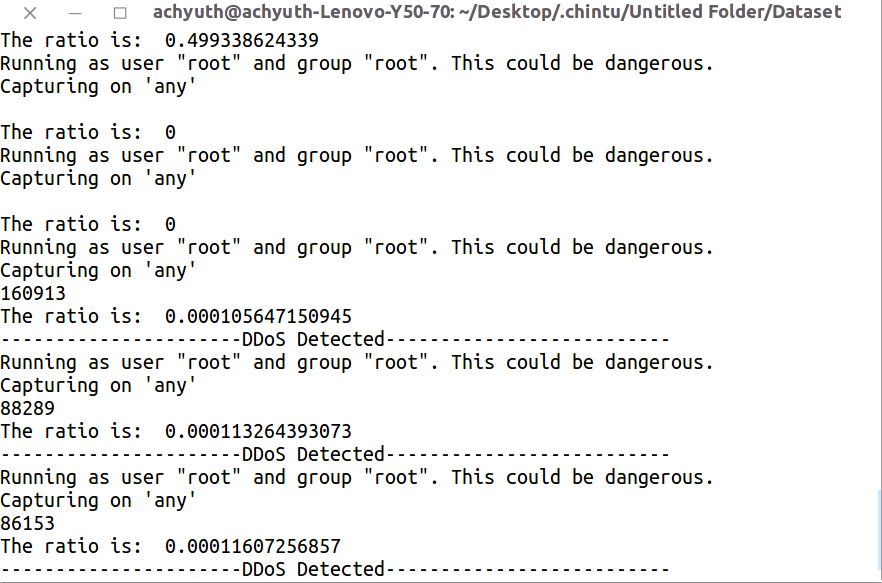
\includegraphics[scale=0.4]{SVMOutput.png}
\caption{SVM Algorithm Output}
\end{figure}


\begin{figure}
\centering
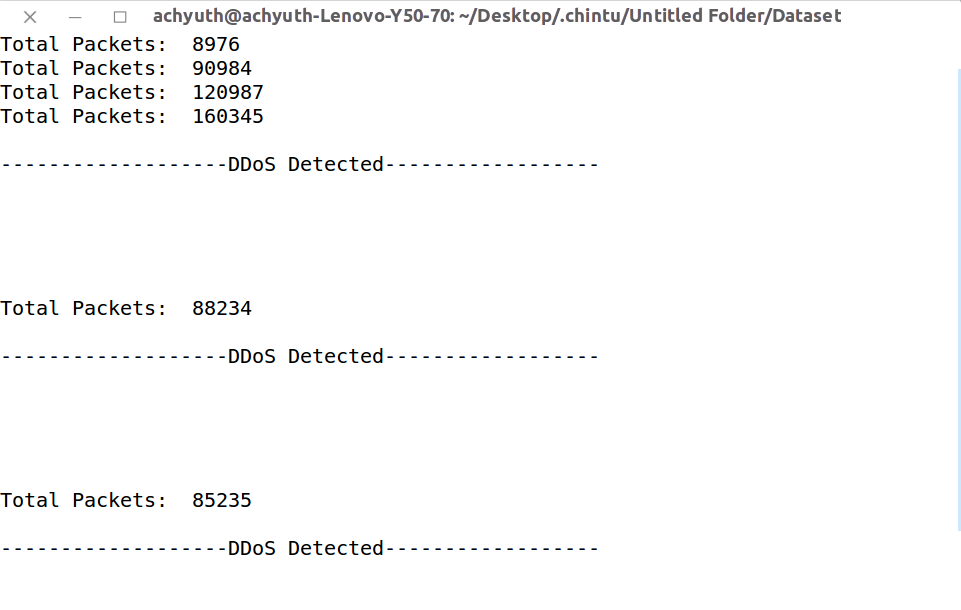
\includegraphics[scale=0.4]{EBDOutput.png}
\caption{Entropy Based Discretization Algorithm Output}
\end{figure}


\begin{figure}
\centering
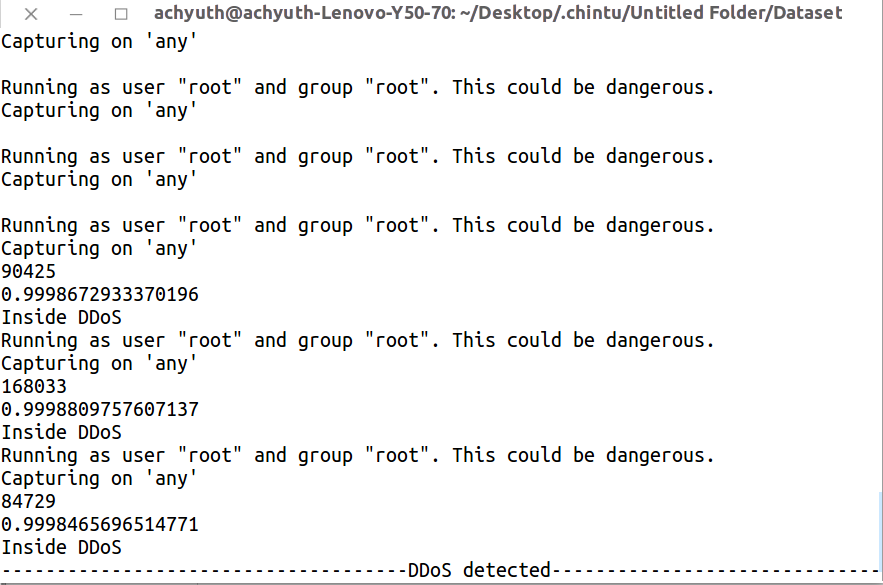
\includegraphics[scale=0.4]{FuzzyOutput.png}
\caption{Fuzzy C-Means Algorithm Output}
\end{figure}

\newpage
\AddToShipoutPictureBG*{%
\begin{tikzpicture}[overlay,remember picture]
\draw[line width=1.5pt]
    ($ (current page.north west) + (0.7cm,-0.7cm) $)
    rectangle
    ($ (current page.south east) + (-0.7cm,0.7cm) $);
\draw[line width=1.5pt]
    ($ (current page.north west) + (0.9cm,-0.9cm) $)
    rectangle
    ($ (current page.south east) + (-0.9cm,0.9cm) $);
\end{tikzpicture}
}
\chapter{Deployment and Maintenance}
\thispagestyle{empty}
\newpage
\section{Installation and un-installation}
\subsection{Installation}
Given the required hardware is present along with root priveleges (sudo) the following softwares can be installed. We illustrate the installation procedure considering Ubuntu 14.04 is installed, however any Linux Operating System will work well with little changes in the procedure.

According to the Software Requirements the installation procedure is as follows:
\begin{enumerate}
\item
Oracle VirtualBox
\newline
It can either be installed from the software center of Ubuntu or more advanced users can install it from the command line.
\newline
Step 1: Go to the Ubuntu Software Center and search for VirtualBox
\newline
Step 2: Click on Install and provide the password

\item
Open vSwitch
\newline
You can install it from the command line for Ubuntu 14.04. However if you prefer the latest version which is not updated in its repository, you can install from tar file
\begin{center}
\$ sudo apt-get install openvswitch-switch
\end{center}

\item
tshark
\newline
If you simply need tshark then it can be installed using the following command. If you need Wireshark then tshark will be installed along with it by default.
\begin{center}
\$ sudo apt-get install tshark
\end{center}

\item
Ubuntu VM's
\newline
After VirtualBox or any hypervisor is available you need to install 4 virtual machines ech having at least 1 logical core, 1.5 GB RAM and 10 GB minimum hard disk. 

For VirtualBox select the downloaed ISO of Ubuntu 14.04 along with the suitable VM specifications to install them.

\item
Apache Web Server
\newline
After the VM's have been installed install the Apache web server using simple command.
\begin{center}
\$ sudo apt-get install apache2
\end{center}

\item
Ostinato
\newline
This is an open source packet generation tool which can be installed using
\begin{center}
\$ sudo apt-get install ostinato
\end{center}

\item
Elasticsearch
\begin{center}
\$ sudo apt-get install elasticsearch 
\end{center}

\item
Logstash
\begin{center}
\$ sudo apt-get install logstash
\end{center}

\item
Kibana
\begin{center}
\$ sudo apt-get install kibana
\end{center}

\item
hsflowd
\newline
Download the debian file for hsflowd from the official site. For any further queries read the documentation. This need to be installed on both the physical machines.
\begin{center}
\$ sudo dpkg -i hsflowd.deb
\end{center}

\item
sFlow-RT
\newline
Download the sflow-rt application from the official site. You just need to run the main program of sflow-rt.

\item
POX
\newline
Download the POX controller from the GitHub repo which also includes the json-rest  part integrated with it. You just need to enter the directory and run the controller using the pox.py program.

\item
Python Flask
\newline
You will need python pip for installing Flask. Install pip using
\begin{center}
\$ sudo apt-get install python-pip \\
\$ sudo pip install Flask
\end{center}

\item
Filebeat Agent
\newline
Install the filebeat agent for tailing the log file and sending to the elasticsearch server
\begin{center}
\$ sudo apt-get install filebeat
\end{center}

\item
Watcher
\newline
This is available as a plugin for elasticsearch. Refer elasticsearch documentation for installing watcher plugin.
\end{enumerate}

\subsection{Uninstallation}
Remove the VM's from VirtualBox and free the used space
For all other softwares a simple purge command will work well.
\begin{center}
\$ sudo apt-get purge --remove $<$name\_of\_software$>$
\end{center}
\newpage

\AddToShipoutPictureBG*{%
\begin{tikzpicture}[overlay,remember picture]
\draw[line width=1.5pt]
    ($ (current page.north west) + (0.7cm,-0.7cm) $)
    rectangle
    ($ (current page.south east) + (-0.7cm,0.7cm) $);
\draw[line width=1.5pt]
    ($ (current page.north west) + (0.9cm,-0.9cm) $)
    rectangle
    ($ (current page.south east) + (-0.9cm,0.9cm) $);
\end{tikzpicture}
}
\chapter{Conclusion and Future Scope}
\thispagestyle{empty}
\newpage
The report introduces the problems faced in the Software Defined Networking Environment such as DDoS,
application layer attack, brute force and phishing. As the SDN Controller seperates the Application layer and 
the Data flow plane in the network, it becomes a point of vulnerability for the attackers to target by using 
such attacks.

DDoS attack when targetted on the controller can pose a huge impact on the whole network compromizing the system 
responsible for the Business logic. Thus it is very important to use a mechanism which can detect and mitigate such 
anomaly based attacks, we focus on the prior and not the later part of the mechanism.

There are several methods which can be used for the detection of DDoS such as use of neural networks, chaotic 
systems, filtering algorithms etc. Considering the advantages of Support Vector Machines, Entropy Based Discretization and Fuzzy C Means Clustering algorithms, we will be using them.

We then procede by stating the product features,user characteristics, system features, interfaces and quality 
attributes like correctness,usability etc. We also provide necessary diagramatic representations like the 
sequence diagram, use case diagram etc.

We then give a description of the system components, system architecture as well as the functioning of the whole
network environment. We also specify two cases of the DDoS attack scenarios namely, internal and external attacks and the method in which we detect the attack using the proposed algorithmic strategies. After the detection of the attack, the network administrator will be notified by the mechanism and a graphical interface would be provided for the administrator for finding the point of attack.

%This project will be a step towards solving the security issues faced right now. This will be a challenging endevour for us as we try to incorporate concepts like networking, machine learning and data mining.  

The current implementation of our project does not include the mitigation of DDoS attacks due to the chances of false positives being generated, this would  result in blocking out legitimate users which will seriously impact the organization. So, the future scope of our project includes developing a module for mitigation, increasing the accuracy of the system to remove false positives.


\newpage

\AddToShipoutPictureBG*{%
\begin{tikzpicture}[overlay,remember picture]
\draw[line width=1.5pt]
    ($ (current page.north west) + (0.7cm,-0.7cm) $)
    rectangle
    ($ (current page.south east) + (-0.7cm,0.7cm) $);
\draw[line width=1.5pt]
    ($ (current page.north west) + (0.9cm,-0.9cm) $)
    rectangle
    ($ (current page.south east) + (-0.9cm,0.9cm) $);
\end{tikzpicture}
}
\SkipTocEntry\chapter{Bibliography}
\thispagestyle{empty}
\newpage
\begingroup
\renewcommand{\chapter}[2]{}
\begin{thebibliography}{9}
\bibitem{BasePaper1}
Diego Kreutz, Fernando M. V. Ramos, Paulo Verissimo, Christian Esteve Rothenberg, Siamak Azodolmolky, Steve Uhlig,
``Software-Defined Networking: A Comprehensive Survey",
Version 2.01,
8 Oct 2014

\bibitem{BasePaper2}
Open Networking Foundation, 
``Software-Defined Networking: The New Norm for Networks",
ONF white paper, 
April 13, 2012

\bibitem{BasePaper3}
Shiva Rowshanrad, Sahar Namvarasl, Vajihe Abdi, Maryam Hajizadeh, Manijeh Keshtgary,
``A survey on SDN, the future of networking",
in Journal of Advanced Computer Science and Technology,
pg 232-248,
2014

\bibitem{BasePaper4}
Rishikesh Sahay, Gregory Blanc, Zonghua Zhang, Herve Debar,
``Towards Autonomic DDoS Mitigation using Software Defined Networking",
Feb 2015,
http://www.internetsociety.org/doc/towards-autonomic-DDoS-mitigation-using-software-defined-networking

\bibitem{BasePaper5}
Seyed Mohammad Mousavi,
``Early Detection of DDoS Attacks in Software Defined Networks Controller",
2014

\bibitem{BasePaper6}
Shunsuke Oshima, Takuo Nakashima, Toshinori Sueyoshi,
``Early DoS/DDoS Detection Method using Short-term Statistics",
Presented at International Conference on Complex, Intelligent and Software Intensive Systems,
2010

\bibitem{BasePaper7} 
Kokila RT, S.Thamarai Selvi, Kannan Govindarajan,
``DDoS Detection and Analysis in SDN-based Environment Using Support Vector Machine Classifier",
presented at Sixth International Conference on Advanced Computing(ICoAC),
2014,

\bibitem{BasePaper8}
Xue Li, Dongming Yuan, Hefei Hu, Jing Ran, Shulan Li, 
``DDoS detection in SDN switches using support vector machine classifier",
in Joint International Mechanical, Electronic and Information Technology Conference, 
2015

\bibitem{BasePaper9} 
Rui Wang, Zhiping Jia∗, Lei Ju,
``An Entropy-Based Distributed DDoS Detection Mechanism in Software-Defined Networking",
in IEEE Trustcom/BigDataSE/ISPA,
DOI 10.1109/Trustcom.2015.389,
2015

\bibitem{BasePaper10}
T.Subbulakshmi, Dr. S. Mercy Shalinie, V.GanapathiSubramanian, K.BalaKrishnan, D. AnandKumar, K.Kannathal,
``Detection of DDoS Attacks using Enhanced Support Vector Machines with Real Time Generated Dataset",
in IEEE-ICoAC, 
2011

\bibitem{BasePaper11}
I Gde Dharma N., M. Fiqri Muthohar, Alvin Prayuda J. D., Priagung K., Deokjai Choi,
``Time-based DDoS Detection and Mitigation for SDN Controller",
Presented at APNOMS,
2015

\bibitem{BasePaper12}
Shibo Luo, Jun Wu, Jianhua Li,
``A Defense Mechanism for Distributed Denial of Service Attack in Software-Defined Networks",
Presented at Ninth International Conference on Frontier of Computer Science and Technology,
2015

\bibitem{BasePaper13}
K. Giotis, C. Argyropoulos, G. Androulidakis, D. Kalogeras, V. Maglaris,
``Combining OpenFlow and sFlow for an effective and scalable anomaly detection and mitigation mechanism on SDN environments",
2013, 
http://dx.doi.org/10.1016/j.bjp.2013.10.014

\bibitem{BasePaper14}
Seyed Mohammad Mousavi, Marc St-Hilaire,
``Early Detection of DDoS Attacks against SDN Controllers",
Presented at International Conference on Computing, Networking and Communications, Communications and Information Security
Symposium,
2015

\bibitem{BasePaper15}
P. K. Agrawal, B. B. Gupta, Satbir Jain,
``SVM Based scheme for Predicting Number of Zombies in a DDoS Attack",
Presented at European Intelligence and Security Informatics Conference,
2011

\bibitem{BasePaper16}
A. Ramamoorthi, T. Subbulakshmi, Dr. S. Mercy Shalinie,
``Real Time Detection and Classification of DDoS Attacks using Enhanced SVM with String Kernels",
in IEEE-International Conference on Recent Trends in Information Technology,
ICRTIT 2011,
June 2011

\bibitem{BasePaper17}
Ingo Steinwart, Andreas Christmann,
``Support Vector Machines",
Springer, 
2008

\bibitem{BasePaper18}
Alexander Gelbukh, Félix Castro Espinoza, Sofía N. Galicia-Haro,
``Nature-Inspired Computation and Machine Learning",
Springer,
2014

\bibitem{BasePaper19}
Vapnik, Vladimir,
``The Nature of Statistical Learning Theory",
Springer,
2000

\bibitem{BasePaper20}
Jose Valente de Oliveira, Witold Pedrycz,
``Advances in Fuzzy Clustering an its Applcations",
Wiley,
2007

\bibitem{BasePaper21}
Sindhu Arumugam, Dr. V Vanitha, Ms. V.P. Sumathi,
``Detection of BotNet using Fuzzy C-Means Clustering by Analysing the network traffic",
International Journal of Scientific \& Engineering Research, Vol. 6 Issue 4,
April 2015

\bibitem{BasePaper22}
Disha Sharma, 
``Fuzzy Clustering as an Intrusion Detection Technique",
International Journal of Computer Science \& Communication Network, Vol. 1(1),
September-October 2011

\bibitem{BasePaper23}
Jerzy W. Grzymala Busse, 
``Discretization Based on Entropy \& Multiple Scanning", 
Entropy,
2013.

\bibitem{BasePaper24}
Claudio Rebelo De Sa, Carlos Soares, Arno Knobbe , 
``Entropy Based Discretization methods for ranking data", 
Elsevier Vol. 329.

\bibitem{BasePaper25}
Jiawei Han, Micheline Kamber, Jian Pei, 
``Data Mining: Conepts and Techniques 3rd ed.", 
Morgan Kaufmann, 
July 2011.

\bibitem{BasePaper26}
Kevin Meurer, 
``A Simple Guide to Entropy-Based Discretization", 
URL: http://kevinmeurer.com/a-simple-guide-to-entropy-based-discretization/
\end{thebibliography}
\endgroup
\newpage

\AddToShipoutPictureBG*{%
\begin{tikzpicture}[overlay,remember picture]
\draw[line width=1.5pt]
    ($ (current page.north west) + (0.7cm,-0.7cm) $)
    rectangle
    ($ (current page.south east) + (-0.7cm,0.7cm) $);
\draw[line width=1.5pt]
    ($ (current page.north west) + (0.9cm,-0.9cm) $)
    rectangle
    ($ (current page.south east) + (-0.9cm,0.9cm) $);
\end{tikzpicture}
}
\SkipTocEntry\chapter{Annexure A}
\thispagestyle{empty}
\newpage
\SkipTocEntry\section{IDEA Matrix}
\begin{table}[h]
\caption{IDEA Matrix}

\begin{center}
\begin{tabular}{|>{\bf}M{2.5cm}||>{\bf}M{2.5cm}||>{\bf}M{2.5cm}||>{\bf}M{2.5cm}|}
\hline
\rowcolor{lightgray}
I & D & E & A \\ \hline
\normalfont{Innovative} & \normalfont{Detect}  & \normalfont{Evaluate} & \normalfont{Associate} \\ \hline
\normalfont{Increase} & \normalfont{Decrease}  & \normalfont{Effective} & \normalfont{Acquire} \\ \hline
\normalfont{Investment} & \normalfont{Depict}  & \normalfont{Enhance} & \normalfont{Analyse} \\ \hline
\end{tabular}
\end{center}
\end{table}

\begin{center}
\begin{tabular}{|m{2cm}|m{7cm}|}
\hline
Innovative & Up till now, DDoS detection systems uses a single mechanism for its working. Here, the system will be using two mechanisms i.e. support vector machine, fuzzy c means clustering and entropy based discretization simultaneously which is \textbf{innovative}. \\

&\\

Increase & As the system will be using support vector machine, fuzzy c means clustering and entropy based discretization, efficiency of the system will \textbf{increase}. \\

&\\

Investment & As the system contains Software components only. So, \textbf{zero investment} is required to implement the system in already deployed software defined network. \\

\hline
\end{tabular}
\end{center}

\vspace*{1cm}
\begin{center}
\begin{tabular}{|m{2cm}|m{7cm}|}
\hline

Detect & The system will \textbf{detect} DDoS attack and raise notification to the network administrator team. \\

&\\

Decrease & The DDoS detection algorithm will \textbf{decrease} the possibility of false positive attack detection. \\

&\\

Depict & The system will \textbf{depict} appropriately whether the network traffic is normal or attack traffic. \\

\hline
\end{tabular}
\end{center}

\newpage
\begin{center}
\begin{tabular}{|m{2cm}|m{7cm}|}
\hline

Evaluate & An important part of the implementation is the \textbf{evaluation} of the rate of flow of packets per unit time. \\

&\\

Effective & The system analyses the traffic and detects the attack at runtime thus, increasing the \textbf{effectiveness}. \\

&\\

Enhance & The accuracy of the system will be \textbf{enhanced} by using an environment - specific training dataset for SVM and Fuzzy C Means. \\

\hline
\end{tabular}
\end{center}

\vspace*{1cm}
\begin{center}
\begin{tabular}{|m{2cm}|m{7cm}|}
\hline

Associate & The project is a step towards \textbf{association} and integration of next generation networking with advanced computing concepts like Machine Learning and Data Mining. \\

&\\

Acquire & The flow table containing the flow entries along with the information of the count of the packets is \textbf{acquired} from the SDN switches. \\

&\\

Analyse & The system will \textbf{analyse} the data acquired from the switches to perform the intended task of detecting the DDoS attack. \\

\hline
\end{tabular}
\end{center}
\newpage
\SkipTocEntry\section{Mathematical Model}
\SkipTocEntry\subsection{Mathematical Model}
{\setlength{\mathindent}{0cm}
\begin{equation}
S = \lbrace \lbrace I \rbrace ,\lbrace P \rbrace,\lbrace O \rbrace \rbrace
\end{equation}

\noindent
where,\\
$I =$ Input set,\\
$P = \lbrace P_{EBD}, P_{SVM}, P_{FCM} \rbrace$ Processing set, \\
$O =$ Output set

\SkipTocEntry\subsection{Input:}
{\setlength{\mathindent}{0cm}
\begin{equation}
I = \lbrace N \rbrace
\end{equation}

\noindent
where,\\
$N = \lbrace $ Network Statistics $ \rbrace $, \\
$F =\lbrace F_{i} \mid F_{i} \in T , \forall i$ $ F_{i} =$ Individual entry $ \rbrace$, \\
$T = \lbrace $ Flow Table $ \rbrace$, \\
$F \subseteq N$

\SkipTocEntry\subsection{Input for EBD:}

{\setlength{\mathindent}{0cm}
\begin{equation}
I_{EBD} = \lbrace U_{i} \mid U_{i} = ($ Source Address, Destination Address, Port no., Count$),  $ $ U_{i}  \subset F_{i} \rbrace
\end{equation}

\SkipTocEntry\subsection{Input for SVM:}

{\setlength{\mathindent}{0cm}
\begin{equation}
I_{SVM} = \lbrace V_{i} \mid V_{i} = ($ Source Address, Destination Address, Port no., Time, Protocol, Count$),  $ $ V_{i}  \subset F_{i} \rbrace
\end{equation}

\SkipTocEntry\subsection{Input for FCM:}

{\setlength{\mathindent}{0cm}
\begin{equation}
I_{FCM} = \lbrace V_{i} \mid V_{i} = ($Time$),  $ $ V_{i}  \subset F_{i} \rbrace
\end{equation}



\SkipTocEntry\subsection{Processing:}
$P_{EBD} $ $ (I_{EBD},$ $O_{EBD})$\\
$\lbrace$

\begin{enumerate}

\item 
{\setlength{\mathindent}{0cm}}
\begin{equation}
P_{i} = \frac{C_{i}}{N}
\end{equation}
where, \\ $c =$ counter, \\ $N = \sum_{i=0}^{n} C_{i}$, \\ $n =$ no. of entries.

\item 
{\setlength{\mathindent}{0cm}}
\begin{equation}
\varepsilon = \sum_{i=0}^{n} - P_{i} log P_{i}
\end{equation}

\newpage
\item 
\begin{equation}
(\lambda < \varepsilon) \rightarrow (\beta = 0)
\end{equation}
\begin{equation}
(\lambda > \varepsilon) \rightarrow (\beta = 1)
\end{equation}

\item  
\begin{equation}
O_{EBD} = \lbrace \beta \mid \beta \in (0,1) \rbrace
\end{equation}

\end{enumerate}

\noindent
$\rbrace$
\\


\noindent
$P_{SVM} $ $ (I_{SVM},$ $O_{SVM})$\\
$\lbrace$
\indent
Here, \\
\indent $\gamma$ , $c$, $x$, $x_{1}$, $x_{2}$, $b$ and $\overline{\omega}$ are constants.\\
\indent These values are calculated from Training Phase.\\
\indent Training of SVM is based on dataset used.


\begin{enumerate}

\item 
\begin{equation}
RBF = e^{-\gamma(\mid x_{1}-x_{2} \mid)+c}
\end{equation}
where, \\ $\gamma =$ width of boundries of hyperplane, \\ $c =$ soft margin parameter, \\ $x_{1}, $ $x_{2} =$ support vectors.


\item
\begin{equation}
y = \overline{\omega} * x + b
\end{equation}
where, \\ $x =$ support vector, \\ $b =$ boundary width, \\ $\overline{\omega} =$ libsvm.w().

\item
\begin{equation}
(y \leq -1) \rightarrow (\alpha = 1)
\end{equation}
\begin{equation}
(y \geq 1) \rightarrow (\alpha = 0)
\end{equation}

\item
\begin{equation}
O_{SVM} = \lbrace \alpha \mid \alpha \in (0, 1) \rbrace
\end{equation}

\end{enumerate}

$\\ \rbrace$

\newpage

\noindent
$P_{FCM} $ $ (I_{FCM},$ $O_{FCM})$\\
$\lbrace$
\indent
Here, \\
\indent $m$ is a constant.\\
\indent This value is used for the calculation of the membership values of the data points.\\


\begin{enumerate}

\item 
\begin{equation}
u_{ij} = \frac{\frac{-2}{d_{ij}^{m-1}}}{\sum_{i=1}^{c}{{d_{ij}^{m-1}}}}
\end{equation}
where, \\ $d_{ij}^{m-1}=$ distance of the $i^{th}$ point from the $j^{th}$ centroid\\
$c =$ centroid.

\item
\begin{equation}
C_{i} = \frac{\sum_{j=1}^{n}u_{ij}^{m}X_{ij}}{\sum_{n}^{j=1}u_{ij}^{m}}
\end{equation}
where, \\ $u_{ij}^{m}=$ membership value of the data point. \\
$X_{ij}=$ data point. 


\item
\begin{equation}
(X \geq \lambda) \rightarrow (w = 1)
\end{equation}
\begin{equation}
(X < \lambda) \rightarrow (w = 0)
\end{equation}


\item
\begin{equation}
O_{FCM} = \lbrace w \mid w \in (0, 1) \rbrace
\end{equation}

\end{enumerate}

$\\ \rbrace$




\SkipTocEntry\subsection{Output:}

\begin{equation}
O_{EBD} = \lbrace z \mid \exists z, z \in \beta \rbrace
\end{equation}
\begin{equation}
O_{SVM} = \lbrace x \mid \exists x, x \in \alpha \rbrace
\end{equation}
\begin{equation}
O_{FCM} = \{w \mid \exists w, w\in \gamma \rbrace
\end{equation}


\begin{equation}
O_{system} = \lbrace O_{EBD} \cup O_{SVM} \cup O_{FCM} \rbrace
\end{equation}

\SkipTocEntry\subsection{Feasibility Study}
To check the feasibility of Entropy Based Discretization, Support Vector Machine abd Fuzzy C-Means Clustering:
\newline Since, the problem we solve is essentially a decision problem, it is very essential to analyse the running time of the system. The strategies used in the system are SVM, Entropy Based Discretization and Fuzzy C-Means clustering. It is well known that EBD takes O(n) running time thus is in P.\\
\newline
Now, we will find the computational complexity for Support Vector Machines:\\
For a training dataset D=\{$x_i$,$y_i$\} where, $x_i$ $\in$ $\Re$ and $y_i$ $\in$ \{+1,-1\}.\\
The Support Vector Machine classifies with seperating hyperplane given by:\\

\begin{equation}
D(x)=w^Tx+b
\end{equation}

The above equation is obtained by:
\begin{equation}
L=\frac{1}{2} \emph{w}^2 - \sum_{}^{} \zeta_i
\end{equation}

s.t. $y_i$($w^T$ $x_i$ + b) $\geq$ 1 - $\zeta_i$, $\zeta_i$ $>$ 0 for i=1,2,...,m \\
\newline The problem is equivalent to the problem:\\
\begin{equation}
Max L(\alpha)= \sum_{i=1}^{M} \alpha_i - \frac{1}{2} \sum_{i=1}^{m}\sum_{j=1}^{m} y_iy_j\alpha_i\alpha_jk(x_i,y_j)
\end{equation}

where k($x_1$,$y_1$) is the Mercer's Kernel which is used for the 
Dimensional reduction.\\
\newline We will use the following four steps to prove the complexity of the SVM problem:
\begin{enumerate}
\item
Denote the problem as \textbf{$\pi$} and justify that it is in NP.
\item
Selecting a known problem \textbf{$\pi$'} which is in NP.
\item
Construct a tranformation function from $\pi$' to $\pi$.
\item
Prove that the transformation function is polynomial.
\end{enumerate}
\begin{itemize}

\item
\textbf{The SVM Problem ($\pi$)}
\newline For a set of kernels A=\{$k_1,k_2,...,k_n$\} the objective function can be written as:\\

\begin{equation}
C(A')=	\Big[\sum_{k \in A'}^{}\Big(\frac{1}{q}\Big[\sum_{i=1}^{m} \alpha_i - \frac{1}{2q^2} \sum_{i=1}^{m}\sum_{j=1}^{m}y_iy_jk(x_i,x_j)\alpha_i\alpha_j\Big]\Big)^2- B\Big]^2
\end{equation}	
\newline 

Where, we have to find a subset A' $\subseteq$ A of size q to minimize the cost. The cost function is used for reaching a bound B using set of Kernels, dataset and the Support Vectors.\\
\item
\textbf{SVM is in NP}
\newline To justify that SVM is in NP, we have to show that any instance of the problem can be guessed and verified to solve or not in polynomial time.\\
Let there be a function, that accepts q which returns random indices of q from the set of kernels and computes the most optimum solution A'. As the set of Lagrange Multipliers, dataset, q and Bound is known beforehand, the kernel evaluations are the only states.  These kernel evaluations are merely dot products among the directional vectors. The evaluation is polynomial and thus the instances A' can easily be generated and verified. Hence, we can say that SVM is in NP.
\item
\textbf{Selecting a known NP-Complete Problem ($\pi$')}
\newline The known problem selected is the subset problem which is as defined,\\
Given a set A, a size s(a) for each a $\in$ A and an integer B. Is there an A' $\subseteq$ A such that the sum of the sizes of the elements in is exactly B?\\
\item
\textbf{Transformation function $\mathcal{F}$ from $\pi$' to $\pi$}
\newline The transformation function $\mathcal{F}$ should map every instance (\emph{I}) such that every instance of "yes" in $\pi$ should map to the corresponding instance (\emph{I'}) in $\pi$'.\\
First, A stands for set of kernels: A=\{$A_1,A_2,...,A_n$\} \\
To compute B the following procedure should be followed: \\
\begin{enumerate}
\item
Solve SVM for all k $\in$ A with dataset D.
\item
Use the kernel $k^*$ and the dataset D to find the most optimal solution for SVM denoted by $M^* = (V^*,k^*)$
\item 
Now, B can be calculated by:- 
\begin{equation}
B = \Big[\sum_{i=1}^{m} \alpha_i - \frac{1}{2}\sum_{i=1}^{m}\sum_{j=1}^{m}y_iy_jk^*(x_i,x_j)\alpha_i,\alpha_j\Big]^2
\end{equation} 
\item
Finally we have to calculate the size function s(a)=s(k $\in$ A) which can be done by the formula:- \\
\begin{equation}
s(k) = \Big[\big(\frac{1}{q}\sum_{i=1}^{m}\alpha_i - \frac{1}{2q^2}\sum_{i=1}^{m}\sum_{j=1}^{m}y_iy_jk(x_i,x_j)\alpha_i\alpha_j\Big)\Big]^2
\end{equation}
Where, s(k) is the value of the objective function. 
\end{enumerate} 
Now, we know that $\sum_{k \in A}^{}s(k)=B$ when $k^*(x_i,x_j)=\frac{1}{q^2}\sum_{k \in A'}^{},(k_i,k_j)$ \\
This can be written in the form: \\
\begin{equation}
\Big[\sum_{k \in A'}^{}\Big(\frac{1}{q}\sum_{i=1}^{m}\alpha_i - \frac{1}{2q^2}\sum_{i=1}^{m}\sum_{j=1}^{m}y_iy_jk(x_i,x_j)\alpha_i\alpha_j\Big) \Big]^2 = \Big[\sum_{i=1}^{m} \alpha_i - \frac{1}{2}\sum_{i=1}^{m}\sum_{j=1}^{m}y_iy_jk^*(x_i,x_j)\alpha_i\alpha_j\Big]^2
\end{equation}
Taking squared-root and using summation property, \\
\begin{equation}
\sum_{k \in A'}\Big(\frac{1}{q}\sum_{i=1}^{m}\alpha_i\Big)+\sum_{k \in A'}^{}\Big[-\frac{1}{2q^2}\sum_{i=1}^{m}\sum_{j=1}^{m}y_iy_jk(x_i,x_j)\alpha_i\alpha_j\Big] = \sum_{i=1}^{m}\alpha_i-\frac{1}{2}\sum_{i=1}^{m}\sum_{j=1}^{m}y_iy_jk^*(x_i,x_j)\alpha_i\alpha_j
\end{equation}
Simplifying the equation,
\begin{equation}
\sum_{k \in A'}\Big[\frac{1}{q^2}\sum_{i=1}^{m}\sum_{j=1}^{m}y_iy_jk(x_i,x_j)\alpha_i\alpha_j\Big] = \sum_{i=1}^{m}\sum_{j=1}^{m}y_iy_jk^*(x_i,x_j)\alpha_i\alpha_j
\end{equation}
Substituting $\Delta_{i,j}$ = $y_iy_j\alpha_i\alpha_j$ for simplification purpose \\
\begin{equation}
\sum_{k \in A'}\Big[\frac{1}{q^2}\sum_{i=1}^{m}\sum_{j=1}^{m}\Delta_{i,j}k(x_i,x_j)\Big] = \sum_{i=1}^{m}\sum_{j=1}^{m}\Delta_{i,j}k^*(x_i,x_j)
\end{equation}
Cancelling common terms,
\begin{equation}
\frac{1}{q^2}\sum_{k \in A'}{}k(x_i,x_j)=k^*(x_i,x_j)
\end{equation}
Thus, 
\begin{equation}
\sum_{k \in A'}s(k) = B \leftrightarrow k^*(x_i,x_j) = \frac{1}{q^2}\sum_{k \in A'}k(x_i,x_j)
\end{equation}
This implies that the transformed subset problem is equivalent to SVM classification using an optimum kernel. Thus, for every instance of (\emph{I')} if the answer is "yes" the answer can be mapped for the instance  of (\emph{I}). \\
\item
\textbf{$\mathcal{F}$ is a polynomial Transformation}
\newline The last part is to prove that the $\mathcal{F}$ is polynomial. The most expensive step is to find the Boundary (B) in the training phase.\\
This problem of training is a quadratic problem(QP). This problem can be seen as a convex problem. There are methods like Ellipsoids to solve it in polynomial time. 
It is also known that QP can be solved in O($m^3$), for  SVM ``m'' is the number of input vectors. Therefore, $\mathcal{F}$ is a polynomial transformation. \\
\newline 

Now, we have to analyze the Fuzzy C-Means clustering.\\
the following are: the steps of the running of the FCM algorithm:
\begin{enumerate}
\item
Initializing the centroids for the cluster.
\item
Calculate the membership values of the data points for the initialized clusters.
\item
recalculate the centroids of the cluster.
\item
recalculate the membership values for every data point until the centroid values and the membership values do not change.
\end{enumerate}

The calculation of the membership values take place using the following equation:- 
\begin{equation}
u_{ij} = \frac{\frac{-2}{d_{ij}^{m-1}}}{\sum_{i=1}^{c}{{d_{ij}^{m-1}}}}
\end{equation}
And, the calculation of the centroid is done by the following equation:- 
\begin{equation}
C_{i} = \frac{\sum_{j=1}^{n}u_{ij}^{m}X_{ij}}{\sum_{n}^{j=1}u_{ij}^{m}}
\end{equation}

\newpage
\begin{enumerate}
\item
Fuzzy C-Means is a generalization of Hard C-Means or K-Means clustering algorithm. The clustering based algorithms are well known to fall under the NP-Hard type of problems.
\item
This is because, the clustering algorithms provide a global solution which causes them not to converge even for a large number of iterations. Thus, we have to limit the number of iterations that can take place.\\
\item
Also, there is no linear relationship between the point of convergence and the number of iterations. Therefore, we can not be certain that for a particular number of iterations the clustering will converge. This is analogous to the Halting probelm in the Turing machine which is well known to be a NP-Hard problem.
\item
The time complexity of FCM is O(nd$c^{2}$i) where, \\
n = Number of data points. \\
c = Number of clusters. \\
d = Number of dimensions. \\
i = Number of iterations. \\
\end{enumerate}
Thus, \\
SVM is NP-Complete, Entropy based mechanism is Polynomial and Fuzzy C-Means clustering is NP-Hard.\\
By Cook's Theorem, P $\in$ NP therefore, the proposed solution is NP-Hard. 
\end{itemize}
\newpage

\AddToShipoutPictureBG*{%
\begin{tikzpicture}[overlay,remember picture]
\draw[line width=1.5pt]
    ($ (current page.north west) + (0.7cm,-0.7cm) $)
    rectangle
    ($ (current page.south east) + (-0.7cm,0.7cm) $);
\draw[line width=1.5pt]
    ($ (current page.north west) + (0.9cm,-0.9cm) $)
    rectangle
    ($ (current page.south east) + (-0.9cm,0.9cm) $);
\end{tikzpicture}
}
\SkipTocEntry\chapter{Annexure B}
\thispagestyle{empty}
\newpage
\SkipTocEntry\section{Distributed Computation}
The controller in an Software Defined Network is the centralized entity, which is responsible for the interfacing between Application layer and the underlying network hardware. Since, the controller imposes the application logic onto the datapath of the SDN. This requires a lot of computation. \\

	Furthermore, during the scenario of a DDoS attack there is an excruciating load on the network and especially the SDN controller.	Thus, is unwise to run an application on top of the controller as it can cause an overhead on the system. We exploit the dormant processing power of the SDN switches to our advantage by using them as computational nodes. Our DDoS detection mechanism will work on the switches distributed throughout the network. \\

Each switch will scan its underlying traffic. The advantages of this are twofold firstly, there will not be an overhead on the remaining network and secondly, it will be easier for the network administrator for finding the origin of the DDoS attack vastly reducing the cost and effort for the recovery. \\

Thus, we divide the whole network traffic statistics into several concurrent switches for the computation making it a divide and conquer strategy.

\SkipTocEntry\section{Functional Dependancies}
There are mainly Five Functions in the system namely,
\begin{enumerate}
\item
A function which will continuously send the formatted traffic statistics which can be accepted by the Support Vector Machine, Entropy Based Descretization mechanism and Fuzzy C-Means Clustering.
\item
A Function for the Support Vector Machine classifier which will classify the traffic into normal or attack traffic and update the log files if attack traffic is detected.
\item
A Function for the Entropy Based Discretization Mechanism which will compare the flow of traffic with the threshold value and update the log files if the rate of flow of packets exceeds the threshold.
\item
A Function for the Fuzzy C-Means Clustering algorithm which will cluster the incomming packets time difference betwwen two consecutive packets.
\item
A Function which will monitor the log files to check whether there is an attack scenario or not.
\end{enumerate}
The algorithms depend on the real-time input of the Network statistics, the function responsible for monitoring is dependent on the SVM, Entropy mechanism and Fuzzy Clustering. Thus, there is a one-many-one mapping between this function.
\begin{center}
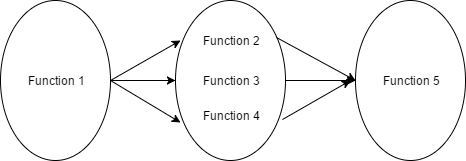
\includegraphics[scale=0.5]{functionalDependency.png}
\end{center}
\newpage

\SkipTocEntry\section{UML Diagrams}
\begin{figure}[h]
\begin{center}
\includegraphics[scale=0.5]{use_case.png}
\caption{Use Case Diagram}
\vspace{2cm}

\includegraphics[scale=0.5]{state.png}
\caption{State Diagram}
\end{center}
\end{figure}

\begin{figure}
\begin{center}
\includegraphics[scale=0.5]{activity.png}
\caption{Activity Diagram}

\vspace{1cm}
\includegraphics[scale=0.5]{sequence.png}
\caption{Sequence Diagram}
\end{center}
\end{figure}

\begin{figure}
\begin{center}
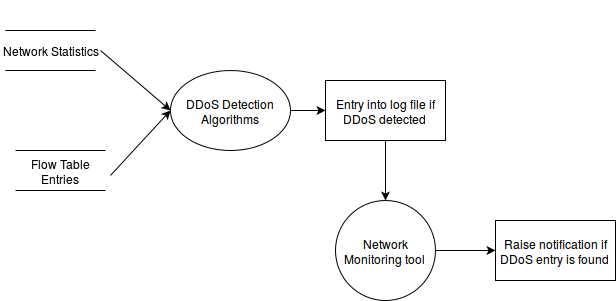
\includegraphics[scale=0.5]{dataflow0.png}
\caption{Dataflow Level 0 Diagram}

\vspace{3cm}
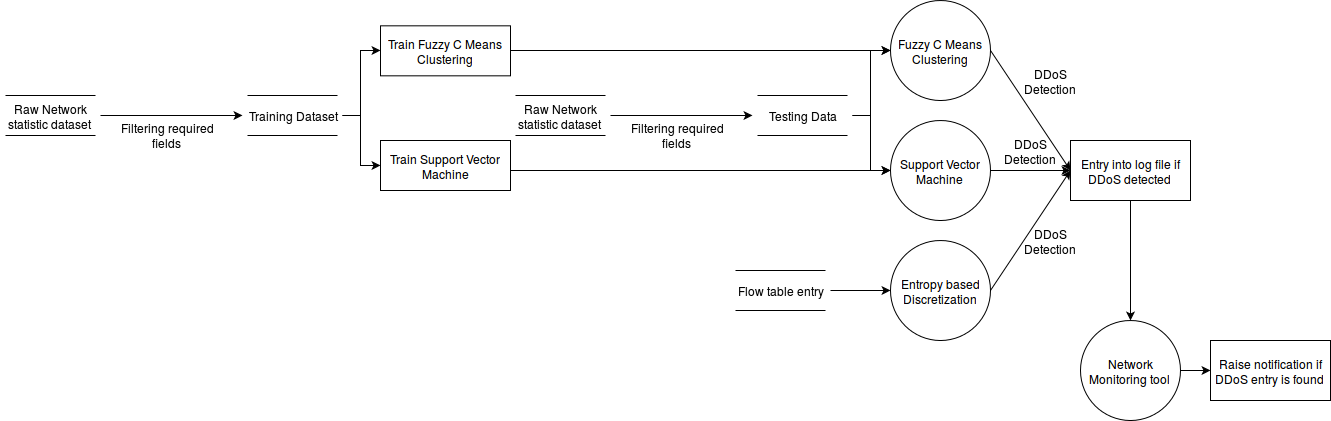
\includegraphics[scale=0.4]{dataflow1.png}
\caption{Dataflow Level 1 Diagram}
\end{center}
\end{figure}
\newpage

\AddToShipoutPictureBG*{%
\begin{tikzpicture}[overlay,remember picture]
\draw[line width=1.5pt]
    ($ (current page.north west) + (0.7cm,-0.7cm) $)
    rectangle
    ($ (current page.south east) + (-0.7cm,0.7cm) $);
\draw[line width=1.5pt]
    ($ (current page.north west) + (0.9cm,-0.9cm) $)
    rectangle
    ($ (current page.south east) + (-0.9cm,0.9cm) $);
\end{tikzpicture}
}
\SkipTocEntry\chapter{Annexure C}
\thispagestyle{empty}
\newpage
\SkipTocEntry\section{Project Planner - Figure}
\begin{figure}[h]
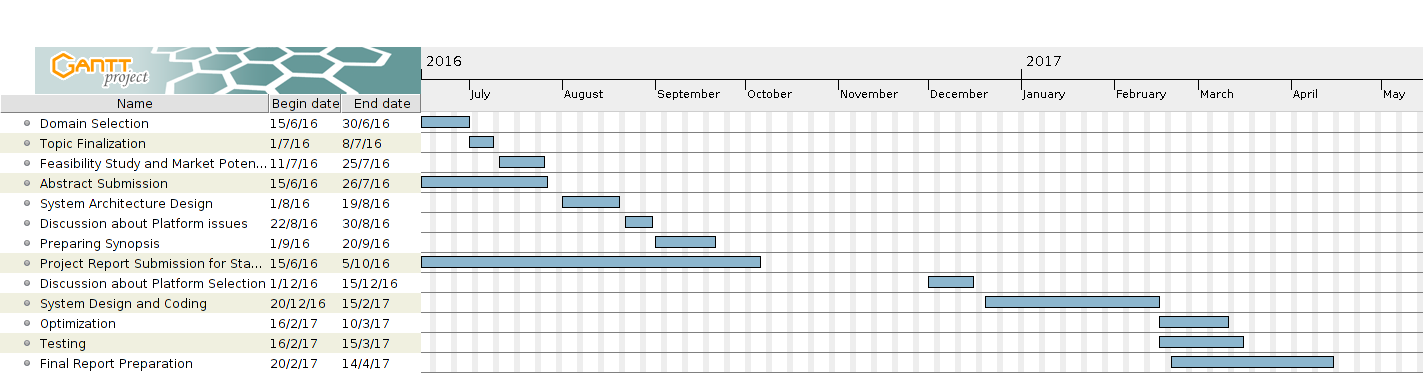
\includegraphics[width=18cm, height=8cm]{gantchart.png}
\caption{Gantt Chart}
\end{figure}

\SkipTocEntry\section{Project Planner - Table}
\begin{table}[h]
\begin{center}
\begin{tabular}{ |p{5cm}|p{3cm}|p{3cm}|p{1.5cm}| } 
 \hline
 \textbf{Name} & \textbf{Start Date} & \textbf{Due Date} & \textbf{Priority} \\ \hline
  Domain Selection & $15^{th}$ June 2016 & $30^{th}$ June 2016 & High \\ \hline
  Topic Finalization & $1^{st}$ July 2016 & $10^{th}$ July 2016 & High \\ \hline
  Feasibility Study and Market Potential Analysis & $11^{th}$ July 2016 & $25^{th}$ July 2016 & High \\ \hline
  Abstract Submission & - & $26^{th}$ July 2016 & Medium \\ \hline
  System Architecture Design & $1^{st}$ Aug 2016 & $20^{th}$ Aug 2016 & High \\ \hline    
  Discussion about Platform issues & $21^{st}$ Aug 2016 & $30^{th}$ Aug 2016 & High \\ \hline
  Preparing Synopsis & $1^{st}$ Sept 2016 & $20^{th}$ sept 2016 & High \\ \hline
  Project Report Submission for Stage I & - & $5^{th}$ Oct 2016 & Medium \\ \hline
  Discussion about Platform Selection & $1^{st}$ Dec. 2016 & $15^{th}$ Dec. 2016 & High \\ \hline
  System Design and Coding & $20^{th}$ Dec. 2016 & $15^{th}$ Feb. 2017 & High \\ \hline
  Testing & $16^{th}$ Feb. 2016 & $15^{th}$ Macrh 2016 & High \\ \hline
  Final Report Preparation & - & $15^{th}$ April 2016 & High \\ \hline
\end{tabular}
\end{center}
\caption{Project Planner}
\end{table}
\newpage

\AddToShipoutPictureBG*{%
\begin{tikzpicture}[overlay,remember picture]
\draw[line width=1.5pt]
    ($ (current page.north west) + (0.7cm,-0.7cm) $)
    rectangle
    ($ (current page.south east) + (-0.7cm,0.7cm) $);
\draw[line width=1.5pt]
    ($ (current page.north west) + (0.9cm,-0.9cm) $)
    rectangle
    ($ (current page.south east) + (-0.9cm,0.9cm) $);
\end{tikzpicture}
}
\SkipTocEntry\chapter{Annexure D}
\thispagestyle{empty}
\newpage
\SkipTocEntry\section{Reviewers Comments of Paper Submitted}
\begin{enumerate}
\item
\textbf{ Paper Title:} Detection of DDoS Attacks in SDN using Support Vector Machine, Entropy Based Discretization and Fuzzy C-Means Clustering.


\item
\textbf{ Name of the Journal: } Springer Journals, Journal of The Institution of Engineers (India): Series B.

\item
\textbf{ Paper accepted/rejected: } Pending.

%\item
%\textbf{ Review comments by reviewer: } None.

%\item
%\textbf{
%Corrective actions if any:
%}
\end{enumerate}
\newpage

\AddToShipoutPictureBG*{%
\begin{tikzpicture}[overlay,remember picture]
\draw[line width=1.5pt]
    ($ (current page.north west) + (0.7cm,-0.7cm) $)
    rectangle
    ($ (current page.south east) + (-0.7cm,0.7cm) $);
\draw[line width=1.5pt]
    ($ (current page.north west) + (0.9cm,-0.9cm) $)
    rectangle
    ($ (current page.south east) + (-0.9cm,0.9cm) $);
\end{tikzpicture}
}
\SkipTocEntry\chapter{Annexure E}
\thispagestyle{empty}
\newpage
\SkipTocEntry\section{Plagiarism Report}
\begin{figure}[h]
\begin{center}
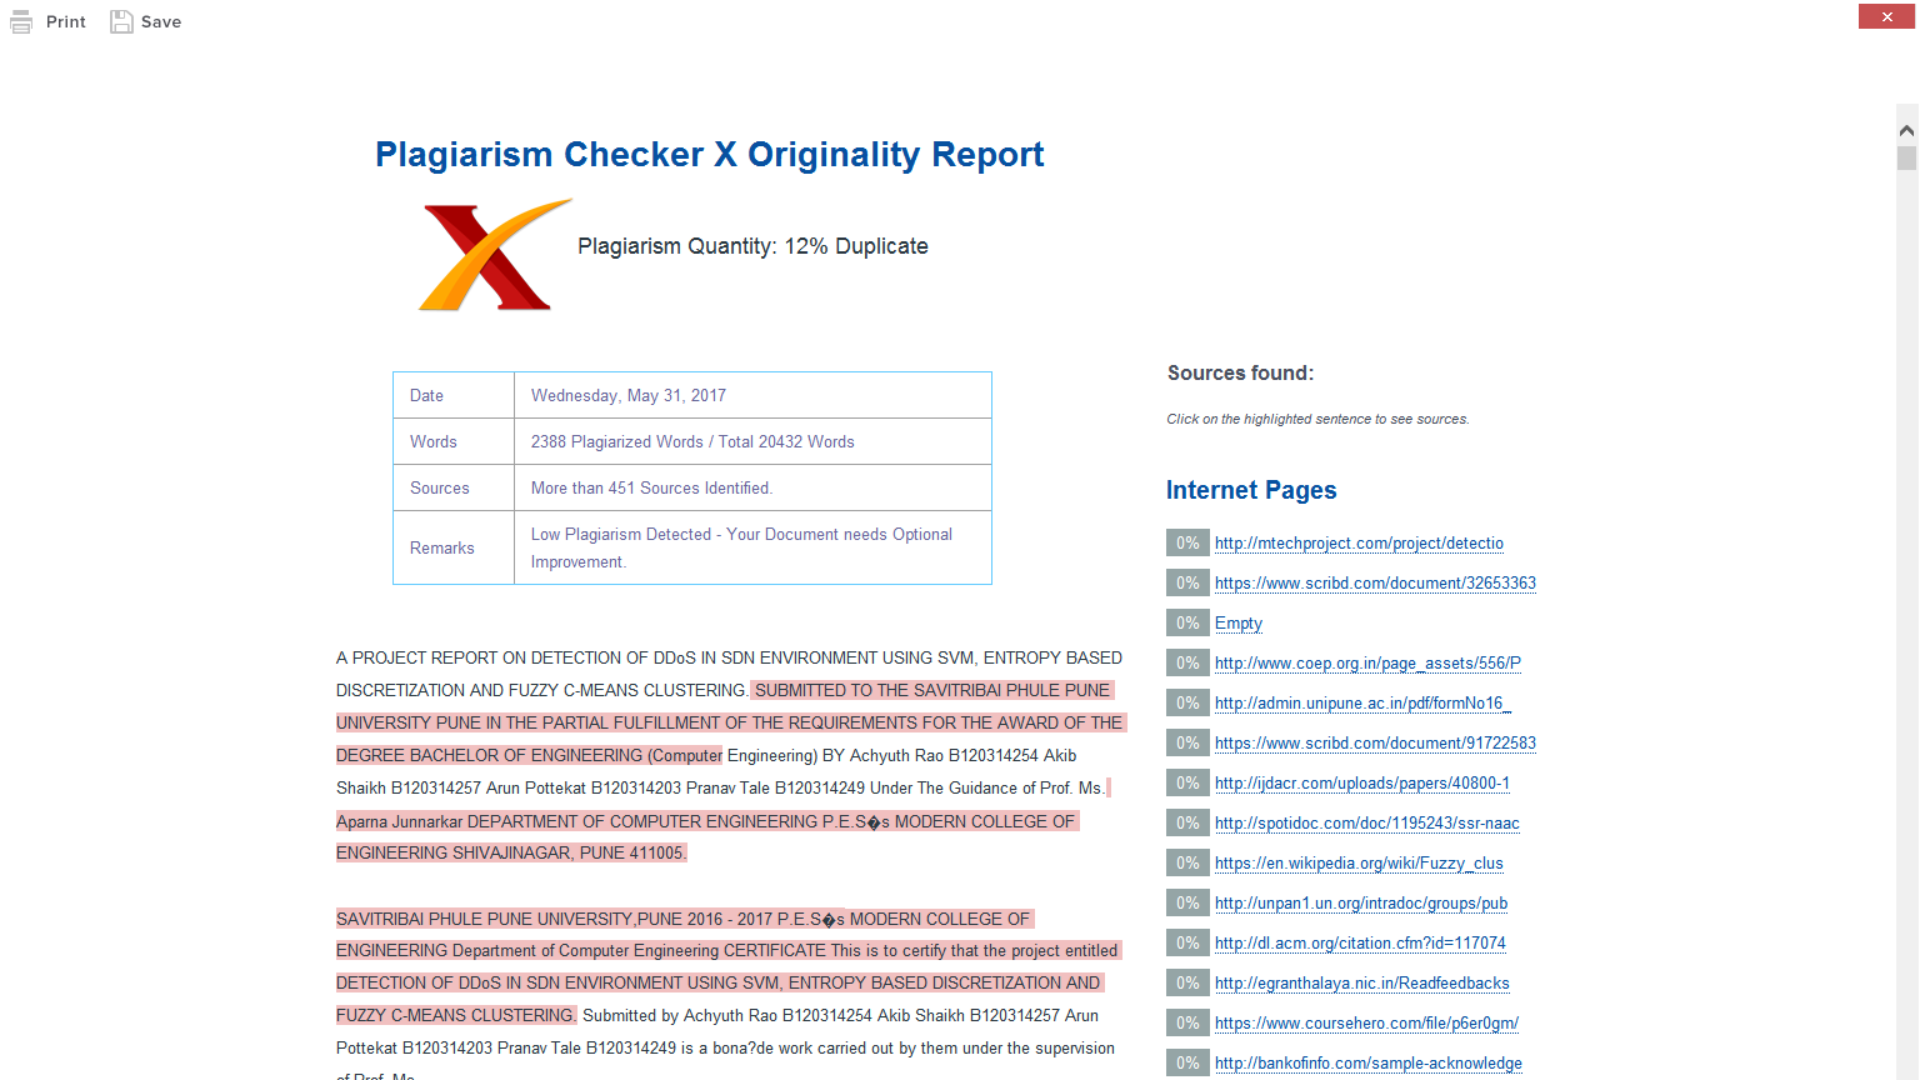
\includegraphics[scale=0.4]{plague1.png}
\caption{Plagiarism Report}
\end{center}
\end{figure}

\begin{figure}[h]
\begin{center}
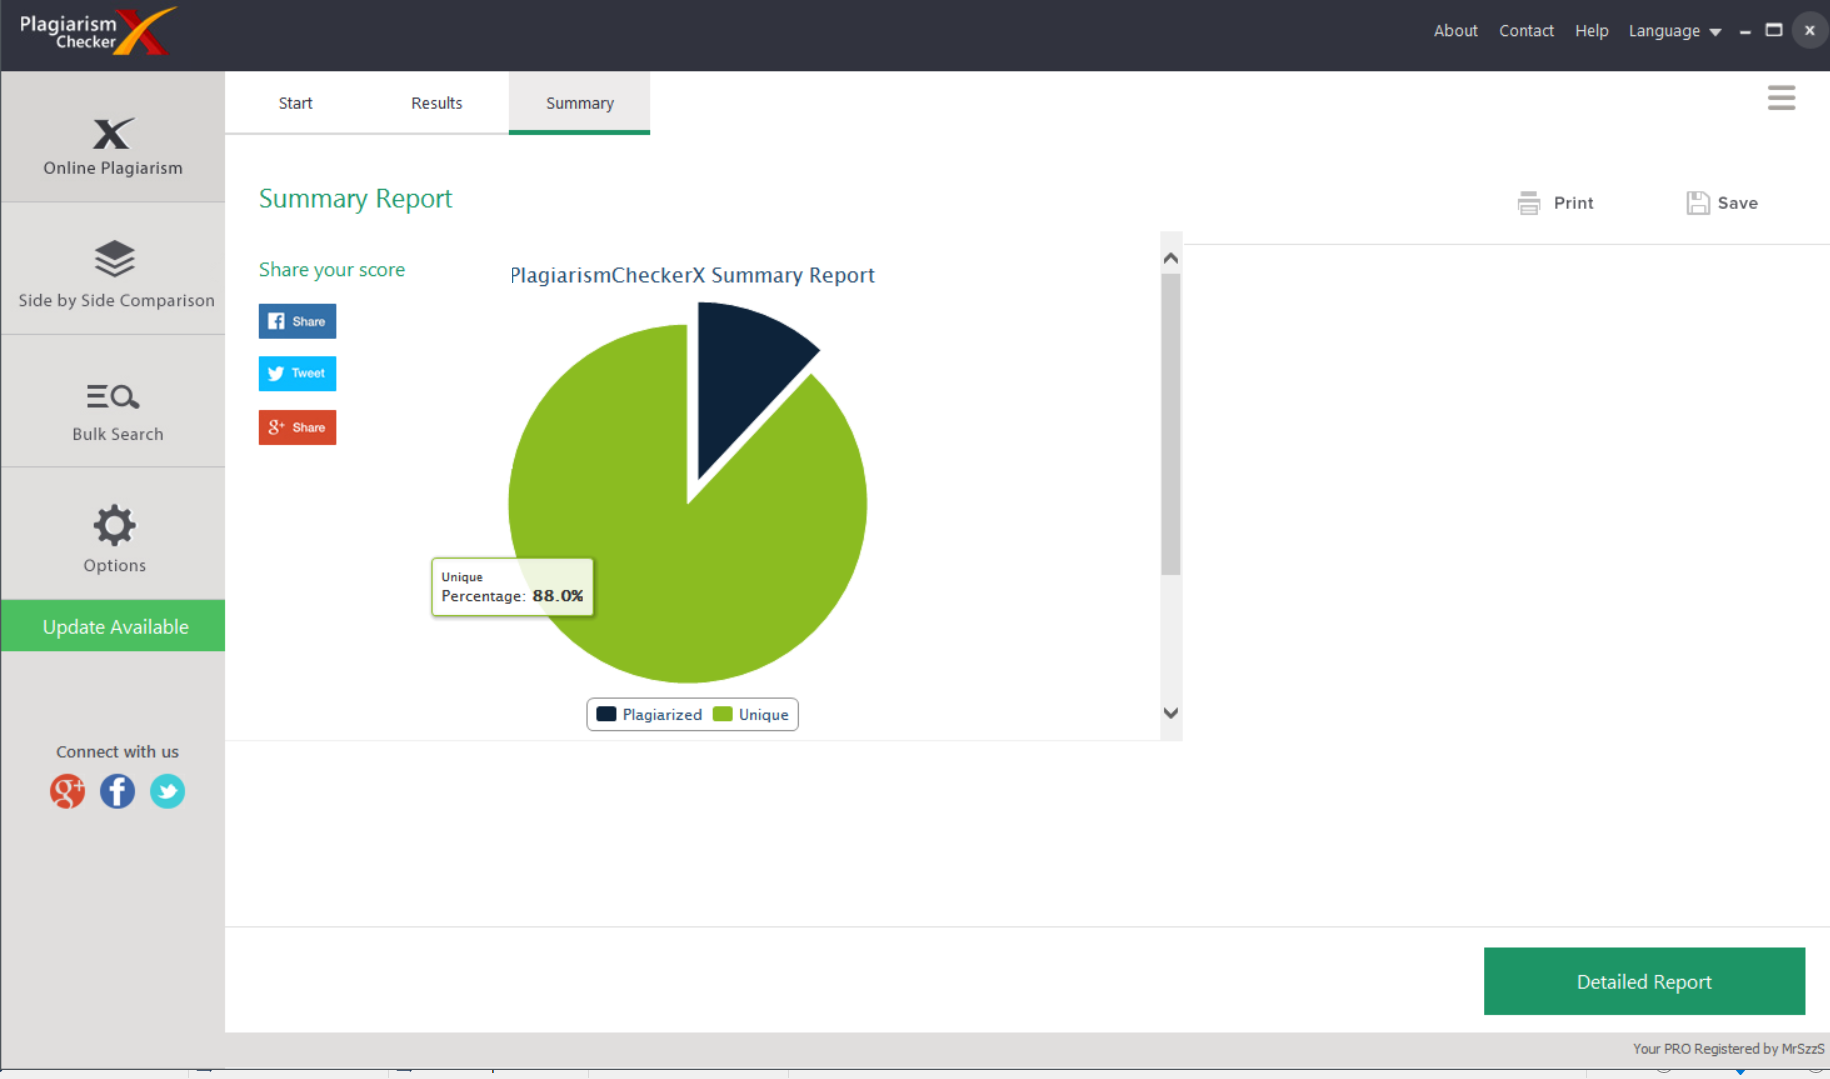
\includegraphics[width=12cm, height=7cm]{plague2.png}
\caption{Plagiarism Report}
\end{center}
\end{figure}
\newpage

\AddToShipoutPictureBG*{%
\begin{tikzpicture}[overlay,remember picture]
\draw[line width=1.5pt]
    ($ (current page.north west) + (0.7cm,-0.7cm) $)
    rectangle
    ($ (current page.south east) + (-0.7cm,0.7cm) $);
\draw[line width=1.5pt]
    ($ (current page.north west) + (0.9cm,-0.9cm) $)
    rectangle
    ($ (current page.south east) + (-0.9cm,0.9cm) $);
\end{tikzpicture}
}
\SkipTocEntry\chapter{Annexure F}
\thispagestyle{empty}
\newpage
\SkipTocEntry\section{Term II Project Laboratory Assignments}
\SkipTocEntry\subsection{Review of Design}
At the end of Term 1 assessment i.e. after completing the design phase of our project the reviews received were :
\begin{enumerate}
\item
To make sure high accuracy will be achieved.
\end{enumerate}

Taking into consideration this review, instead of using libraries for developing the algorithms, the algorithms have been developed right from scratch to mould them into models very specific to the use case of our project i.e. DDoS Detection.
\newline

Along with the feedback report of Term 1 assessment, we had also participated in the annual project competition PICT-Impetus and Concepts 2017, gaining valuable insights and reviews for our project. Industrial personnel belonging to companies like VmWare, Calsoft, Synerzip, ParallelMinds, Veritas, Cybage and many more. Having vast expertise in the domains of our project and were well versed with the latest technologies like SDN, ELK Stack, sFlow. Some of the criticism/feedbacks we received were :
\begin{enumerate}
\item
What kind of DDoS attacks are being detected?

\item
Why mitigation is not being included in the scope of the project?

\item
Change the controller used, from POX to OpenDayLight.

\item
Include adaptive learning module to adapt to the changing network scenarios. 
\end{enumerate}

Some crictics were encouraging and required our attention to be drawn to the issue, one such issue was including the adaptive module to varying network environments. Hence in entropy based discretization we have included the adaptive module which modifies the normal network entropy based on average weighted mean of previous 5 entries of normal entropy.
\newline

Positive feedback was also given stating the innovativeness of the project, inclusion of well known production based tools like ELK Stack, sFlow and replicating a real world environment. 
\newline
These feedbacks highlighted the strong and weak areas in our project which helped us a great deal in tackling the cross questions on the effectiveness of our project.


\SkipTocEntry\subsection{Programming Interfaces}
The programming interfaces for SVM are:-
\begin{enumerate}
\item
\textbf{TShark} - It is network capturing and analysis tool which is used for capturing packet data from a live source, or from a previously captured network stream. It's native capturing file format is pcap format.
\item
\textbf{Numpy} - It is a python library which is used to perform mathematical operations over arrays.
\item
\textbf{Pandas} - It is a python library which is used for statistical data analysis, by performing batch operations rather than line by line operation.
\newpage
\item
\textbf{Flask} - Python micro web development framework.
\newline
Additional components :-
\begin{enumerate}
\item
Flask\_bootstrap

\item
Flask\_wtf

\item
Flask\_blueprint

\item
JQuery-3.0

\item
Flask\_sqlalchemy
\end{enumerate}
\end{enumerate}
\newpage

\AddToShipoutPictureBG*{%
\begin{tikzpicture}[overlay,remember picture]
\draw[line width=1.5pt]
    ($ (current page.north west) + (0.7cm,-0.7cm) $)
    rectangle
    ($ (current page.south east) + (-0.7cm,0.7cm) $);
\draw[line width=1.5pt]
    ($ (current page.north west) + (0.9cm,-0.9cm) $)
    rectangle
    ($ (current page.south east) + (-0.9cm,0.9cm) $);
\end{tikzpicture}
}
\SkipTocEntry\chapter{Annexure G}
\thispagestyle{empty}
\newpage
\SkipTocEntry\section{Information of Project Group Members}
\begin{flushright}
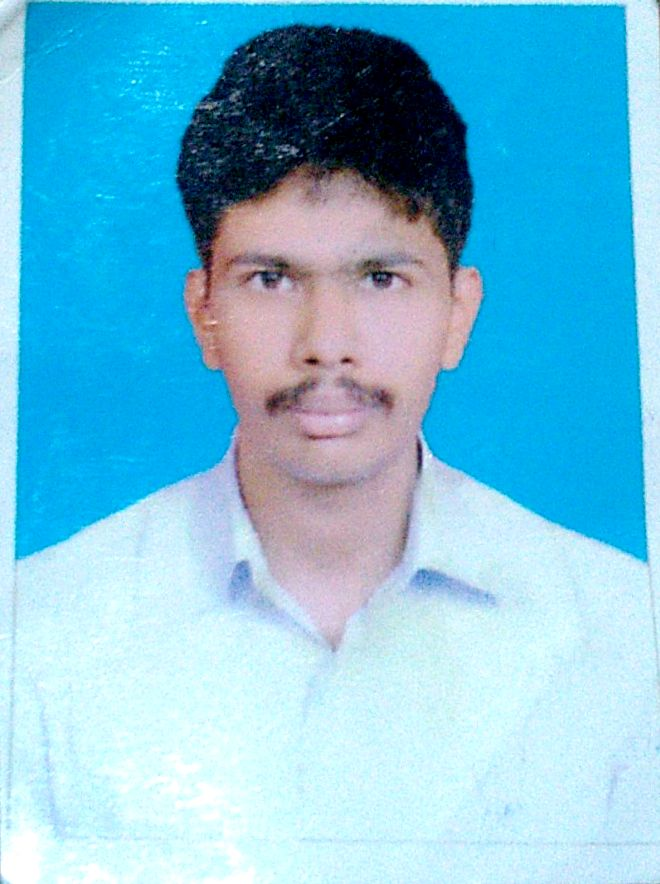
\includegraphics[width=60pt]{Achyuth.jpg}
\end{flushright}

\begin{enumerate}
\item Name : S. Achyuth Rao
\item Date of Birth : $19^{th}$ November, 1995
\item Gender : Male
\item Permanent Address : S-4, Mangalam apts., Tingre Nagar, Pune.
\item E-Mail : aachyutha2@gmail.com
\item Mobile/Contact No. : 07798845233
\item Placement Details : None
\item Paper Published : None

\end{enumerate}

\newpage
\begin{flushright}

\includegraphics[width=60pt]{akib.jpg}
\end{flushright}

\begin{enumerate}
\item Name : Akib A. Shaikh
\item Date of Birth : $26^{th}$ April, 1996
\item Gender : Male
\item Permanent Address : 519, Centre Street, Camp, Pune.
\item E-Mail : akibshaikh117@gmail.com
\item Mobile/Contact No. : 09763851944
\item Placement Details : TCS Ltd.
\item Paper Published : None

\end{enumerate}
\newpage
\begin{flushright}
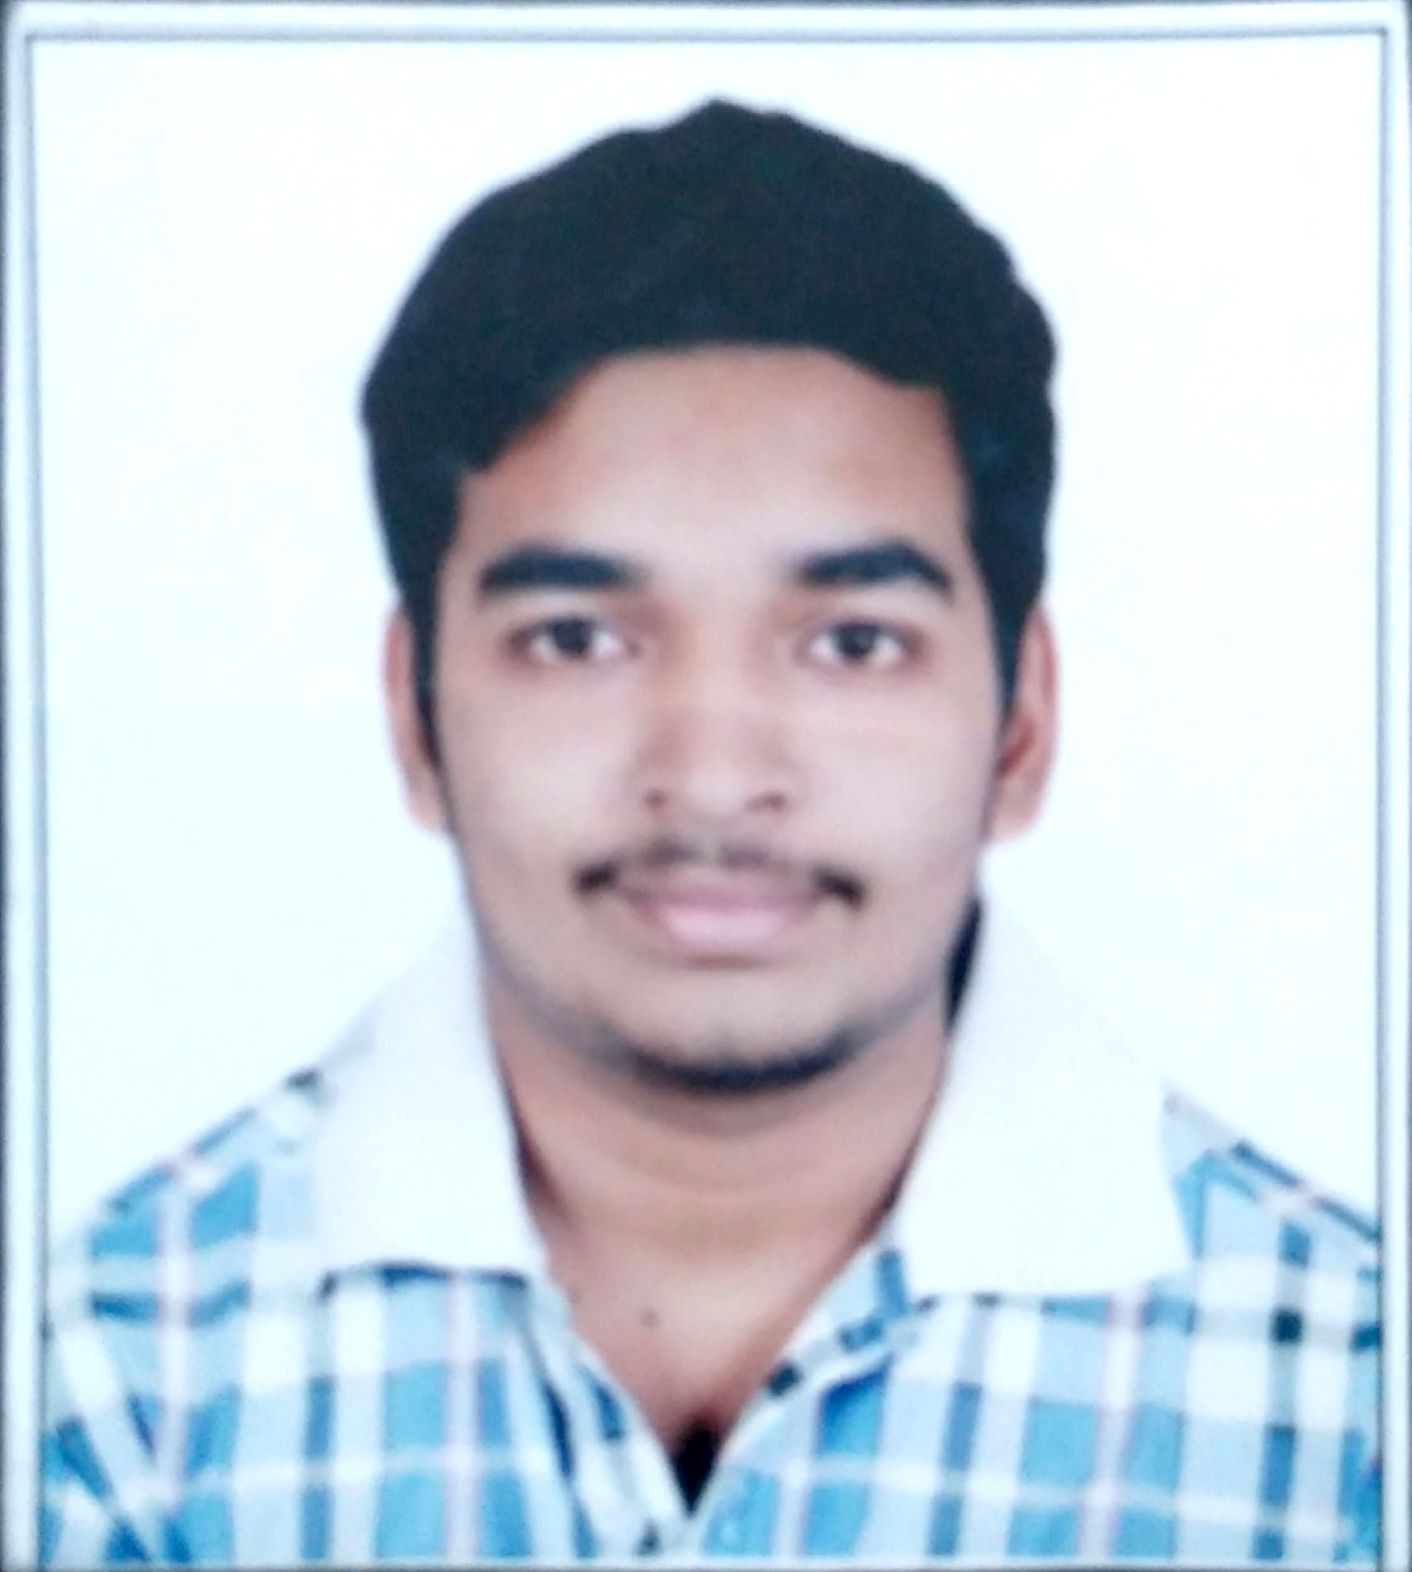
\includegraphics[width=60pt]{arun.jpg}
\end{flushright}

\begin{enumerate}
\item Name : Arun P. Pottekat
\item Date of Birth : $22^{nd}$ June, 1995
\item Gender : Male
\item Permanent Address : Citadel E/18, Ghorpadi, Pune.
\item E-Mail : apottekat@gmail.com		
\item Mobile/Contact No. : 09561120935
\item Placement Details : None
\item Paper Published : None

\end{enumerate}

\newpage
\begin{flushright}
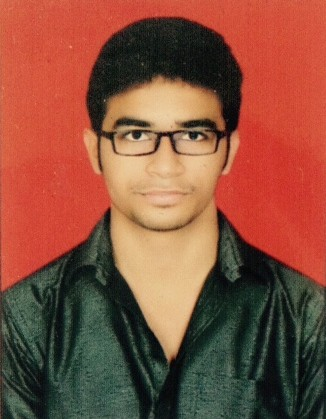
\includegraphics[width=60pt]{pranav.JPG}
\end{flushright}

\begin{enumerate}
\item Name : Pranav B. Tale
\item Date of Birth : $16^{th}$ June, 1995
\item Gender : Male
\item Permanent Address : 107-B, Rathi Nagar, Amravati, Maharashtra.
\item E-Mail : pranav.tale@gmail.com
\item Mobile/Contact No. : 09730692749
\item Placement Details : TCS Ltd.
\item Paper Published : None

\end{enumerate}
\end{document}\documentclass[12pt,a4paper,final]{report}
\usepackage[english]{babel}
\usepackage[fleqn]{amsmath}
\usepackage{amsfonts}
\usepackage{amssymb}
\usepackage{mathptmx}
\usepackage{fancyhdr}
\usepackage{graphicx}
\usepackage{array}
\usepackage{wrapfig}
\usepackage{algorithm}
\usepackage{algpseudocode}

\usepackage[%
    a4paper,
%   includeheadfoot,
    head=0.762cm,  % distance from bottom of header to block of text aka \headsep e.g. \baselineskip
    foot=0.762cm,  % distance from top of footer to block of text aka \footskip
    headheight=12pt,     % height for the header block (no equivalent for footer)
%   heightrounded,       % ensure an integer number of lines
    marginparwidth=2cm,  % right marginal note width
    marginparsep=2mm,    % distance from text block to marginal note box
%   height=\textheight,  % height of the text block
%   width=\textwidth,    % width of the text block
    top=1.7cm,           % distance of the text block from the top of the page
    bottom=1.4cm,
    left=1.9cm,
    right=1.9cm,
%    showframe,           % show the main blocks
%    verbose,             % show the values of the parameters in the log file
]{geometry}

\pagestyle{fancy}
\fancyhf{}
\rhead{\bfseries {\nouppercase{\leftmark}}}
\lhead{\bfseries DDoS Detection in Software Defined Network}
\cfoot{PESMCOE,Department of Computer Engineering 2016-17}
\rfoot{\thepage}

\usepackage[table]{xcolor}
\newcolumntype{P}[1]{>{\centering\arraybackslash}p{#1}}
\newcolumntype{M}[1]{>{\centering\arraybackslash}m{#1}}
 
\renewcommand{\footrulewidth}{0.4pt}

\title{Detection of DDoS in SDN environment using SVM and Entropy based discretization.}
\graphicspath{ {Images/} }

\usepackage{tikz}
\usetikzlibrary{calc}
\usepackage{eso-pic}

\usepackage{titlesec}
\titleformat{\section}[block]
  {\fontsize{16}{18}\bfseries}
  {\thesection}
  {1em}
  {}
\titleformat{\subsection}[block]
  {\fontsize{14}{15}\bfseries}
  {\thesubsection}
  {1em}
  {}

\usepackage{blindtext}
\usepackage{tocloft}
\renewcommand{\cfttoctitlefont}{\hspace*{\fill}\Huge\bfseries}
\renewcommand{\cftaftertoctitle}{\hspace*{\fill}}
\renewcommand{\cftlottitlefont}{\hspace*{\fill}\Huge\bfseries}
\renewcommand{\cftafterlottitle}{\hspace*{\fill}}
\renewcommand{\cftloftitlefont}{\hspace*{\fill}\Huge\bfseries}
\renewcommand{\cftafterloftitle}{\hspace*{\fill}}

\newcommand{\abbrlabel}[1]{\makebox[6cm][l]{\textbf{#1}\ \dotfill}}
\newenvironment{abbreviations}{\begin{list}{}{\renewcommand{\makelabel}{\abbrlabel}}}{\end{list}}

\DeclareRobustCommand{\gobblefive}[5]{}
\newcommand*{\SkipTocEntry}{\addtocontents{toc}{\gobblefive}}

\usepackage{hyperref}
\hypersetup{
    colorlinks=true,
    linkcolor=black,
    citecolor=black,
}

\begin{document}
\begin{center}
\thispagestyle{empty}
\vspace*{1cm}
A PROJECT REPORT ON
\vspace*{0.75cm}

\Large
\textbf{
DETECTION OF DDoS IN SDN ENVIRONMENT USING SVM, ENTROPY  BASED DISCRETIZATION AND FUZZY C-MEANS CLUSTERING.
}
\vspace*{0.75cm}

\normalsize
SUBMITTED TO THE SAVITRIBAI PHULE PUNE UNIVERSITY PUNE IN THE PARTIAL FULFILLMENT OF THE REQUIREMENTS FOR THE AWARD OF THE DEGREE
\vspace*{0.5cm}

\large
\textbf{
BACHELOR OF ENGINEERING\\
(Computer Engineering)\\
\vspace*{0.3cm}
BY\\
}
\vspace*{0.3cm}
\normalsize
Achyuth Rao \hspace*{2.2cm} B120314254 \\
Akib Shaikh \hspace*{2.4cm} B120314257 \\
Arun Pottekat \hspace*{2.2cm} B120314203 \\
Pranav Tale \hspace*{2.5cm} B120314249 \\
\vspace*{0.4cm}

\large
\textbf{
Under The Guidance of \\
}
\normalsize
\vspace*{0.2cm}
Prof. Ms. Aparna Junnarkar

\normalsize
\begin{figure}[h]
\begin{center}

\includegraphics[width=3cm, height=4cm]{collegelogo.png}
\end{center}
\end{figure}

\textbf{
\large
\vspace*{0.2cm}
DEPARTMENT OF COMPUTER ENGINEERING \\
P.E.S's MODERN COLLEGE OF ENGINEERING \\
}
\normalsize
SHIVAJINAGAR, PUNE 411005. \\
\textbf{
\large
\linebreak
\vspace*{0.2cm}
SAVITRIBAI PHULE PUNE UNIVERSITY,PUNE \\
2016 - 2017 
}
\end{center}
\newpage

\thispagestyle{empty}
\vspace*{1.3cm}

\includegraphics[width=2cm, height=2.5cm]{collegelogo.png}
\vspace*{-2.5cm}
\begin{center}
\normalsize
\textbf{
P.E.S's MODERN COLLEGE OF ENGINEERING \\
\vspace*{0.25cm}
Department of Computer Engineering \\
}
\vspace{3cm}

\Large
\textbf{CERTIFICATE}
\end{center}
\normalsize
\vspace{0.5cm}
\begin{center}
This is to certify that the project entitled \\
\large
\vspace*{0.3cm}
\textbf{
DETECTION OF DDoS IN SDN ENVIRONMENT USING SVM, ENTROPY  BASED DISCRETIZATION AND FUZZY C-MEANS CLUSTERING. \\
}
\vspace*{0.5cm}
\normalsize
Submitted by \\
Achyuth Rao \hspace*{2.2cm} B120314254 \\
Akib Shaikh \hspace*{2.4cm} B120314257 \\
Arun Pottekat \hspace*{2.2cm} B120314203 \\
Pranav Tale \hspace*{2.5cm} B120314249 \\
\end{center}
\vspace{1cm}
is a bonafide work carried out by them under the supervision of Prof. Ms. Aparna Junnarkar and it is approved for the partial fulfillment of the requirement of Savtribai Phule Pune university, Pune for the award of the degree of Bachelor of Engineering (Computer Engineering). \vspace{2.5cm}\\
\hspace*{0.8cm}
Prof. Ms. Aparna Junnarkar
\hspace{6cm}
Prof. Dr. Mrs. S. A. Itkar \\
\hspace*{2.5cm}
Guide
\hspace{10cm}
Head \\
\hspace*{1cm}
Dept. of Computer Engg.
\hspace{6.4cm}
Dept. of Computer Engg. \\
\begin{minipage}{\textwidth}
\vspace{2cm}
\hspace*{0.7cm}
Signature of Internal Examiner
\hspace{5.5cm}
Signature of External Examiner
\end{minipage}

\newpage
\thispagestyle{empty}
\large
\begin{center}
\vspace*{2cm}
PROJECT APPROVAL SHEET \\
\normalsize
A Project Report Titled as \\ 

\vspace*{2cm}

\Large
\textbf{
DETECTION OF DDoS IN SDN ENVIRONMENT USING SVM,
ENTROPY BASED DISCRETIZATION AND FUZZY C-MEANS
CLUSTERING.
}

\normalsize
\vspace*{3cm}
Is verified for its originality in documentation, problem statement, proposed work and implementation successfully completed by \\ 

\vspace{0.5cm}
Achyuth Rao \hspace*{2.2cm} B120314254 \\
Akib Shaikh \hspace*{2.4cm} B120314257 \\
Arun Pottekat \hspace*{2.2cm} B120314203 \\
Pranav Tale \hspace*{2.5cm} B120314249 \\

\vspace{0.5cm}
at \\
\vspace{0.5cm}
DEPARTMENT OF COMPUTER ENGINEERING \\
\vspace{0.5cm}
PES MODERN COLLEGE OF ENGINEERING \\
\vspace{0.5cm}
SAVITRIBAI PHULE PUNE UNIVERSITY,PUNE \\
\vspace{0.5cm}
ACADEMIC YEAR 2016-2017 \\

\vspace{3cm}
\hspace*{0.8cm}
Prof. Ms. Aparna Junnarkar
\hspace{6cm}
Prof. Dr. Mrs. S. A. Itkar \\
\hspace*{0.8cm}
Guide
\hspace{9.6cm}
H.O.D. \\
\hspace*{1cm}
Dept. of Computer Engg.
\hspace{6.4cm}
Dept. of Computer Engg. \\
\end{center}

\thispagestyle{empty}
\Large
\begin{center}
\chapter*{\centering Acknowledgement}
\pagenumbering{gobble}
\end{center}
\normalsize
It gives us pleasure in presenting the preliminary project report on \textbf{`Detection of Distributed Denial of service attack in Software Defined Network using Support Vector Machine, Entropy Based Discretization and Fuzzy C Means Clustering'}.\\

Firstly, we would like to express our indebtedness appreciation to our internal guide \textbf{Ms. Aparna A. Junnarkar}. Her constant guidance and advice played very important role in making the execution of the report. She always gave us her suggestions, that were crucial in making this report as flawless as possible.\\

We would like to express our gratitude towards \textbf{Prof. Dr. Mrs. S. A. Itkar}  Head of Computer Engineering Department, PES Modern College of Engineering for her kind co-operation and encouragement which helped us during the completion of this report.\\

Also, we would like to thank \textbf{Mr. Kunal Khadke, Ms. Yogita Narwadkar, Mr. B. D. Phulpagare, Ms. Pallavi Baviskar, Ms. Deipali V. Gore, Ms. Renuka Kajale} and all \textbf{Technical assistants} for providing time to time guidance and various resources such as laboratory with all needed software platforms and continuous Internet connection for our Project.\\

In the end special thanks to all our classmates for helping us out during the entire documentation process.

\vspace{3cm}
\begin{flushright}
Achyuth Rao\\
Akib Shaikh\\
Arun Pottekat\\
Pranav Tale\\
(B.E. Computer Engineering)
\end{flushright}
\newpage

\pagestyle{plain} 
\cleardoublepage
\pagenumbering{gobble}
\tableofcontents
\newpage

\pagenumbering{roman}
\Large
\chapter*{\centering Abstract}
\addcontentsline{toc}{chapter}{Abstract}
\normalsize
\noindent
The current networking paradigm involves switches, routers and gateways where these networkingdevices constitute both logical thinking as well as routing of packets. Traditionally the network ad-ministrator is responsible for configuring and managing these devices manually and at all times, which makes it a tedious task.

With the onset of the Software Defined Network, this task of manually managing the devices re-duces to some extent, as it seperates the control plane from the data plane i.e. Forwarding of packets is done in the data plane and intelligence of the entire network resides in the control plane.

Data plane constitutes the network devices which comprise switches known as ”dumb terminals” and the control plane constitutes a central controller which keeps track of all switches in the network.

Due to the centralized nature of SDN i.e. the controller at the center of SDN taking the logicaldecisions, there arises a threat of malicious users launching cyber attacks on this central component thereby, dislodging the entire network. Some attacks include Application level attacks, Brute Force attack, man in the middle attacks, DDoS attack etc.

Distributed Denial of Service attack involves a single malicious user controlling different users known as bots to launch an attack against a single entity in the network without even the victim being aware of the attack. DDoS attacks result in direct financial losses along with damage to company reputation and loss of the customer’s trust.

As a part of solution to this problem, three algorithms can be used for the detection of DDoS attack i.e. Support Vector Machine, a machine learning algorithm and Entropy based Discretization and Fuzzy C-Means Clustering, two Data Mining algorithms.

Support Vector Machine takes the rate of incoming packets as the input and classifies them as normal traffic or attack traffic. Whereas Entropy based Discretization monitors the entropy of the network i.e. measure of randomness and if it falls below a threshold value then it is classified as attack traffic and Fuzzy C-Means Clustering clusters the incoming packets into normal or attack classes.

Once the attack is detected by either of the applications, an entry will be made in the log files constantly monitored by network monitoring tools and thus report the incident back to the network adminstrative team.

The network adminstrator would be provided a monitoring application which would display the details of the attack detected such as the source IP and victim IP etc.

As a part of the project, comparison studies will also be done related to both algorithms displaying the rate at which attacks are detected along with their accuracies.
\newpage

\listoffigures
\addcontentsline{toc}{chapter}{List of Figures}
\newpage
\listoftables
\addcontentsline{toc}{chapter}{List of Tables}
\newpage

\chapter*{\centering List of Abbreviations}
\begin{abbreviations}
\item[SDN] Software Defined Network
\item[SVM] Support Vector Machine
\item[DDoS] Distributed Denial of Service
\item[ONOS] Open Network Operating Switch
\item[OVSDB] Open vSwitch Database
\item[EBD] Entropy based Discretization
\item[NP] Non Polynomial Time
\item[P] Polynomial Time
\item[FCM] Fuzzy C Means 
\item[HTTP] Hyper Text Transfer Protocol
\item[UDP] Uniform Datagram Protocol
\item[TCP] Transmission Control Protocol
\item[k-NN] K Nearest Neighbour
\item[ICMP] Internet Control Message Protocol
\item[FTP] File Transfer Protocol
\item[QP] Quadratic problem
\end{abbreviations}

\addcontentsline{toc}{chapter}{List of Abbreviations}
\newpage
\pagestyle{fancy}
 
\newcommand{\hsp}{\hspace{0pt}}
\titleformat{\chapter}[hang]
{\flushright\fontseries{b}\fontsize{80}{100}\selectfont}{\fontseries{b}\fontsize{72}{84}\selectfont\textcolor{black}\thechapter\hsp}{0pt}
{.\\ \Huge\bfseries}
[]\titlespacing*{\chapter}{0pt}{540pt}{20pt}	

\pagenumbering{gobble}
\pagenumbering{arabic}

\AddToShipoutPictureBG*{%
\begin{tikzpicture}[overlay,remember picture]
\draw[line width=1.5pt]
    ($ (current page.north west) + (0.7cm,-0.7cm) $)
    rectangle
    ($ (current page.south east) + (-0.7cm,0.7cm) $);
\draw[line width=1.5pt]
    ($ (current page.north west) + (0.9cm,-0.9cm) $)
    rectangle
    ($ (current page.south east) + (-0.9cm,0.9cm) $);
\end{tikzpicture}
}
\chapter{Synopsis}
\thispagestyle{empty}
\newpage
\section{Project Title}
Detection of DDoS in SDN environment using SVM, Entropy based Discretization and Fuzzy C-mean Clustering.

\section{Project Option}
Internal Project

\section{Internal Guide}
Prof. Mrs. Aparna Junnarkar

\section{Technical Keywords}
\begin{enumerate}
\item C. Computer Systems Organization 
\begin{enumerate}
\item C.2 COMPUTER-COMMUNICATION NETWORKS 
\begin{enumerate}
\item C.2.0 General  
\begin{enumerate}
\item  Security and protection
\end{enumerate} 
\item C.2.1 Network Architecture and Design
\begin{enumerate}
\item  Centralized networks
\end{enumerate} 
\end{enumerate} 
\end{enumerate}
	
\item H. Information Systems  
\begin{enumerate}
\item H.2 DATABASE MANAGEMENT
\begin{enumerate}		
\item H.2.8 Database Applications   
\begin{enumerate}
\item  Data mining
\end{enumerate} 	 		
\end{enumerate} 
\end{enumerate}	

\begin{enumerate}
\item H.3 INFORMATION STORAGE AND RETRIEVAL 
\begin{enumerate}		
\item H.3.3 Information Search and Retrieval  
\begin{enumerate}
\item  Clustering
\item Information filtering
\end{enumerate} 
\end{enumerate} 
\end{enumerate}
	
\item I. Computing Methodologies  
\begin{enumerate}
\item I.5 PATTERN RECOGNITION 
\begin{enumerate}		
\item I.5.3 Clustering   
\begin{enumerate}
\item Algorithms
\item Similarity measures 
\end{enumerate} 
\end{enumerate} 
\end{enumerate}		
\end{enumerate}

\section{Problem Statement}
To provide a solution for the detection of DDoS attack in SDN environment
using SVM, Entropy based Discretization, Fuzzy C-mean Clustering and monitoring OpenFlow statistics.

\section{Abstract}
The current networking paradigm involves switches, routers and gateways where these networkingdevices constitute both logical thinking as well as routing of packets. Traditionally the network ad-ministrator is responsible for configuring and managing these devices manually and at all times, which makes it a tedious task.

With the onset of the Software Defined Network, this task of manually managing the devices re-duces to some extent, as it seperates the control plane from the data plane i.e. Forwarding of packets is done in the data plane and intelligence of the entire network resides in the control plane.

Data plane constitutes the network devices which comprise switches known as ”dumb terminals” and the control plane constitutes a central controller which keeps track of all switches in the network.

Due to the centralized nature of SDN i.e. the controller at the center of SDN taking the logicaldecisions, there arises a threat of malicious users launching cyber attacks on this central component thereby, dislodging the entire network. Some attacks include Application level attacks, Brute Force attack, man in the middle attacks, DDoS attack etc.

Distributed Denial of Service attack involves a single malicious user controlling different users known as bots to launch an attack against a single entity in the network without even the victim being aware of the attack. DDoS attacks result in direct financial losses along with damage to company reputation and loss of the customer’s trust.

As a part of solution to this problem, three algorithms can be used for the detection of DDoS attack i.e. Support Vector Machine, a machine learning algorithm and Entropy based Discretization and Fuzzy C-Means Clustering, two Data Mining algorithms.

Support Vector Machine takes the rate of incoming packets as the input and classifies them as normal traffic or attack traffic. Whereas Entropy based Discretization monitors the entropy of the network i.e. measure of randomness and if it falls below a threshold value then it is classified as attack traffic and Fuzzy C-Means Clustering clusters the incoming packets into normal or attack classes.

Once the attack is detected by either of the applications, an entry will be made in the log files constantly monitored by network monitoring tools and thus report the incident back to the network adminstrative team.

The network adminstrator would be provided a monitoring application which would display the details of the attack detected such as the source IP and victim IP etc.

As a part of the project, comparison studies will also be done related to both algorithms displaying the rate at which attacks are detected along with their accuracies.


\section{Goals and Objective}
\begin{enumerate}
\item
Detect DDoS and generate an alert for the network administrative team.

\item
Compare three solutions by integrating the concepts of Software Defined Networking with Support Vector Machine, Entropy based Discretization and Fuzzy C-Means.

\item
Monitoring OpenFlow Statistics using sFlow and log monitoring using Elasticsearch, Logstach and Kibana (ELK Stack).
\end{enumerate}

\newpage
\section{Relevant mathematics associated with the Project}
\begin{itemize}
\item Input: Network Statistics.
\item Output: DDoS detected or not detected.
\item Data Structure: Python dictionary
\item Function Relation: DDoS alert will be generated if one or more functions detects the attack traffic.
\item As, our DDoS detection mechanism will work on the switches distributed throughout the network. Hence, we are using distributed processing.
\item Mathematical formulas: 
\begin{flushleft}
\begin{itemize}
\item SVM:
\linebreak
\begin{equation}
y = \overline{\omega} * x + b
\end{equation}
\linebreak
This Formula is used for calculating the classification value for a given data point.
		 
\item Entropy based Discretization:
\linebreak
\begin{equation}
\varepsilon = \sum_{i=0}^{n} - P_{i} log P_{i}
\end{equation}

This Formula is used to calculate the Entropy value of Network.
		
\item Fuzzy C-mean Clustering:
\linebreak
\begin{equation}
C_{i} = \frac{\sum_{j=1}^{n}u_{ij}^{m}X_{ij}}{\sum_{n}^{j=1}u_{ij}^{m}}
\end{equation}

Formula to calculate centroid values. \\
\begin{equation}
u_{ij} = \frac{\frac{-2}{d_{ij}^{m-1}}}{\sum_{i=1}^{c}{{d_{ij}^{m-1}}}}
\end{equation}

Formula to calculate membership values.
\end{itemize}
\end{flushleft}	
	
\item Success Conditions: 
\begin{itemize}
\item If DDoS attack is launched then an alert is generated.
\item If DDoS attack is not launched then an alert is not generated.
\end{itemize}
	
\item Failure Conditions:
\begin{itemize}
\item Network not established.
\item Controller is not functioning.
\item Packet capturing unsuccessful.
\end{itemize}		

\end{itemize}

\newpage
\section{Names of Conferences / Journals where papers can be published}
\begin{itemize}
\item IEEE / Journal of Security and Privacy.
\item IEEE / Conference on Computer Network.
\item ACM / ACM Transactions on Network Security.
\item ELSEVIER / Journal of Network Security.
\item Springer / Journal of Communication Network.
\end{itemize}
\newpage

\AddToShipoutPictureBG*{%
\begin{tikzpicture}[overlay,remember picture]
\draw[line width=1.5pt]
    ($ (current page.north west) + (0.7cm,-0.7cm) $)
    rectangle
    ($ (current page.south east) + (-0.7cm,0.7cm) $);
\draw[line width=1.5pt]
    ($ (current page.north west) + (0.9cm,-0.9cm) $)
    rectangle
    ($ (current page.south east) + (-0.9cm,0.9cm) $);
\end{tikzpicture}
}
\chapter{Technical Keywords}
\thispagestyle{empty}
\newpage
\section{Area of Project}
\begin{itemize}
\item Networking
\item Machine Learning
\item Data Mining
\end{itemize}

\section{Technical Keywords}
\begin{enumerate}
\item C. Computer Systems Organization 
\begin{enumerate}
\item C.2 COMPUTER-COMMUNICATION NETWORKS 
\begin{enumerate}
\item C.2.0 General  
\begin{enumerate}
\item  Security and protection
\end{enumerate} 
\item C.2.1 Network Architecture and Design
\begin{enumerate}
\item  Centralized networks
\end{enumerate} 
\end{enumerate} 
\end{enumerate}
	
\item H. Information Systems  
\begin{enumerate}
\item H.2 DATABASE MANAGEMENT
\begin{enumerate}		
\item H.2.8 Database Applications   
\begin{enumerate}
\item  Data mining
\end{enumerate} 
	 		
\end{enumerate} 
\end{enumerate}	
\begin{enumerate}
\item H.3 INFORMATION STORAGE AND RETRIEVAL 
\begin{enumerate}		
\item H.3.3 Information Search and Retrieval  
\begin{enumerate}
\item  Clustering
\item Information filtering
\end{enumerate} 
	 		
\end{enumerate} 
\end{enumerate}
	
\item I. Computing Methodologies  
\begin{enumerate}
\item I.5 PATTERN RECOGNITION 
\begin{enumerate}		
\item I.5.3 Clustering   
\begin{enumerate}
\item Algorithms
\item Similarity measures 
\end{enumerate} 
	 		
\end{enumerate} 
\end{enumerate}	
\end{enumerate}
\newpage

\AddToShipoutPictureBG*{%
\begin{tikzpicture}[overlay,remember picture]
\draw[line width=1.5pt]
    ($ (current page.north west) + (0.7cm,-0.7cm) $)
    rectangle
    ($ (current page.south east) + (-0.7cm,0.7cm) $);
\draw[line width=1.5pt]
    ($ (current page.north west) + (0.9cm,-0.9cm) $)
    rectangle
    ($ (current page.south east) + (-0.9cm,0.9cm) $);
\end{tikzpicture}
}
\chapter{Introduction}
\thispagestyle{empty}
\newpage
\section{Purpose}
The SDN architecture involves the separation of the control plane and the data plane. However this architecture brings to light many security issues. SDN market is expected to reach 12.5 billion dollars by the year 2020. As the number of SDN deployments increase it becomes a necessity to solve these security issues and threats. A successful Distributed Denial of Service (DDoS) attack can make the resources unavailable and cripple the entire network. 

By bringing down the complete operation of the network and exhausting the resources a single DDoS attack can cause a huge loss to an organization.  Therefore effective solutions are required to detect the DDoS attack as early as possible with high accuracy. For the prevention of any attack it's early detection is very necessary. On detecting the DDoS attack effective measures can be taken to prevent it so as to protect the network from the malicious activity initiated by the attackers. This project aims to solve the security issues so as to accelerate the adoption of SDN. 

\section{Project Idea}
Software Defined Networking(SDN) is a promising approach that enables superior network control by providing the ability to change, manage and control, the behaviour of the network and the network devices in a dynamic manner. The separation of control plane (responsible for taking networking decisions) from the data plane (responsible for forwarding the packets) introduces programmability into the network. 

This project combines the concepts of next-generation networking along with machine learning and data mining approaches in order to solve the security issues in SDN. Our aim is to detect the DDoS attack using either Support Vector Machine (SVM) Classifier, Entropy Based Discretization or Fuzzy C Means Clustering and generate an alert so that later it can be effectively mitigated. The acceptance of a solution in an industry depends on its successful functioning in a real world scenario. We propose and compare three solutions for detection of DDoS attack. Support Vector Machine Classifier is a solution based on Machine Learning whereas Entropy-Based Discretization and Fuzzy C Means Clustering are based on data mining. The final solution will be such that it can actually be used in the SDN deployed environments.

\section{Literature Survey}
\subsection{Deciding the Project Topic}
Initially, deciding the project title was a big task in itself. In recent years there has been a huge increase in the use of open source software and technologies, and contributing some work to the open source community would be a great achievement. Everything is future is going to be virtualized as it has already been achieved for computing and storage. In these recent years it was time that traditional networking which was into operation since past 20 years gets changed with the help of research and innovation. 

Software Defined Networking[1][2][3] is a new and promising approach that introduces programmability into the network and is changing the way networking is done since years. But the adoption of SDN by various enterprises is limited due to security issues. This project focusses on the security issues in SDN architecture which separates the data and control plane from each other. From a few studies it is known that a DDoS attack on an enterprise or data center can cost them millions of dollars. This was a serious problem for which an effective solution was needed and little work was done related to DDoS in SDN[4][5].

\subsection{Understanding Industrial Requirements}
Software Defined Networking has received a lot of attention and some great work is done by the research community. As technology matures, the number of SDN deployments in enterprise, service provider, data center and Wide Area Networks will increase over a couple of years. It is found that though SDN has a lot of benefits because it provides programmability in networks, security is a very important question that arises. Currently network security is what is limiting the rate of increse in real world SDN deployments. Although the SDN is adopted widely by large web scale providers like Google, Amazon, Facebook, Microsoft and communication service providers like CenturyLink, AT\&T, NTT and similar, it is not being adopted on a large scale by enterprises due to lack of security solutions, standardization and low level maturity of SDN. Using the granular control provided by SDN the security solutions need to be developed so as to encourage the adoption and use of SDN.

\subsection{What is SDN?}
Software Defined Networking is all about bringing programmability, automation and superior control in the network in order to increase the scalability and flexibility. The processing of the packets is not done by the switches. Thus SDN architecture decouples the network control from the data or forwarding plane which consists of network devices forwarding traffic based on the control-plane policy. This separation of the control plane and the data plane simplifies the design of new protocols and implementation of new network services.

OpenFlow is one of the protocols that can be used for communication between the control plane and the data plane. The controller is a software running on a server which acts as the operating system of the SDN. The devices in the data plane use secure transport layer to communicate securely with the controller using the OpenFlow protocol. Whenever a packet arrives at a switch the header of the packet is checked with the fields in the flow entries and if a match is found then the corresponding action associated with the flow entry is executed. If a match is not found by checking all the entries in the flow table then the packet header is forwarded to the controller for further processing. It then processes the packet and makes the decision of whether the packet will be forwarded by the switch or will be dropped and appropriately makes a flow entry in the flow table of the concerned switch.

The logically centralized controller can lead to many security challenges as if the controller becomes unavailable then the whole SDN architecture is lost. One of the reasons for the controller to become unavailbale is the occurrence of a DDoS attack on the network. If a DDoS attack is launched in which the source IP addresses are spoofed then every packet will be sent to the controller for processing which will exhaust the computing resources, where the controller is running and thus the controller can become unavailable for processing of legitimate packets. Moreover multiple flow entries will be made in the flow table which will be a processing overhead for the switches.

Also the effectiveness of attack detection of both these solutions will be studied and the best solution for a specific environment and network traffic will be proposed. After the attack is detected any appropriate mitigation technique can be applied.

\subsection{What is DDoS?}
Distributed Denial of Service[6] (DDoS) attack is an attempt to make network or server resources
unavailable to its intended users such that some or all the legitimate requests are prevented from being fulfilled. The attacker accomplishes the DDoS attack by flooding the targeted machine with huge amount of requests, often thousands, using spoofed IP addresses. For achieving this, the attacker infects multiple compromised systems with Trojans and further they are used to target a single or multiple victims. Moreover the attack packets contain spoofed source IP addresses which makes it impossible to block the traffic based on the source IP addresses. In Software Defined Network a DDoS attack can cause problems to switches as well as the controller which acts as central point of contact.

\subsection{Types of DDoS}
\begin{enumerate}
\item
UDP Flood:-
\newline
UDP Flood is a type of DDoS attack in which the attacker floods the random ports on a remote host with numerous UDP packets. This causes the host to repeatedly check for the application listening at that port and when no application is found, reply with ICMP Destination unreachable packet. This exhausts the resources of the victim and can lead to inaccessibility.

\item
ICMP or PING Flood:-
\newline
In ICMP Flood attack a huge amount of ping requests are sent by the attacker to the remote machine continuously without even waiting or bothering about the ICMP reply messages. Because of this the remote machine gets involved in sending the reply messages for the requests received which can exhaust its resources.

\item
SYN Flood:-
\newline
SYN Flood is a type of DDoS attack which exploits the weakness of TCP three way handshake mechanism. When a SYN-request is sent to the host for a TCP connection, a SYN-ACK message is sent in response by the host, which is then confirmmed by an ACK response by the requester.

In SYN Flood attack multiple SYN-request messages are sent to the host, usually with spoofed IP address which causes the host to send multiple SYN-ACK responses. But the final ACK response is not sent by the requester and the host resources are utilized since it is waiting for a response. Also the maximum number of simultaneous connections that can be made is reached causing a denial of service.

\item
HTTP Flood:-
\newline
HTTP Flood is a type of DDoS attack in which the attacker exploits seemingly-legitimate HTTP GET or POST requests to attack a web server or application. HTTP floods do not use malformed packets, spoofing or reflection techniques, and require less bandwidth than other attacks to bring down the targeted site or server. The attack is most effective when it forces the server or application to allocate the maximum resources possible in response to each single request.
\end{enumerate}

\subsection{DDoS Detection Methods}
\begin{enumerate}
\item
Statistical Methods:
\newline
In this approach the statistical property of the normal and attack traafic can be used. A statisticalmodel for normal traffic is developed and then a statistical inference test is applied to check if some other instance belongs to this model. If it does not belong to this model then it can be considered as an anomaly. Change Aggregation Trees (CAT) and D-WARD are some methods of DDOS detection that use statistical analysis.

\item
Soft Computing Methods:
\newline
Soft Computing can be described as a set of optimization and processing techniques which are tolerant to imprecision an uncertainty. Neural Networks, Radial Basis Functions and Genetic algorithms can be used in DDOS detection since they can classify intelligently. Algorithms such as Radial Basis Function (RBF) neural networks can be used to classify the data to normal or attack traffic.

\item
Knowledge Based Methods:
\newline
In this approach , the network status and the events are checked against predefined states, rules or patterns of attack. The general representations of known attacks are formulated to identify actual occurrences of the attack. MULTOPS (Multi Level Tree for Online Packet Statistics) is one of the methods that monitors the network traffic to detect the DdoS attack.

\item
Machine Learning and Data Mining Methods:
\newline
This approach can be used effectively for proactive detection of DDOS attacks by continuous monitoring of DDOS attacks and legitimate applications. This approach can be tailored especially for DDOS flood attacks. Methods like Cluster analysis can be used. Support Vector Machine (SVM), k-means clustering and k-NN classifier are some of the machine learning techniques that can be used for DDOS detection.
\end{enumerate}

\subsection{Support Vector Machine}
A Support Vector Machine[7][8] is a Supervised Algorithm used for classificaion and regression. From a set of Training Data points, the SVM model represents them in a space, it maps them by categories and divides them by the seperating Hyper-Planes. When new Data Points arrive based on the nature of the point it categorises the data into the clusters previously formed. Since, SVM maximizes the classification margin the achievable accuracy is very high also using Kernel functions SVM can act as a multi-dimentional non linear classifier.

Since detection of DDoS is a decision problem, a classifier is a very good approach to do this. Thus, we use Support Vector Machine Classifier on the Flow table entries in the aforementioned Software Defined Network. We will first train the Support Vector machine based on the network scenario and environment. Thus, the SVM will know the exact nature of the flow of traffic in both normal and DdoS scenarios. We will be using the advantages of the OpenFlow protocol to collect flow information and then classifying the traffic into normal or attack traffic.

\subsection{Entropy Based Discretization}
Entropy based discretization[9] is a lightweight DDoS attack detection module, which will be running on the edge switches to reduce the flow collection overhead to the controller. Here, first we initialize $\lambda$ i.e., threshold entropy and $\Delta$T i.e., time interval. For each $\Delta$T we will calculate entropy of network and compare it with the threshold entropy to conclude whether the traffic is normal traffic or attack traffic. If the traffic is normal traffic then we will update the threshold entropy and next time when the $\Delta$T is over, we will use this updated threshold entropy. To calculate the entropy of network we will take flow entries from swiches where the module will be running. The efficiency will depends on the $\Delta$T. As $\Delta$T decreases the efficiency will increase but decrease in $\Delta$T will cause an increase in calculation overhead. Thus, by appropriately setting the value of $\Delta$T, the accuracy of DDoS detection can be significantly increased.

\subsection{Fuzzy C Means Clustering}
Fuzzy C Means clustering is an unsupervised algorithm, which involves assigning fuzzy values to data points, such that a single data point can belong to more than one cluster. Initially, the total number of clusters and its respective centroid values are generated using the subtractive clustering algorithm. Using these centroid values, the membership values are generated for each data point. Following this the centroid values are recalculated. These steps are repeated till the centroid values do not change. A threshold membership value for the attack cluster is decided and compared against all data points during the detection phase. The percentage of data points belonging to the attack cluster is calculated and compared with a threshold, if found greater then it can be predicted that a DDoS scenario has risen.
\newpage

\AddToShipoutPictureBG*{%
\begin{tikzpicture}[overlay,remember picture]
\draw[line width=1.5pt]
    ($ (current page.north west) + (0.7cm,-0.7cm) $)
    rectangle
    ($ (current page.south east) + (-0.7cm,0.7cm) $);
\draw[line width=1.5pt]
    ($ (current page.north west) + (0.9cm,-0.9cm) $)
    rectangle
    ($ (current page.south east) + (-0.9cm,0.9cm) $);
\end{tikzpicture}
}
\chapter{Problem Definition and Scope}
\thispagestyle{empty}
\newpage
\section{Problem Statement}
\subsection{Goals and Objectives}
The next generation network i.e. Software Defined Network will be classified as a revolutionary step in the networking paradigm, owing to the seperation of control plane and data plane which results in better network management and increased throughput. However, such a change comes at a huge cost, wherein due to centralization of the entire network, there is a risk to the network from network attacks such as DDoS etc. Hence, we propose a solution for detection of one such network attack i.e. Distributed Denial of Service attack in a Software Defined Network using Support Vector Machine, Entropy Based Discretization and Fuzzy C Means Clustering algorithms. The objectives of the project are as listed below:

\begin{enumerate}
\item
We propose and compare three solutions for detection of DDoS attack. Support Vector Machine Classifier is a solution based on Machine Learning whereas Entropy-Based Discretization and Fuzzy C Means Clustering are based on data mining.

\item
The SVM, Entropy or Fuzzy application will be running on edge switches. By analyzing the continuously changing data of the flow table and the network statistics the attack will be detected.

\item
Log monitoring and analysis tools like Elasticsearch, Logstash and Kibana (ELK) is used and configured such that as soon as the attack is detected an alert is generated and sent to the network administrator so that further steps can be taken for effectively mitigating the attack.
\end{enumerate}

\subsection{Statement of Scope}
The scope of the project is limited to the following points:
\begin{enumerate}
\item
Deploying a custom topology of Software Defned Network for experimentation in a virtual environment using a network simulation tool like Mininet and configuring Linux machines to function as OpenFlow switches using Open vSwitch.

\item
Training the SVM classifier to detect the attack using an environment-specific data set.

\item
Selecting the threshold value based on the environment traffic and comparing the calculated
entropy with the threshold to detect the attack packets.

\item
Using Fuzzy C Means Clustering to dynamically cluster the incoming packets and distinguish between attack traffic cluster and normal traffic cluster.

\item
Running the SVM, Entropy or Fuzzy application on the edge switches so that the run-time data can be analyzed by extracting the flow table information or packets from the switch and classifying or performing calculation to analyze the packets.

\item
To generate the attack alert by using a network monitoring tool such as ELK stack so that the network administrator can further take the appropriate measure for mitigation of attack.

\item
To monitor the usage and load on the switches using sFlow protocol. Host sFlow Daemon will be installed on the Linux machines which have been converted to switches. Sflow-RT will be running on the monitoring server which collects the real time statistics of the switches.

\item
To compare the performance and the overhead of all the solutions and suggest the best solution for a specific environment traffic or a specific DDoS attack type.

\item
To take a step towards solving the security issues in SDN architecture.

\item
Implement a complete DDoS detection solution which can be used in real world SDN deployments by integrating multiple technologies. 
\end{enumerate}
\newpage
The project does not involve the mitigation of the attack after its detection. This task is currently being assigned to the network administrator to take effective measures such as blocking the traffic from specific IP's or installing an appropriate flow in the switches. \\

\section{Major Constraints}
The project has certain constraints from the implementation point of view. Some of the constraints are as listed below:

\begin{enumerate}
\item
The SDN must be deployed using programmable switches and should be functioning.

\item
The network connections should be reliable and required topology should be setup before hand.

\item
The switches must support the OpenFlow protocol. It may be integrated in the hardware or using a software such as Open vSwitch.

\item 
The flow entries in the flow table must have IP information which is required for analysis.

\item
The application must have root privileges while running on the edge switches which is required for capturing the packets.

\item
The switches must have considerable computing capability for running the application. Else it may slow down the packet forwarding activity on the switch.

\item
Required softwares along with their dependencies must be installed and tested before the actual use of our application.
\end{enumerate}

\section{Methodoligies of Problem Solving and Efficiency Issues}

\section{Outcome}
The basic aim of the project is the detection of DDoS attack. When the packets or flow entries are analyzed and the traffic appears to be malicious then the entry of the switch ID along with the MAC  ID will be made in the log file - /var/log/ddoslog. This file will be monitored by an agent by tailing the file continously at regular intervals of few seconds. As soon as a new entry appears in this file this data along with the timestamp will be sent to central logging server consisting of Elasticsearch, Logstash and Kibana. Logstash will do the filtering of this data and store it in Elasticsearch in the form of indexes. \\
On applying the filter of the keyword “DDoS” it can be known that the attack has been detected at the particular switch for which the entry has been made recently. Accordingly the alert can be generated in the form of e-mail to the administrator giving the details of the switch ID for further investigation and mitigation.

\section{Applications}
Security is a major concern for any enterprise and along with the adoption of a particular technology. Security measures need to be taken so as the prevent any loss to the organization. Our DDoS detection mechanism is focussed on SDN and can be used in real world SDN deployments. Any deployment where there is a constant threat of an attack by malicious users can use this application. Moreover the deployment where the load on the controller is a mojor concern is a perfect candidate for using our application. This mechansim works in modular way where the application is individually running on each of the edge switches. The packets are captured and the flow entries are analyzed which requires computing capability. The controller itself has a huge load for processing the new packets arrived and making appropriate flow entries in flow table of the switches. This computation for attack detection can be an overhead for the controller because of which we assign this task to the switches.

\section{Hardware Resources Required}
For the SDN deployment we needed switches which support the OpenFlow protocol. These switches are very expensive and such an investment for project purpose was not feasible. There was an alternative where we can convert Linux machines into OpenFlow enabled switches using Open vSwitch. In order to create multiple ports on the switch we used USB to Ethernet adaptors. The following hardware resources are required:

\begin{enumerate}
\item
Two Linux Machines with Ubuntu 15.04 having at least 4 logical cores, 8 GB RAM and 30 GB storage capacity.

\item
Two Linux Machines with Ubuntu 15.04 having at least 2 logical cores, 4 GB RAM.

\item
Four RJ45 cables each at least 1 metre long.

\item
Four USB to Ethernet adaptors with at least 100Mbps capacity. 
\end{enumerate}

\section{Software Resources Required}
As stated in the architecture for the demonstartion purposes we made use of two Linux machines as OpenFLow switches which had two hosts each in the form of virtual machines. The following softwares need to be installed:

\begin{enumerate}
\item
Oracle VirtualBox

\item
Open vSwitch

\item
tshark

\item
Ubuntu VMs

\item
Apache Web Server

\item
Ostinato

\item
Elasticsearch

\item
Logstash

\item
Kibana

\item
hsflowd

\item
sFlow-RT

\item
POX Controller

\item
Python Flask

\item
Filebeat Agent
\end{enumerate}


\newpage
\AddToShipoutPictureBG*{%
\begin{tikzpicture}[overlay,remember picture]
\draw[line width=1.5pt]
    ($ (current page.north west) + (0.7cm,-0.7cm) $)
    rectangle
    ($ (current page.south east) + (-0.7cm,0.7cm) $);
\draw[line width=1.5pt]
    ($ (current page.north west) + (0.9cm,-0.9cm) $)
    rectangle
    ($ (current page.south east) + (-0.9cm,0.9cm) $);
\end{tikzpicture}
}
\chapter{Project Plan}
\thispagestyle{empty}
\newpage
\section{Project Estimates}
\subsection{Reconciled Estimates}
\begin{enumerate}
\item
\textbf{
Cost Estimate :
}

\item
\textbf{
Time Estimate :
}
\end{enumerate}

\subsection{Project Resources}

\section{Risk Management w.r.t. NP Hard analysis}
\subsection{Risk Identification}
\newpage

\AddToShipoutPictureBG*{%
\begin{tikzpicture}[overlay,remember picture]
\draw[line width=1.5pt]
    ($ (current page.north west) + (0.7cm,-0.7cm) $)
    rectangle
    ($ (current page.south east) + (-0.7cm,0.7cm) $);
\draw[line width=1.5pt]
    ($ (current page.north west) + (0.9cm,-0.9cm) $)
    rectangle
    ($ (current page.south east) + (-0.9cm,0.9cm) $);
\end{tikzpicture}
}
\chapter{Software Requirement Specification}
\thispagestyle{empty}
\newpage
\section{Purpose}
The number of Cyber Attacks is increasing day by day and has become a major concern for enterprises. Such attacks include application level attack, man in the middle attack, brute force, DDoS etc. Attackers are waging an asymmetric battle against these enterprises on their networks, assets and data. One major type of attack would be Distributed Denial of Service attack which is launched by flooding the targeted machine with multiple requests to overload the system and prevent the legitimate packets. In the next generation networking, when Software Defined Networks would be deployed in data centers, enterprises or campus networks, security will prove to be a critical issue against such attacks that needs to be taken care of, which is the aim of our project.

In Software Defined Networks, the network intelligence and state are logically centralized which gives programmability, better network control, flexibility and scalability. But in this new architecture the controller which is responsible for controlling the whole network can become a single point of attack. In our proposed method, we will be using Support Vector Machine, Entropy Based Discretization as well as Fuzzy C Means clustering in order to effectively detect any DDoS attack that takes place in a Software Defined Network.

\section{Project Scope}
The scope of the project extends to setting up of a Software Defined Network using OpenFlow configured switches and also use three algorithms i.e. Entropy based discretization, Fuzzy C Means Clustering and Support Vector Machine for the detection of DDoS attacks. As a part of this project we would also be using a network monitoring tool to monitor the software defined network and raise a notification as soon as any of the three algorithms reports a DDoS attack by marking an entry into the log files which could be utilized for future needs.

\section{Usage Scenario}
\subsection{User profiles}
\begin{enumerate}
\item
\textbf{Network Administrative team :}
Every software or non-software industry now-a-days involves its own network establishment. A network administrative team is delegated the task of monitoring the network activities and troubleshooting the network in case of any issues. 
\par
Currently this team faces a tough task of manually monitoring the network for any attacks at all times.
Deployment of our product in an enterprise would reduce the burden of the network team as they would receive a notification whenever DDoS attack occurs thereby allowing them to take precautionary measures.
\end{enumerate}

\newpage
\subsection{Use-cases}
\begin{table}[h]
\begin{center}
\begin{tabular}{|p{1cm}|p{3cm}|p{4cm}|p{3.5cm}|p{4cm}|}
\hline 
\textbf{Sr. No.} & \textbf{Use Case} & \textbf{Description} & \textbf{Actors} & \textbf{Assumptions} \\ 
\hline 
1 & DDoS Notification raised & Raising DDoS notification as soon as DDoS is detected by any of the three algorithms i.e. Support Vector Machine, Entropy based discretization and Fuzzy C-Means Clustering & Network Administrator & SDN is established within the environment and DDoS attack is launched on the enterprise. \\
\hline
2 & Network Monitoring & Monitoring the network statistics for any anomalies using sFlow, ElasticSearch Logstash Kibana (ELK Stack), and Flask based application & Network administrator & The link between switches and the monitoring system is maintained throughout. \\
\hline 
\end{tabular} 
\end{center}
\caption{Use cases}
\end{table}

\subsection{Use Case Diagram}
\begin{figure}[h]
\begin{center}
\includegraphics[scale=0.5]{use_case.png}
\caption{Use Case Diagram}
\end{center}
\end{figure}

\newpage
\section{Product Features}
\begin{enumerate}
\item
\textbf{Runtime Detection of DDoS attack :-}
\newline
In the current network scenario, there aren't many utilies for efficient DDoS detection. Due to this, the network administrator has to monitor the network continuously. Hence, this product will be step towards the automation of this process wherein the network administrator will have to verify the attack, only when the notification is generated.

\item
\textbf{Network Environment Specific Product :-}
\newline
The training of the Support Vector Machine algorithm and Fuzzy C Means Clustering is done using an environment specific conditions or depending on the normal network traffic conditions in your network. Thus these algorithms are trained in such a way so as to reduce the false positive rate of detection. Also the threshold for Entropy Based mechanism is decided depending on the normal traffic conditions.

\item
\textbf{Automated Alert Mechanism :-}
\newline
As soon as the attack is generated the alert can be sent to a specific network monitoring team or can send an email along with the information of where the attack has occurred specifying the IP addresses.

\item
\textbf{Suitable for all Software Defined Networks :-}
\newline
Independent of what type of Software Defined Network like carrier, service provider, enterprise, data center or campus network, our solution will be effective in all these environments.

\item
\textbf{Open Source to encourage contribution and research :-}
\newline
As SDN itself is an open standard of next generation networking, our solution will be made open source along with the source code and the method of detection, describing the step-by-step complete procedure. This will help us to encourage the open source community to contribute their ideas and ultimately improve the effectiveness.

\item
\textbf{SDN Controller Independent :-}
\newline
Since our application will the running on the edge switches, irrespective of which SDN controller is in use our solution can still be used.
\end{enumerate}

\newpage
\section{Functional Model and Description}
\subsection{Data Flow Diagram}
\begin{enumerate}
\item
\textbf{Level 0 Data Flow Diagram :}
\newline
\begin{figure}[h]
\begin{center}
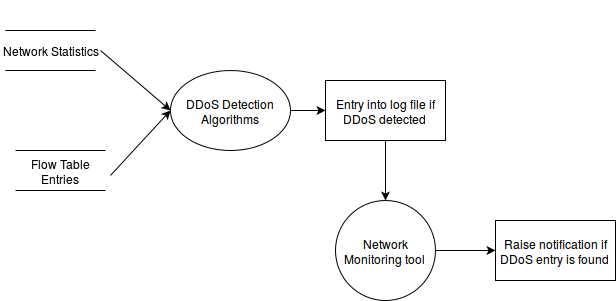
\includegraphics[scale=0.6]{dataflow0.png}
\caption{Level 0 Data Flow Diagram}
\end{center}
\end{figure}

\item
\textbf{Level 1 Data Flow Diagram :}
\newline
\begin{figure}[h]
\begin{center}
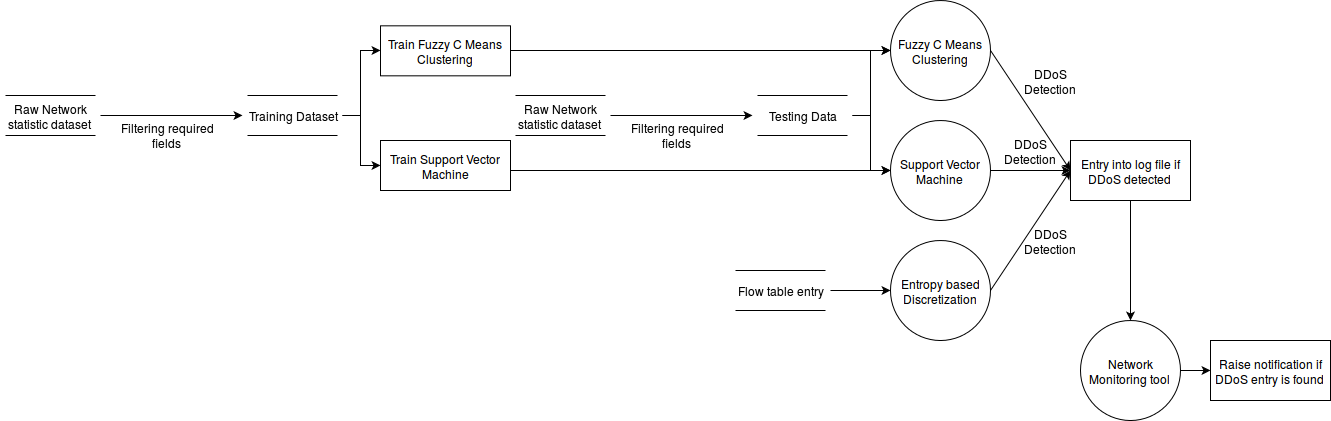
\includegraphics[scale=0.4]{dataflow1.png}
\caption{Level 1 Data Flow Diagram}
\end{center}
\end{figure}
\end{enumerate}

\newpage
\subsection{Activity Diagram}
\begin{figure}[h]
\begin{center}
\includegraphics[scale=0.5]{activity.png}
\caption{Activity Diagram}
\end{center}
\end{figure}

\subsection{Non Functional Requirements}
\begin{enumerate}
\item
\textbf{Interface Requirements}
\begin{enumerate}
\item OpenFlow Protocol :
\newline
Provides a medium for the SDN controller to direct traffic along the switches within the network.

\item Northbound API's :
\newline
Allow the SDN controller to communicate between services and applications running over the network owing to programmatic nature of SDN.

\item Southbound API's :
\newline
Allow the SDN controller to communicate between the network devices within the network.
\end{enumerate}

\item
\textbf{Software Quality Attributes}
\begin{enumerate}
\item Correctness:
\newline
The correctness of our product would depend upon the accuracy with which either of the application would detect the attack. For this purpose both applications must be trained in the network which they would monitor to generate the necessary constant values needed for their execution.

\item Availability:
\newline
As long as the network is up and running, this service would be also be available continuously monitoring the network for any anomalies.

\newpage
\item Usability: 
\newline
As and when a DDoS attack is detected, a simple notification is sent to the network administrative team. It does not disrupt their normal work flow or involve using complex application for monitoring purposes. Hence no specific training of the user is needed for using this system. 

\item Portability: 
\newline
Portability is restricted i.e. both applications must be given prior training before being deployed in a network. Thus the system being used in one enterprise cannot be used in another enterpise owing to the fact that the network traffic would vary from enterprise to enterprise such that normal traffic in one could be classified as attack traffic in another enterprise. Hence training in the network is of utmost importance.
\end{enumerate}
\end{enumerate}

\subsection{State Diagram}
\begin{figure}[h]
\begin{center}
\includegraphics[scale=0.6]{state.png}
\caption{State Diagram}
\end{center}
\end{figure}
\newpage

\AddToShipoutPictureBG*{%
\begin{tikzpicture}[overlay,remember picture]
\draw[line width=1.5pt]
    ($ (current page.north west) + (0.7cm,-0.7cm) $)
    rectangle
    ($ (current page.south east) + (-0.7cm,0.7cm) $);
\draw[line width=1.5pt]
    ($ (current page.north west) + (0.9cm,-0.9cm) $)
    rectangle
    ($ (current page.south east) + (-0.9cm,0.9cm) $);
\end{tikzpicture}
}
\chapter{Detailed Design Document}
\thispagestyle{empty}
\newpage
\section{Architectural Design}
\begin{figure}[h]
\begin{center}
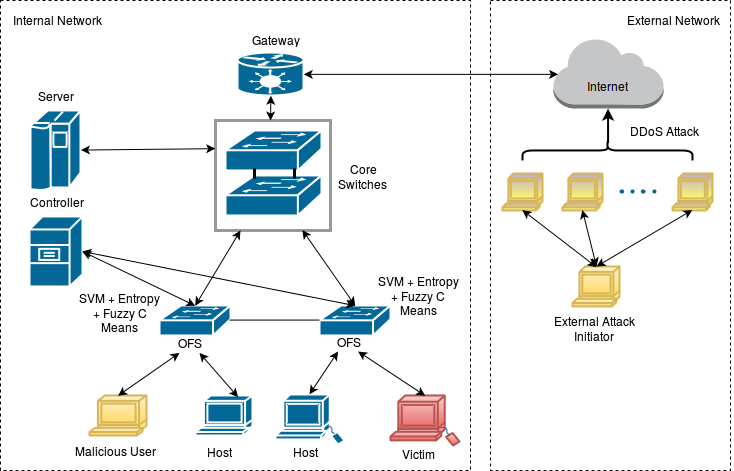
\includegraphics[scale=0.6]{architecture.png}
\caption{System Architecture}
\label{Architecture}
\end{center}
\end{figure}

During normal state of communication between two users in the network, the first packet is transmitted from the host to it's nearby switch. Initially the switch does not have any entry in its flow table as to where it should forward the incoming packet, hence the default route is to forward the packet to the controller. The controller then dictates the switch to forward the packet to the respective destination port. Along with this the controller also makes an entry in the flow table of the switch for the particular source and destination such that the future packets with the same source and destination are forwarded directly without any intervention of the controller.

This helps in reducing the time taken for communication between source and destination systems. After a particular interval of time the flow table entries are flushed and the process is repeated all over again.

The system is designed to detect two types of DDoS attacks namely :-
\begin{enumerate}
\item
Internal DDoS attack

\item
External DDoS attack
\end{enumerate}

In the first case, i.e. internal DDoS attack, the malicious user and the victim are located within the software defined network. 
whereas in external DDoS attack the host machine is from a different network. In both cases losses generated are immense.

The malicious machine can now launch attacks at two different points, one being the controller which would result in downfall of entire enterprise network incase there aren't any secondary controllers available, or the second point of attack could be one of host machines. 

In case of the attack point being the controller, the attack is generated by spoofing the source and destination ip address so that it does not match any flow table entry and hence must make a trip to the controller, this would burden the controller and thereby render its services unavailable. To overcome this issue, SVM monitors the rate of incoming packets and classifies it as normal traffic or attack traffic, similarly Entropy based mechanism would find a drop in the entropy in the network owing to the large number of same class of packets hence would be able to detect the DDoS attack, and Fuzzy C Means clustering would assign a membership value closer to "1" near the core switch since all packets are being directed towards the controller and thus would be able to detect a DDoS attack.

Another method of generating an attack would be by generating a multitude of requests at the host thereby rendering the system void of performing any other operations. This type of attack is also solved along similar guidelines such that SVM would monitor the rate of incoming packets and Entropy based mechanism would monitor the entropy of the network which would drop due to large number of same class of packets, similarly Fuzzy C Means, running on the edge switches would be able to place the incoming packets in the attack cluster thereby detecting a DDoS attack.

Hence, a comparison can be deduced as to which method would generate a result instantaneously and with higher accuracy.

Once the attack is detected by any of the applications an entry is made into the log file of the respective switch, which is constantly monitored by the network monitoring tool which on finding the entry raises a notification to the network admnistrative team. Further it is the responsibility of the network administrative team to take preventive measures to eliminate any damage that could be caused by an impending full fledged DDoS attack.

\section{Data Design}
\subsection{Dataset Description}
For the purpose of detection, all three algorithms use some form of data on which computation is performed and results are predicted. In case of Support Vector Machine the dataset consists of the network statistics, which have been converted to a "csv" file with limited fields using a terminal based tool "tshark".
\newline

The fields present in the dataset have been shown in table 2.1
\begin{table}[h]
\begin{center}
\begin{tabular}{|p{3cm}|p{3cm}|p{4cm}|p{3.5cm}|p{4cm}|}
\hline 
\textbf{Packet Interval} & \textbf{Source IP} & \textbf{Destination IP} & \textbf{Protocol} \\ 
\hline 
0.000300000 & 192.168.1.14 & 192.168.1.11 & 1 \\ 
\hline
\end{tabular} 
\end{center}
\caption{Dataset Fields - Support Vector Machine}
\end{table}

\begin{enumerate}
\item
\textbf{Packet Interval :}
\newline
Time interval between two incoming packets

\item
\textbf{Source IP :}
\newline
The source ip address of the sender machine.

\item
\textbf{Destination IP :}
\newline
The destination ip address of the receiver machine.

\item
\textbf{Protocol}
\newline
Protocol of the incoming packet.
\end{enumerate}

This dataset is again categorized into attack traffic dataset and normal traffic dataset, which can be shown in table 2.2 and 2.3, wherein the most standout variation is the packet interval field between normal traffic and attack traffic.
\begin{table}[h]
\begin{center}
\begin{tabular}{|p{3cm}|p{3cm}|p{4cm}|p{3.5cm}|p{4cm}|}
\hline 
\textbf{Packet Interval} & \textbf{Source IP} & \textbf{Destination IP} & \textbf{Protocol} \\ 
\hline 
0.000300000 & 192.168.1.14 & 192.168.1.11 & 1 \\ 
\hline
0.000100000 & 192.168.1.12 & 192.168.1.11 & 1 \\ 
\hline
0.000200000 & 192.168.1.13 & 192.168.1.11 & 6 \\ 
\hline
\end{tabular} 
\end{center}
\caption{Attack Dataset Fields - Support Vector Machine}
\end{table}

\newpage
\begin{table}[h]
\begin{center}
\begin{tabular}{|p{3cm}|p{3cm}|p{4cm}|p{3.5cm}|p{4cm}|}
\hline 
\textbf{Packet Interval} & \textbf{Source IP} & \textbf{Destination IP} & \textbf{Protocol} \\ 
\hline 
0.02000000 & 192.168.1.14 & 192.168.1.11 & 1 \\ 
\hline
0.01000000 & 192.168.1.14 & 192.168.1.11 & 1 \\ 
\hline
0.01000000 & 192.168.1.12 & 192.168.1.11 & 1 \\ 
\hline
\end{tabular} 
\end{center}
\caption{Normal Dataset Fields - Support Vector Machine}
\end{table}

Similar datasets are created during runtime using the packet capturing tool "tshark" and the classification is carried out on the same.
\newline

In case of Fuzzy C Means clustering, the nature of datasets used are the same. The only difference is the number of fields used. For Fuzzy C Means only the packet interval field is used to generate clusters and assign membership values to each packet. Also like SVM, Fuzzy C Means uses two datasets i.e. attack traffic and normal traffic for training the model, using the packet capturing tool "tshark", again which is stored in a csv file format. The training dataset appears to be like the one showed in table 2.4 and 2.5

\begin{table}[h]
\begin{center}
\begin{tabular}{|p{3cm}|}
\hline 
\textbf{Packet Interval} \\ 
\hline 
0.000300000 \\ 
\hline
0.000100000 \\ 
\hline
0.000200000 \\ 
\hline
\end{tabular} 
\end{center}
\caption{Attack Dataset Fields - Fuzzy C Means clustering}

\begin{center}
\begin{tabular}{|p{3cm}|}
\hline 
\textbf{Packet Interval} \\ 
\hline 
0.02000000 \\ 
\hline
0.01000000 \\ 
\hline
0.01000000 \\ 
\hline
\end{tabular} 
\end{center}
\caption{Normal Dataset Fields -Fuzzy C Means clustering}
\end{table}

However, unlike SVM and Fuzzy C Means that use packet level statistics for classification and clustering, Entropy based discretization uses the flow table entries residing in the switch to perform its computation. The flow table entries are dumped into a file during each time interval, which is then looked up by the entropy based application to detect what is the entropy of the network and accordingly detect whether a DDoS attack has been launched or not.
\newline

\newpage
Sample flow entry :
\newline
$cookie=0x0, duration=240.478s, table=0, n\_packets=21975265, n\_bytes=2153575970, idle\_timeout=60, idle\_age=0, priority=65535,icmp,in\_port=2,vlan\_tci=0x0000,dl\_src=4a:06:64:e9:ef:f0,dl_dst=f2:57:bd:4c:19:28,nw\_src=10.0.0.2,nw\_dst=10.0.0.1,nw\_tos=0,icmp\_type=0,icmp\_code=0 actions=output:1$
\newline

wherein the fields used during processing are:
\begin{enumerate}
\item
\textbf{$n\_packets$ :}
\newline
The total number of packets transitted by the switch having the same flow details.

\item
\textbf{$protocol$ :}
\newline
The protocol of the incoming packets.

\item
\textbf{$nw\_src$ :}
\newline
Source IP address

\item
\textbf{$nw\_dst$ :}
\newline
Destination IP address
\end{enumerate}
\newpage

\AddToShipoutPictureBG*{%
\begin{tikzpicture}[overlay,remember picture]
\draw[line width=1.5pt]
    ($ (current page.north west) + (0.7cm,-0.7cm) $)
    rectangle
    ($ (current page.south east) + (-0.7cm,0.7cm) $);
\draw[line width=1.5pt]
    ($ (current page.north west) + (0.9cm,-0.9cm) $)
    rectangle
    ($ (current page.south east) + (-0.9cm,0.9cm) $);
\end{tikzpicture}
}
\chapter{Project Implementation}
\thispagestyle{empty}
\newpage

\section{Introduction}
There was always an option to implement the project by creating a Software Defined Network in a  single system using network simulator called Mininet. But doing this would have decreased the quality of the project and our commitment that the solution can be used in real world deployment. In order to validate the effectiveness of the solution in real time environment we decided to deploy our own Software Defined Network on a small scale. This deployment was a challenge in itself as it is a new technology which is not well matured.

\section{Methodologies}
\subsection{Support Vector Machine}

\subsection{Entropy based discretization}

\subsection{Fuzzy C Means clustering}
\begin{algorithm}
\caption{Fuzzy C Means Clustering}
\begin{algorithmic}[1]
\Function{Calculate\_membership}{$cluster\_count, centroids, dataset$}
$membership = $
\Return $membership$
\EndFunction
\newline

\Function{Fuzzy}{$cluster\_count, centroids, training\_dataset$}
\State Let, $normal\_centroids[]$ and $attack\_centroids[]$ be new arrays
\State $ membership $ be a 2 dimensional list n*c
\newline
\hspace*{1cm}
where, 
\newline
\hspace*{1cm}
n = number of data points
\newline
\hspace*{1cm}
c = number of centroids
\State $ membership\_df $ be a dataframe representing the 2 dimensional $membership$ list
\State $training\_data = pandas.read\_csv(training\_dataset)$

\While{$True$}
\State $old\_membership = membership$
\State $old\_membership\_df = membership\_df$
\EndWhile
\For{$j = 1$ to ${n_2}$}
\State $R[i] = A[q + j]$
\EndFor
\State $L[{n_1} + 1] =  \infty $
\State $R[{n_2} + 1] =  \infty $
\State $i = 1$
\State $j = 1$
\For{$k = p$ to $r$}
\If {$L[i] < R[j]$}
\State $A[k] = L[i]$
\State $i = i + 1$
\ElsIf {$L[i] > R[j]$}
\State $A[k] = R[j]$
\State $j = j + 1$
\Else
\State $A[k] = - \infty$ \Comment{We mark the duplicates with the largest negative integer}
\State $j = j + 1$
\EndIf
\EndFor
\EndFunction

\end{algorithmic}
\end{algorithm}

\newpage
\AddToShipoutPictureBG*{%
\begin{tikzpicture}[overlay,remember picture]
\draw[line width=1.5pt]
    ($ (current page.north west) + (0.7cm,-0.7cm) $)
    rectangle
    ($ (current page.south east) + (-0.7cm,0.7cm) $);
\draw[line width=1.5pt]
    ($ (current page.north west) + (0.9cm,-0.9cm) $)
    rectangle
    ($ (current page.south east) + (-0.9cm,0.9cm) $);
\end{tikzpicture}
}
\chapter{Software Testing}
\thispagestyle{empty}
\newpage


\section{Type of Testing Used}
\begin{itemize}
\item Unit Testing
\item Integration Testing
\item System Testing
\item Positive Testing
\item Negative Testing
\end{itemize}


\section{Test Cases and Test Results}

\begin{enumerate}
\item\begin{flushleft}
Unit Testing 
\end{flushleft} 
	\begin{tabular}{|p{1cm}|p{3cm}|p{2.6cm}|p{2.5cm}|p{2.5cm}|}
	\hline 
	\textbf{Unit} & \textbf{Description} & \textbf{Scenario} & \textbf{Expected Output} & 		\textbf{Generated Output}\\ 
	\hline
	
	SVM & Attack Traffic & Attack has occured & Alert generation & Alert Generated\\
	\hline
	
	SVM & Normal Network Traffic & SDN functioning in normal mode & No alert generation & Alert is not Generated \\
	\hline
	
	EBD & Attack Traffic & Attack has occured & Alert generation & Alert Generated\\
	\hline
	
	EBD & Normal Network Traffic & SDN functioning in normal mode & No alert generation & Alert is not Generated \\
	\hline
	
	FCM & Attack Traffic & Attack has occured & Alert generation & Alert Generated\\
	\hline
	
	FCM & Normal Network Traffic & SDN functioning in normal mode & No alert generation & Alert is not Generated \\
	\hline
	
	\end{tabular}
	\linebreak
	
\item \begin{flushleft}
Integration Testing 
\end{flushleft} 
	\begin{tabular}{|p{3.5cm}|p{2.9cm}|p{2.5cm}|p{2.5cm}|}
	\hline 
	\textbf{Description} & \textbf{Scenario} & \textbf{Expected Output} & \textbf{Generated 		Output}\\ 
	\hline

	All three algorithms are running simultaneously and attack traffic in the network & Attack has occured & Alert generation & Alert Generated\\
	\hline
	
	All three algorithms are running simultaneously and Normal traffic in the network & SDN functioning in normal mode & no alert generation & Alert is not Generated\\
	\hline
	
	\end{tabular}
	\linebreak
\newpage	
\item \begin{flushleft}
System Testing 
\end{flushleft} 
	\begin{tabular}{|p{3.5cm}|p{2.9cm}|p{2.5cm}|p{2.5cm}|}
	\hline 
	\textbf{Description} & \textbf{Scenario} & \textbf{Expected Output} & \textbf{Generated 		Output}\\ 
	\hline
	
	Time span between attack detection and alert generation & Attack has occured & Instantaneous alert generation & Alert generated within 1 sec.\\
	\hline
	
	Normal Network Traffic & SDN functioning in normal mode & No alert generation & Alert is not Generated\\
	\hline
	
	\end{tabular}
	
	
\item \begin{flushleft}
Positive Testing 
\end{flushleft} 
	\begin{tabular}{|p{3.5cm}|p{2.9cm}|p{2.5cm}|p{2.5cm}|}
	\hline 
	\textbf{Description} & \textbf{Scenario} & \textbf{Expected Output} & \textbf{Generated 		Output}\\ 
	\hline
	
	Attack Traffic & Attack has occured & Alert generation & Alert Generated\\
	\hline
	
	\end{tabular}
	\linebreak
	
\item \begin{flushleft}
Negative Testing 
\end{flushleft} 
	\begin{tabular}{|p{3.5cm}|p{2.9cm}|p{2.5cm}|p{2.5cm}|}
	\hline 
	\textbf{Description} & \textbf{Scenario} & \textbf{Expected Output} & \textbf{Generated 		Output}\\ 
	\hline
	
	 Normal Network Traffic & SDN functioning in normal mode & No alert generation & Alert is not Generated \\
	 \hline	
	
	\end{tabular}

\end{enumerate}


\newpage

\AddToShipoutPictureBG*{%
\begin{tikzpicture}[overlay,remember picture]
\draw[line width=1.5pt]
    ($ (current page.north west) + (0.7cm,-0.7cm) $)
    rectangle
    ($ (current page.south east) + (-0.7cm,0.7cm) $);
\draw[line width=1.5pt]
    ($ (current page.north west) + (0.9cm,-0.9cm) $)
    rectangle
    ($ (current page.south east) + (-0.9cm,0.9cm) $);
\end{tikzpicture}
}
\chapter{Results}
\thispagestyle{empty}
\newpage
\section{Screenshots}
\begin{figure}[h]
\centering
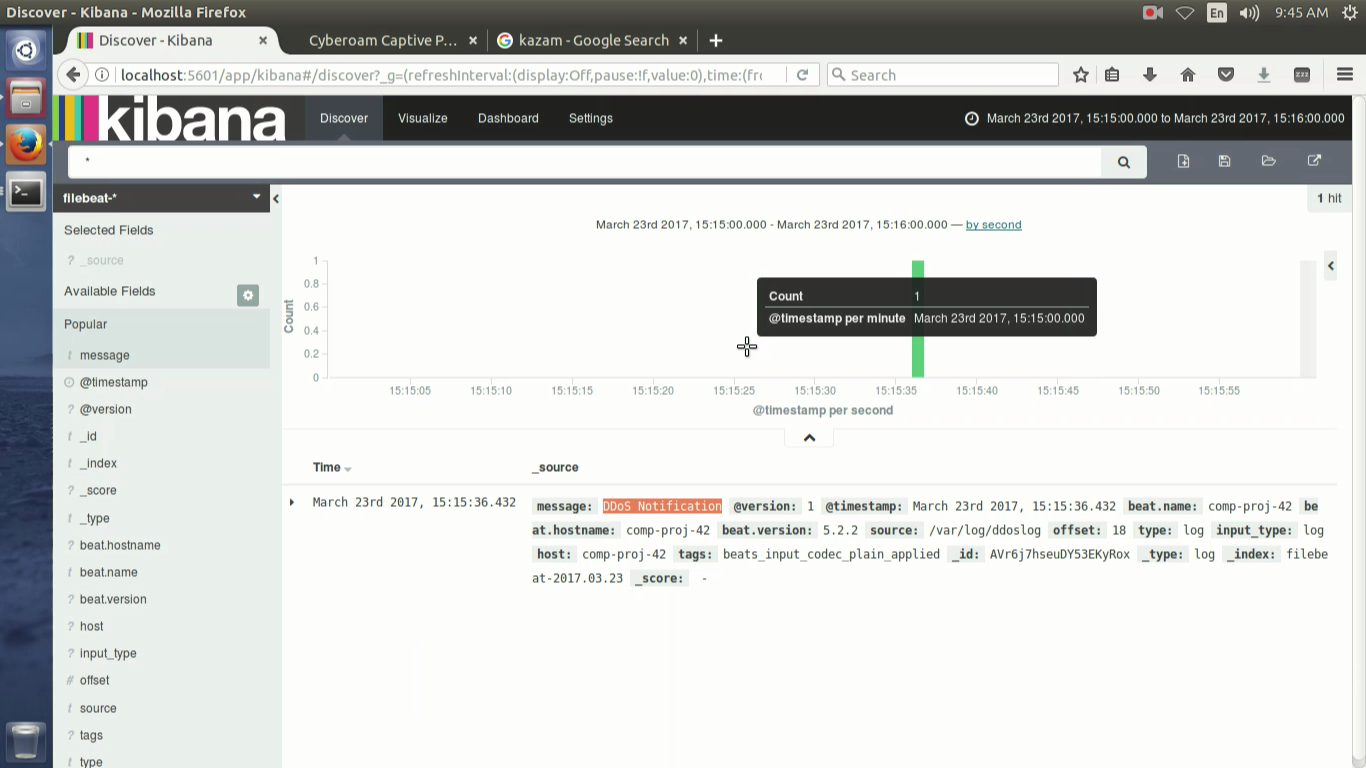
\includegraphics[scale=0.3]{Kibana.png}
\caption{Kibana Dashboard}
\end{figure}

\begin{figure}[h]
\centering
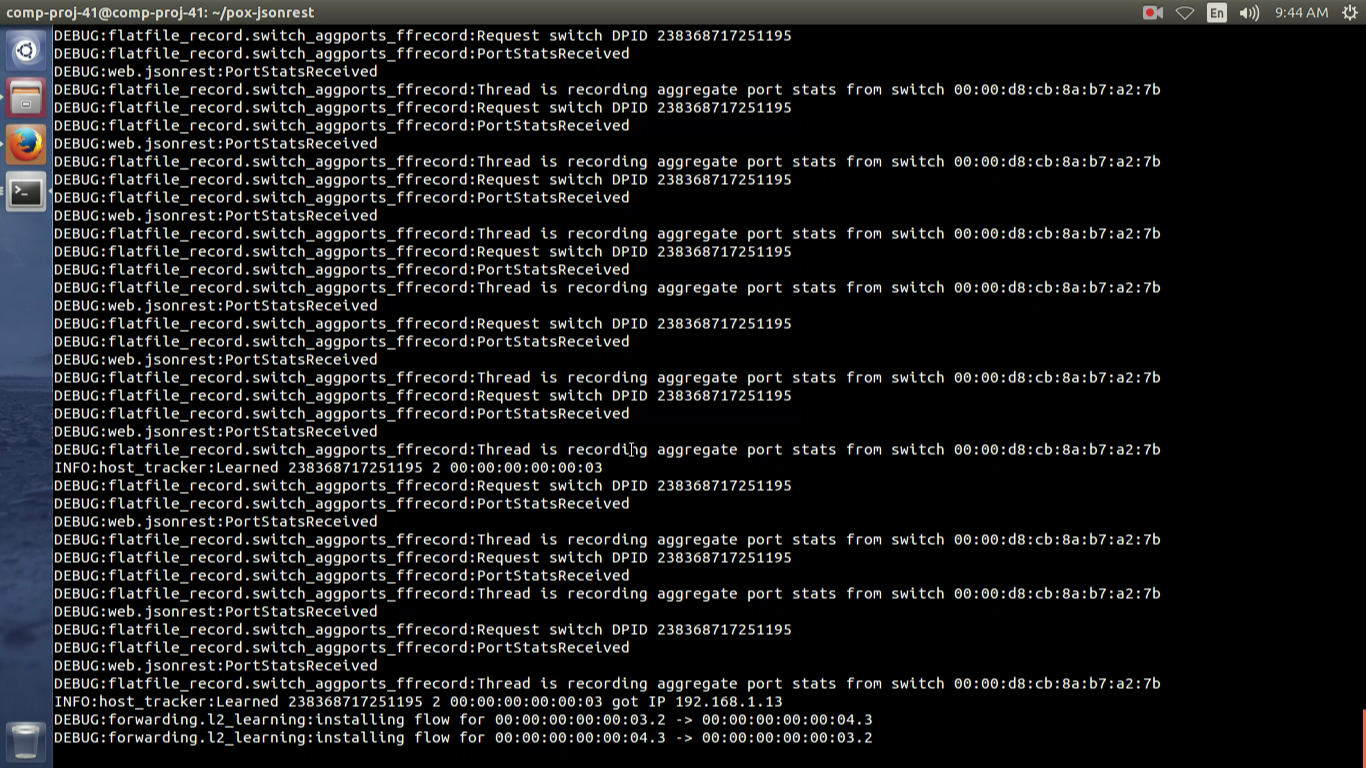
\includegraphics[scale=0.3]{Controller.png}
\caption{POX Controller Output}
\end{figure}

\newpage

\section{Output}

\begin{figure}[h]
\centering
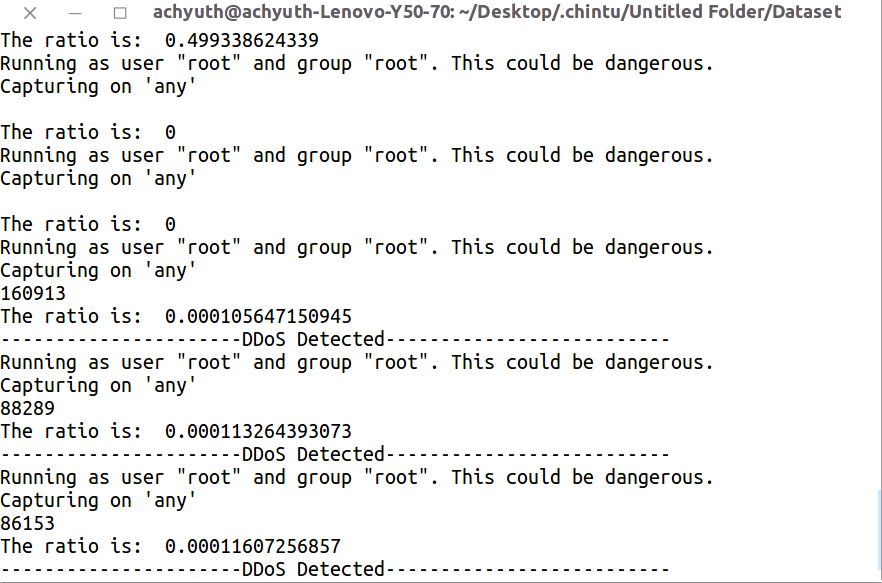
\includegraphics[scale=0.4]{SVMOutput.png}
\caption{SVM Algorithm Output}
\end{figure}



\begin{figure}[h]
\centering
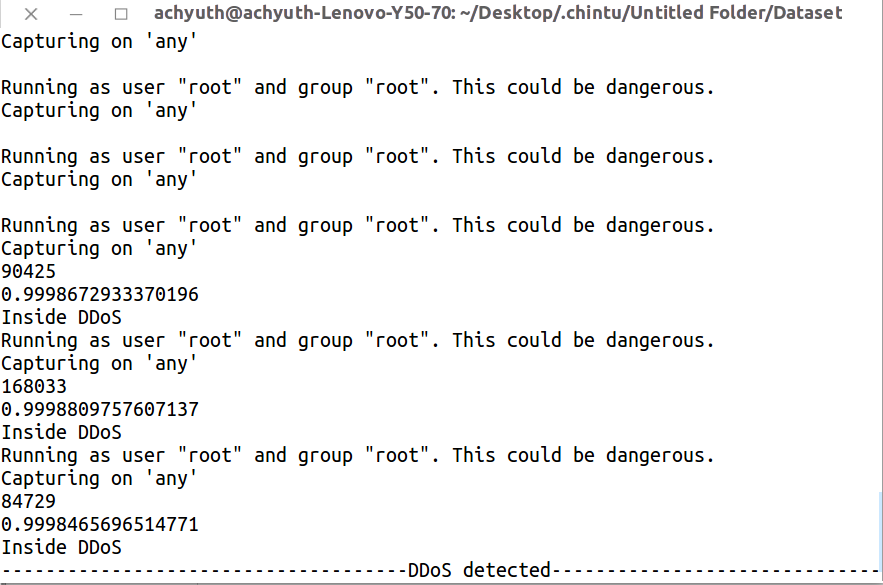
\includegraphics[scale=0.4]{FuzzyOutput.png}
\caption{Fuzzy C-Means Algorithm Output}
\end{figure}



\newpage

\AddToShipoutPictureBG*{%
\begin{tikzpicture}[overlay,remember picture]
\draw[line width=1.5pt]
    ($ (current page.north west) + (0.7cm,-0.7cm) $)
    rectangle
    ($ (current page.south east) + (-0.7cm,0.7cm) $);
\draw[line width=1.5pt]
    ($ (current page.north west) + (0.9cm,-0.9cm) $)
    rectangle
    ($ (current page.south east) + (-0.9cm,0.9cm) $);
\end{tikzpicture}
}
\chapter{Deployment and Maintenance}
\thispagestyle{empty}
\newpage
\section{Installation and un-installation}

\section{User Help}
\newpage

\AddToShipoutPictureBG*{%
\begin{tikzpicture}[overlay,remember picture]
\draw[line width=1.5pt]
    ($ (current page.north west) + (0.7cm,-0.7cm) $)
    rectangle
    ($ (current page.south east) + (-0.7cm,0.7cm) $);
\draw[line width=1.5pt]
    ($ (current page.north west) + (0.9cm,-0.9cm) $)
    rectangle
    ($ (current page.south east) + (-0.9cm,0.9cm) $);
\end{tikzpicture}
}
\chapter{Conclusion and Future Scope}
\thispagestyle{empty}
\newpage
The report introduces the problems faced in the Software Defined Networking Environment such as DDoS,
application layer attack, brute force and phishing. As the SDN Controller seperates the Application layer and 
the Data flow plane in the network, it becomes a point of vulnerability for the attackers to target by using 
such attacks.

DDoS attack when targetted on the controller can pose a huge impact on the whole network compromizing the system 
responsible for the Business logic. Thus it is very important to use a mechanism which can detect and mitigate such 
anomaly based attacks, we focus on the prior and not the later part of the mechanism.

There are several methods which can be used for the detection of DDoS such as use of neural networks, chaotic 
systems, filtering algorithms etc. Considering the advantages of Support Vector Machines, Entropy Based Discretization and Fuzzy C Means Clustering algorithms, we will be using them.

We then procede by stating the product features,user characteristics, system features, interfaces and quality 
attributes like correctness,usability etc. We also provide necessary diagramatic representations like the 
sequence diagram, use case diagram etc.

We then give a description of the system components, system architecture as well as the functioning of the whole
network environment. We also specify two cases of the DDoS attack scenarios namely, internal and external attacks and the method in which we detect the attack using the proposed algorithmic strategies. After the detection of the attack, the network administrator will be notified by the mechanism and a graphical interface would be provided for the administrator for finding the point of attack.

This project will be a step towards solving the security issues faced right now. This will be a challenging endevour for us as we try to incorporate concepts like networking, machine learning and data mining.  
\newpage

\AddToShipoutPictureBG*{%
\begin{tikzpicture}[overlay,remember picture]
\draw[line width=1.5pt]
    ($ (current page.north west) + (0.7cm,-0.7cm) $)
    rectangle
    ($ (current page.south east) + (-0.7cm,0.7cm) $);
\draw[line width=1.5pt]
    ($ (current page.north west) + (0.9cm,-0.9cm) $)
    rectangle
    ($ (current page.south east) + (-0.9cm,0.9cm) $);
\end{tikzpicture}
}
\SkipTocEntry\chapter{Bibliography}
\thispagestyle{empty}
\newpage
\begingroup
\renewcommand{\chapter}[2]{}
\begin{thebibliography}{9}
\bibitem{BasePaper1}
Diego Kreutz, Fernando M. V. Ramos, Paulo Verissimo, Christian Esteve Rothenberg, Siamak Azodolmolky, Steve Uhlig,
``Software-Defined Networking: A Comprehensive Survey",
Version 2.01,
8 Oct 2014

\bibitem{BasePaper2}
Open Networking Foundation, 
``Software-Defined Networking: The New Norm for Networks",
ONF white paper, 
April 13, 2012

\bibitem{BasePaper3}
Shiva Rowshanrad, Sahar Namvarasl, Vajihe Abdi, Maryam Hajizadeh, Manijeh Keshtgary,
``A survey on SDN, the future of networking",
in Journal of Advanced Computer Science and Technology,
pg 232-248,
2014

\bibitem{BasePaper4}
Rishikesh Sahay, Gregory Blanc, Zonghua Zhang, Herve Debar,
``Towards Autonomic DDoS Mitigation using Software Defined Networking",
Feb 2015,
http://www.internetsociety.org/doc/towards-autonomic-DDoS-mitigation-using-software-defined-networking

\bibitem{BasePaper5}
Seyed Mohammad Mousavi,
``Early Detection of DDoS Attacks in Software Defined Networks Controller",
2014

\bibitem{BasePaper6}
Shunsuke Oshima, Takuo Nakashima, Toshinori Sueyoshi,
``Early DoS/DDoS Detection Method using Short-term Statistics",
Presented at International Conference on Complex, Intelligent and Software Intensive Systems,
2010

\bibitem{BasePaper7} 
Kokila RT, S.Thamarai Selvi, Kannan Govindarajan,
``DDoS Detection and Analysis in SDN-based Environment Using Support Vector Machine Classifier",
presented at Sixth International Conference on Advanced Computing(ICoAC),
2014,

\bibitem{BasePaper8}
Xue Li, Dongming Yuan, Hefei Hu, Jing Ran, Shulan Li, 
``DDoS detection in SDN switches using support vector machine classifier",
in Joint International Mechanical, Electronic and Information Technology Conference, 
2015

\bibitem{BasePaper9} 
Rui Wang, Zhiping Jia∗, Lei Ju,
``An Entropy-Based Distributed DDoS Detection Mechanism in Software-Defined Networking",
in IEEE Trustcom/BigDataSE/ISPA,
DOI 10.1109/Trustcom.2015.389,
2015

\bibitem{BasePaper10}
T.Subbulakshmi, Dr. S. Mercy Shalinie, V.GanapathiSubramanian, K.BalaKrishnan, D. AnandKumar, K.Kannathal,
``Detection of DDoS Attacks using Enhanced Support Vector Machines with Real Time Generated Dataset",
in IEEE-ICoAC, 
2011

\bibitem{BasePaper11}
I Gde Dharma N., M. Fiqri Muthohar, Alvin Prayuda J. D., Priagung K., Deokjai Choi,
``Time-based DDoS Detection and Mitigation for SDN Controller",
Presented at APNOMS,
2015

\bibitem{BasePaper12}
Shibo Luo, Jun Wu, Jianhua Li,
``A Defense Mechanism for Distributed Denial of Service Attack in Software-Defined Networks",
Presented at Ninth International Conference on Frontier of Computer Science and Technology,
2015

\bibitem{BasePaper13}
K. Giotis, C. Argyropoulos, G. Androulidakis, D. Kalogeras, V. Maglaris,
``Combining OpenFlow and sFlow for an effective and scalable anomaly detection and mitigation mechanism on SDN environments",
2013, 
http://dx.doi.org/10.1016/j.bjp.2013.10.014

\bibitem{BasePaper14}
Seyed Mohammad Mousavi, Marc St-Hilaire,
``Early Detection of DDoS Attacks against SDN Controllers",
Presented at International Conference on Computing, Networking and Communications, Communications and Information Security
Symposium,
2015

\bibitem{BasePaper15}
P. K. Agrawal, B. B. Gupta, Satbir Jain,
``SVM Based scheme for Predicting Number of Zombies in a DDoS Attack",
Presented at European Intelligence and Security Informatics Conference,
2011

\bibitem{BasePaper16}
A. Ramamoorthi, T. Subbulakshmi, Dr. S. Mercy Shalinie,
``Real Time Detection and Classification of DDoS Attacks using Enhanced SVM with String Kernels",
in IEEE-International Conference on Recent Trends in Information Technology,
ICRTIT 2011,
June 2011

\bibitem{BasePaper17}
Ingo Steinwart, Andreas Christmann,
``Support Vector Machines",
Springer, 
2008

\bibitem{BasePaper18}
Alexander Gelbukh, Félix Castro Espinoza, Sofía N. Galicia-Haro,
``Nature-Inspired Computation and Machine Learning",
Springer,
2014
\end{thebibliography}
\endgroup
\newpage

\AddToShipoutPictureBG*{%
\begin{tikzpicture}[overlay,remember picture]
\draw[line width=1.5pt]
    ($ (current page.north west) + (0.7cm,-0.7cm) $)
    rectangle
    ($ (current page.south east) + (-0.7cm,0.7cm) $);
\draw[line width=1.5pt]
    ($ (current page.north west) + (0.9cm,-0.9cm) $)
    rectangle
    ($ (current page.south east) + (-0.9cm,0.9cm) $);
\end{tikzpicture}
}
\SkipTocEntry\chapter{Annexure A}
\thispagestyle{empty}
\newpage
\SkipTocEntry\section{IDEA Matrix}
\begin{table}[h]
\caption{IDEA Matrix}

\begin{center}
\begin{tabular}{|>{\bf}M{2.5cm}||>{\bf}M{2.5cm}||>{\bf}M{2.5cm}||>{\bf}M{2.5cm}|}
\hline
\rowcolor{lightgray}
I & D & E & A \\ \hline
\normalfont{Innovative} & \normalfont{Detect}  & \normalfont{Evaluate} & \normalfont{Associate} \\ \hline
\normalfont{Increase} & \normalfont{Decrease}  & \normalfont{Effective} & \normalfont{Acquire} \\ \hline
\normalfont{Investment} & \normalfont{Depict}  & \normalfont{Enhance} & \normalfont{Analyse} \\ \hline
\end{tabular}
\end{center}
\end{table}

\begin{center}
\begin{tabular}{|m{2cm}|m{7cm}|}
\hline
Innovative & Up till now, DDoS detection systems uses a single mechanism for its working. Here, the system will be using two mechanisms i.e. support vector machine, fuzzy c means clustering and entropy based discretization simultaneously which is \textbf{innovative}. \\

&\\

Increase & As the system will be using support vector machine, fuzzy c means clustering and entropy based discretization, efficiency of the system will \textbf{increase}. \\

&\\

Investment & As the system contains Software components only. So, \textbf{zero investment} is required to implement the system in already deployed software defined network. \\

\hline
\end{tabular}
\end{center}

\vspace*{1cm}
\begin{center}
\begin{tabular}{|m{2cm}|m{7cm}|}
\hline

Detect & The system will \textbf{detect} DDoS attack and raise notification to the network administrator team. \\

&\\

Decrease & The DDoS detection algorithm will \textbf{decrease} the possibility of false positive attack detection. \\

&\\

Depict & The system will \textbf{depict} appropriately whether the network traffic is normal or attack traffic. \\

\hline
\end{tabular}
\end{center}

\newpage
\begin{center}
\begin{tabular}{|m{2cm}|m{7cm}|}
\hline

Evaluate & An important part of the implementation is the \textbf{evaluation} of the rate of flow of packets per unit time. \\

&\\

Effective & The system analyses the traffic and detects the attack at runtime thus, increasing the \textbf{effectiveness}. \\

&\\

Enhance & The accuracy of the system will be \textbf{enhanced} by using an environment - specific training dataset for SVM and Fuzzy C Means. \\

\hline
\end{tabular}
\end{center}

\vspace*{1cm}
\begin{center}
\begin{tabular}{|m{2cm}|m{7cm}|}
\hline

Associate & The project is a step towards \textbf{association} and integration of next generation networking with advanced computing concepts like Machine Learning and Data Mining. \\

&\\

Acquire & The flow table containing the flow entries along with the information of the count of the packets is \textbf{acquired} from the SDN switches. \\

&\\

Analyse & The system will \textbf{analyse} the data acquired from the switches to perform the intended task of detecting the DDoS attack. \\

\hline
\end{tabular}
\end{center}
\newpage
\SkipTocEntry\section{Mathematical Model}
\SkipTocEntry\subsection{Mathematical Model}
{\setlength{\mathindent}{0cm}
\begin{equation}
S = \lbrace \lbrace I \rbrace ,\lbrace P \rbrace,\lbrace O \rbrace \rbrace
\end{equation}

\noindent
where,\\
$I =$ Input set,\\
$P = \lbrace P_{EBD}, P_{SVM}, P_{FCM} \rbrace$ Processing set, \\
$O =$ Output set

\SkipTocEntry\subsection{Input:}
{\setlength{\mathindent}{0cm}
\begin{equation}
I = \lbrace N \rbrace
\end{equation}

\noindent
where,\\
$N = \lbrace $ Network Statistics $ \rbrace $, \\
$F =\lbrace F_{i} \mid F_{i} \in T , \forall i$ $ F_{i} =$ Individual entry $ \rbrace$, \\
$T = \lbrace $ Flow Table $ \rbrace$, \\
$F \subseteq N$

\SkipTocEntry\subsection{Input for EBD:}

{\setlength{\mathindent}{0cm}
\begin{equation}
I_{EBD} = \lbrace U_{i} \mid U_{i} = ($ Source Address, Destination Address, Port no., Count$),  $ $ U_{i}  \subset F_{i} \rbrace
\end{equation}

\SkipTocEntry\subsection{Input for SVM:}

{\setlength{\mathindent}{0cm}
\begin{equation}
I_{SVM} = \lbrace V_{i} \mid V_{i} = ($ Source Address, Destination Address, Port no., Time, Protocol, Count$),  $ $ V_{i}  \subset F_{i} \rbrace
\end{equation}

\SkipTocEntry\subsection{Input for FCM:}

{\setlength{\mathindent}{0cm}
\begin{equation}
I_{FCM} = \lbrace V_{i} \mid V_{i} = ($Time$),  $ $ V_{i}  \subset F_{i} \rbrace
\end{equation}



\SkipTocEntry\subsection{Processing:}
$P_{EBD} $ $ (I_{EBD},$ $O_{EBD})$\\
$\lbrace$

\begin{enumerate}

\item 
{\setlength{\mathindent}{0cm}}
\begin{equation}
P_{i} = \frac{C_{i}}{N}
\end{equation}
where, \\ $c =$ counter, \\ $N = \sum_{i=0}^{n} C_{i}$, \\ $n =$ no. of entries.

\item 
{\setlength{\mathindent}{0cm}}
\begin{equation}
\varepsilon = \sum_{i=0}^{n} - P_{i} log P_{i}
\end{equation}

\newpage
\item 
\begin{equation}
(\lambda < \varepsilon) \rightarrow (\beta = 0)
\end{equation}
\begin{equation}
(\lambda > \varepsilon) \rightarrow (\beta = 1)
\end{equation}

\item  
\begin{equation}
O_{EBD} = \lbrace \beta \mid \beta \in (0,1) \rbrace
\end{equation}

\end{enumerate}

\noindent
$\rbrace$
\\


\noindent
$P_{SVM} $ $ (I_{SVM},$ $O_{SVM})$\\
$\lbrace$
\indent
Here, \\
\indent $\gamma$ , $c$, $x$, $x_{1}$, $x_{2}$, $b$ and $\overline{\omega}$ are constants.\\
\indent These values are calculated from Training Phase.\\
\indent Training of SVM is based on dataset used.


\begin{enumerate}

\item 
\begin{equation}
RBF = e^{-\gamma(\mid x_{1}-x_{2} \mid)+c}
\end{equation}
where, \\ $\gamma =$ width of boundries of hyperplane, \\ $c =$ soft margin parameter, \\ $x_{1}, $ $x_{2} =$ support vectors.


\item
\begin{equation}
y = \overline{\omega} * x + b
\end{equation}
where, \\ $x =$ support vector, \\ $b =$ boundary width, \\ $\overline{\omega} =$ libsvm.w().

\item
\begin{equation}
(y \leq -1) \rightarrow (\alpha = 1)
\end{equation}
\begin{equation}
(y \geq 1) \rightarrow (\alpha = 0)
\end{equation}

\item
\begin{equation}
O_{SVM} = \lbrace \alpha \mid \alpha \in (0, 1) \rbrace
\end{equation}

\end{enumerate}

$\\ \rbrace$

\newpage

\noindent
$P_{FCM} $ $ (I_{FCM},$ $O_{FCM})$\\
$\lbrace$
\indent
Here, \\
\indent $m$ is a constant.\\
\indent This value is used for the calculation of the membership values of the data points.\\


\begin{enumerate}

\item 
\begin{equation}
u_{ij} = \frac{\frac{-2}{d_{ij}^{m-1}}}{\sum_{i=1}^{c}{{d_{ij}^{m-1}}}}
\end{equation}
where, \\ $d_{ij}^{m-1}=$ distance of the $i^{th}$ point from the $j^{th}$ centroid\\
$c =$ centroid.

\item
\begin{equation}
C_{i} = \frac{\sum_{j=1}^{n}u_{ij}^{m}X_{ij}}{\sum_{n}^{j=1}u_{ij}^{m}}
\end{equation}
where, \\ $u_{ij}^{m}=$ membership value of the data point. \\
$X_{ij}=$ data point. 


\item
\begin{equation}
(X \geq \lambda) \rightarrow (w = 1)
\end{equation}
\begin{equation}
(X < \lambda) \rightarrow (w = 0)
\end{equation}


\item
\begin{equation}
O_{FCM} = \lbrace w \mid w \in (0, 1) \rbrace
\end{equation}

\end{enumerate}

$\\ \rbrace$




\SkipTocEntry\subsection{Output:}

\begin{equation}
O_{EBD} = \lbrace z \mid \exists z, z \in \beta \rbrace
\end{equation}
\begin{equation}
O_{SVM} = \lbrace x \mid \exists x, x \in \alpha \rbrace
\end{equation}
\begin{equation}
O_{FCM} = \{w \mid \exists w, w\in \gamma \rbrace
\end{equation}


\begin{equation}
O_{system} = \lbrace O_{EBD} \cup O_{SVM} \cup O_{FCM} \rbrace
\end{equation}

\SkipTocEntry\subsection{Feasibility Study}
To check the feasibility of Entropy Based Discretization, Support Vector Machine abd Fuzzy C-Means Clustering:
\newline Since, the problem we solve is essentially a decision problem, it is very essential to analyse the running time of the system. The strategies used in the system are SVM, Entropy Based Discretization and Fuzzy C-Means clustering. It is well known that EBD takes O(n) running time thus is in P.\\
\newline
Now, we will find the computational complexity for Support Vector Machines:\\
For a training dataset D=\{$x_i$,$y_i$\} where, $x_i$ $\in$ $\Re$ and $y_i$ $\in$ \{+1,-1\}.\\
The Support Vector Machine classifies with seperating hyperplane given by:\\

\begin{equation}
D(x)=w^Tx+b
\end{equation}

The above equation is obtained by:
\begin{equation}
L=\frac{1}{2} \emph{w}^2 - \sum_{}^{} \zeta_i
\end{equation}

s.t. $y_i$($w^T$ $x_i$ + b) $\geq$ 1 - $\zeta_i$, $\zeta_i$ $>$ 0 for i=1,2,...,m \\
\newline The problem is equivalent to the problem:\\
\begin{equation}
Max L(\alpha)= \sum_{i=1}^{M} \alpha_i - \frac{1}{2} \sum_{i=1}^{m}\sum_{j=1}^{m} y_iy_j\alpha_i\alpha_jk(x_i,y_j)
\end{equation}

where k($x_1$,$y_1$) is the Mercer's Kernel which is used for the 
Dimensional reduction.\\
\newline We will use the following four steps to prove the complexity of the SVM problem:
\begin{enumerate}
\item
Denote the problem as \textbf{$\pi$} and justify that it is in NP.
\item
Selecting a known problem \textbf{$\pi$'} which is in NP.
\item
Construct a tranformation function from $\pi$' to $\pi$.
\item
Prove that the transformation function is polynomial.
\end{enumerate}
\begin{itemize}

\item
\textbf{The SVM Problem ($\pi$)}
\newline For a set of kernels A=\{$k_1,k_2,...,k_n$\} the objective function can be written as:\\

\begin{equation}
C(A')=	\Big[\sum_{k \in A'}^{}\Big(\frac{1}{q}\Big[\sum_{i=1}^{m} \alpha_i - \frac{1}{2q^2} \sum_{i=1}^{m}\sum_{j=1}^{m}y_iy_jk(x_i,x_j)\alpha_i\alpha_j\Big]\Big)^2- B\Big]^2
\end{equation}	
\newline 

Where, we have to find a subset A' $\subseteq$ A of size q to minimize the cost. The cost function is used for reaching a bound B using set of Kernels, dataset and the Support Vectors.\\
\item
\textbf{SVM is in NP}
\newline To justify that SVM is in NP, we have to show that any instance of the problem can be guessed and verified to solve or not in polynomial time.\\
Let there be a function, that accepts q which returns random indices of q from the set of kernels and computes the most optimum solution A'. As the set of Lagrange Multipliers, dataset, q and Bound is known beforehand, the kernel evaluations are the only states.  These kernel evaluations are merely dot products among the directional vectors. The evaluation is polynomial and thus the instances A' can easily be generated and verified. Hence, we can say that SVM is in NP.
\item
\textbf{Selecting a known NP-Complete Problem ($\pi$')}
\newline The known problem selected is the subset problem which is as defined,\\
Given a set A, a size s(a) for each a $\in$ A and an integer B. Is there an A' $\subseteq$ A such that the sum of the sizes of the elements in is exactly B?\\
\item
\textbf{Transformation function $\mathcal{F}$ from $\pi$' to $\pi$}
\newline The transformation function $\mathcal{F}$ should map every instance (\emph{I}) such that every instance of "yes" in $\pi$ should map to the corresponding instance (\emph{I'}) in $\pi$'.\\
First, A stands for set of kernels: A=\{$A_1,A_2,...,A_n$\} \\
To compute B the following procedure should be followed: \\
\begin{enumerate}
\item
Solve SVM for all k $\in$ A with dataset D.
\item
Use the kernel $k^*$ and the dataset D to find the most optimal solution for SVM denoted by $M^* = (V^*,k^*)$
\item 
Now, B can be calculated by:- 
\begin{equation}
B = \Big[\sum_{i=1}^{m} \alpha_i - \frac{1}{2}\sum_{i=1}^{m}\sum_{j=1}^{m}y_iy_jk^*(x_i,x_j)\alpha_i,\alpha_j\Big]^2
\end{equation} 
\item
Finally we have to calculate the size function s(a)=s(k $\in$ A) which can be done by the formula:- \\
\begin{equation}
s(k) = \Big[\big(\frac{1}{q}\sum_{i=1}^{m}\alpha_i - \frac{1}{2q^2}\sum_{i=1}^{m}\sum_{j=1}^{m}y_iy_jk(x_i,x_j)\alpha_i\alpha_j\Big)\Big]^2
\end{equation}
Where, s(k) is the value of the objective function. 
\end{enumerate} 
Now, we know that $\sum_{k \in A}^{}s(k)=B$ when $k^*(x_i,x_j)=\frac{1}{q^2}\sum_{k \in A'}^{},(k_i,k_j)$ \\
This can be written in the form: \\
\begin{equation}
\Big[\sum_{k \in A'}^{}\Big(\frac{1}{q}\sum_{i=1}^{m}\alpha_i - \frac{1}{2q^2}\sum_{i=1}^{m}\sum_{j=1}^{m}y_iy_jk(x_i,x_j)\alpha_i\alpha_j\Big) \Big]^2 = \Big[\sum_{i=1}^{m} \alpha_i - \frac{1}{2}\sum_{i=1}^{m}\sum_{j=1}^{m}y_iy_jk^*(x_i,x_j)\alpha_i\alpha_j\Big]^2
\end{equation}
Taking squared-root and using summation property, \\
\begin{equation}
\sum_{k \in A'}\Big(\frac{1}{q}\sum_{i=1}^{m}\alpha_i\Big)+\sum_{k \in A'}^{}\Big[-\frac{1}{2q^2}\sum_{i=1}^{m}\sum_{j=1}^{m}y_iy_jk(x_i,x_j)\alpha_i\alpha_j\Big] = \sum_{i=1}^{m}\alpha_i-\frac{1}{2}\sum_{i=1}^{m}\sum_{j=1}^{m}y_iy_jk^*(x_i,x_j)\alpha_i\alpha_j
\end{equation}
Simplifying the equation,
\begin{equation}
\sum_{k \in A'}\Big[\frac{1}{q^2}\sum_{i=1}^{m}\sum_{j=1}^{m}y_iy_jk(x_i,x_j)\alpha_i\alpha_j\Big] = \sum_{i=1}^{m}\sum_{j=1}^{m}y_iy_jk^*(x_i,x_j)\alpha_i\alpha_j
\end{equation}
Substituting $\Delta_{i,j}$ = $y_iy_j\alpha_i\alpha_j$ for simplification purpose \\
\begin{equation}
\sum_{k \in A'}\Big[\frac{1}{q^2}\sum_{i=1}^{m}\sum_{j=1}^{m}\Delta_{i,j}k(x_i,x_j)\Big] = \sum_{i=1}^{m}\sum_{j=1}^{m}\Delta_{i,j}k^*(x_i,x_j)
\end{equation}
Cancelling common terms,
\begin{equation}
\frac{1}{q^2}\sum_{k \in A'}{}k(x_i,x_j)=k^*(x_i,x_j)
\end{equation}
Thus, 
\begin{equation}
\sum_{k \in A'}s(k) = B \leftrightarrow k^*(x_i,x_j) = \frac{1}{q^2}\sum_{k \in A'}k(x_i,x_j)
\end{equation}
This implies that the transformed subset problem is equivalent to SVM classification using an optimum kernel. Thus, for every instance of (\emph{I')} if the answer is "yes" the answer can be mapped for the instance  of (\emph{I}). \\
\item
\textbf{$\mathcal{F}$ is a polynomial Transformation}
\newline The last part is to prove that the $\mathcal{F}$ is polynomial. The most expensive step is to find the Boundary (B) in the training phase.\\
This problem of training is a quadratic problem(QP). This problem can be seen as a convex problem. There are methods like Ellipsoids to solve it in polynomial time. 
It is also known that QP can be solved in O($m^3$), for  SVM ``m'' is the number of input vectors. Therefore, $\mathcal{F}$ is a polynomial transformation. \\
\newline 

Now, we have to analyze the Fuzzy C-Means clustering.\\
the following are: the steps of the running of the FCM algorithm:
\begin{enumerate}
\item
Initializing the centroids for the cluster.
\item
Calculate the membership values of the data points for the initialized clusters.
\item
recalculate the centroids of the cluster.
\item
recalculate the membership values for every data point until the centroid values and the membership values do not change.
\end{enumerate}

The calculation of the membership values take place using the following equation:- 
\begin{equation}
u_{ij} = \frac{\frac{-2}{d_{ij}^{m-1}}}{\sum_{i=1}^{c}{{d_{ij}^{m-1}}}}
\end{equation}
And, the calculation of the centroid is done by the following equation:- 
\begin{equation}
C_{i} = \frac{\sum_{j=1}^{n}u_{ij}^{m}X_{ij}}{\sum_{n}^{j=1}u_{ij}^{m}}
\end{equation}

\newpage
\begin{enumerate}
\item
Fuzzy C-Means is a generalization of Hard C-Means or K-Means clustering algorithm. The clustering based algorithms are well known to fall under the NP-Hard type of problems.
\item
This is because, the clustering algorithms provide a global solution which causes them not to converge even for a large number of iterations. Thus, we have to limit the number of iterations that can take place.\\
\item
Also, there is no linear relationship between the point of convergence and the number of iterations. Therefore, we can not be certain that for a particular number of iterations the clustering will converge. This is analogous to the Halting probelm in the Turing machine which is well known to be a NP-Hard problem.
\item
The time complexity of FCM is O(nd$c^{2}$i) where, \\
n = Number of data points. \\
c = Number of clusters. \\
d = Number of dimensions. \\
i = Number of iterations. \\
\end{enumerate}
Thus, \\
SVM is NP-Complete, Entropy based mechanism is Polynomial and Fuzzy C-Means clustering is NP-Hard.\\
By Cook's Theorem, P $\in$ NP therefore, the proposed solution is NP-Hard. 
\end{itemize}
\newpage

\AddToShipoutPictureBG*{%
\begin{tikzpicture}[overlay,remember picture]
\draw[line width=1.5pt]
    ($ (current page.north west) + (0.7cm,-0.7cm) $)
    rectangle
    ($ (current page.south east) + (-0.7cm,0.7cm) $);
\draw[line width=1.5pt]
    ($ (current page.north west) + (0.9cm,-0.9cm) $)
    rectangle
    ($ (current page.south east) + (-0.9cm,0.9cm) $);
\end{tikzpicture}
}
\SkipTocEntry\chapter{Annexure B}
\thispagestyle{empty}
\newpage
\SkipTocEntry\section{Distributed Computation}
The controller in an Software Defined Network is the centralized entity, which is responsible for the interfacing between Application layer and the underlying network hardware. Since, the controller imposes the application logic onto the datapath of the SDN. This requires a lot of computation. \\

	Furthermore, during the scenario of a DDoS attack there is an excruciating load on the network and especially the SDN controller.	Thus, is unwise to run an application on top of the controller as it can cause an overhead on the system. We exploit the dormant processing power of the SDN switches to our advantage by using them as computational nodes. Our DDoS detection mechanism will work on the switches distributed throughout the network. \\

Each switch will scan its underlying traffic. The advantages of this are twofold firstly, there will not be an overhead on the remaining network and secondly, it will be easier for the network administrator for finding the origin of the DDoS attack vastly reducing the cost and effort for the recovery. \\

Thus, we divide the whole network traffic statistics into several concurrent switches for the computation making it a divide and conquer strategy.

\SkipTocEntry\section{Functional Dependancies}
There are mainly Five Functions in the system namely,
\begin{enumerate}
\item
A function which will continuously send the formatted traffic statistics which can be accepted by the Support Vector Machine, Entropy Based Descretization mechanism and Fuzzy C-Means Clustering.
\item
A Function for the Support Vector Machine classifier which will classify the traffic into normal or attack traffic and update the log files if attack traffic is detected.
\item
A Function for the Entropy Based Discretization Mechanism which will compare the flow of traffic with the threshold value and update the log files if the rate of flow of packets exceeds the threshold.
\item
A Function for the Fuzzy C-Means Clustering algorithm which will cluster the incomming packets time difference betwwen two consecutive packets.
\item
A Function which will monitor the log files to check whether there is an attack scenario or not.
\end{enumerate}
The algorithms depend on the real-time input of the Network statistics, the function responsible for monitoring is dependent on the SVM, Entropy mechanism and Fuzzy Clustering. Thus, there is a one-many-one mapping between this function.
\begin{center}
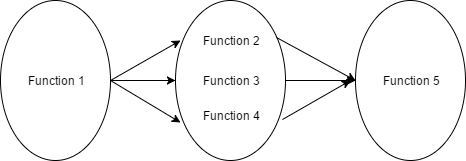
\includegraphics[scale=0.5]{functionalDependency.png}
\end{center}
\newpage

\SkipTocEntry\section{UML Diagrams}
\begin{figure}[h]
\begin{center}
\includegraphics[scale=0.5]{use_case.png}
\caption{Use Case Diagram}
\vspace{2cm}

\includegraphics[scale=0.5]{state.png}
\caption{State Diagram}
\end{center}
\end{figure}

\begin{figure}
\begin{center}
\includegraphics[scale=0.5]{activity.png}
\caption{Activity Diagram}

\vspace{1cm}
\includegraphics[scale=0.5]{sequence.png}
\caption{Sequence Diagram}
\end{center}
\end{figure}

\begin{figure}
\begin{center}
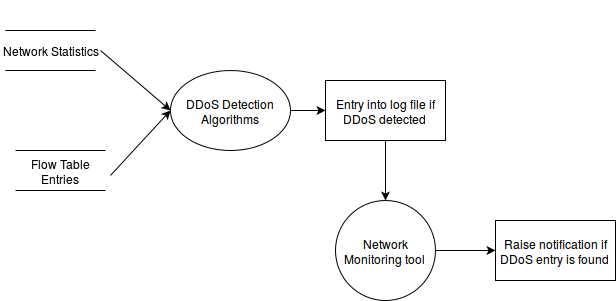
\includegraphics[scale=0.5]{dataflow0.png}
\caption{Dataflow Level 0 Diagram}

\vspace{3cm}
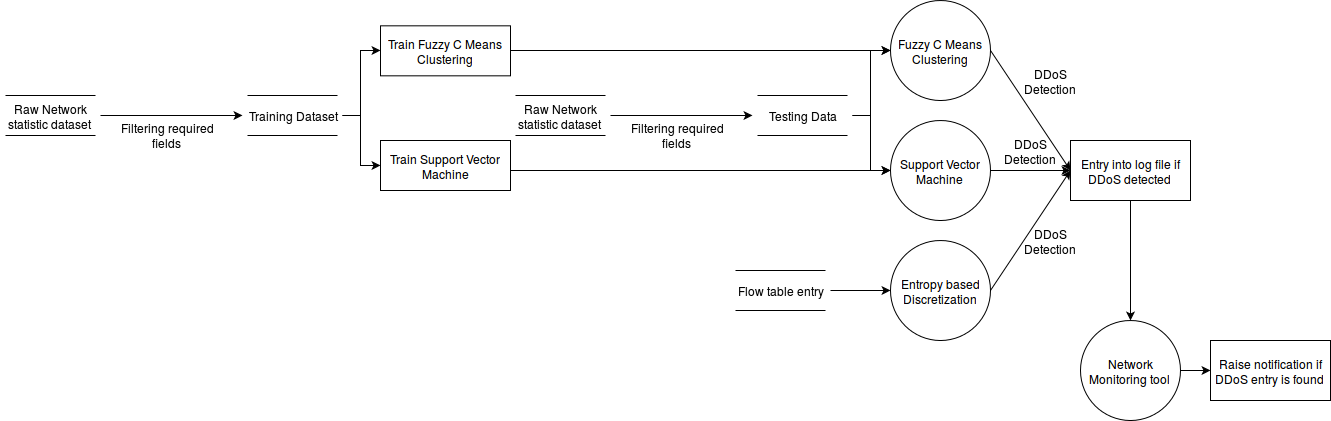
\includegraphics[scale=0.4]{dataflow1.png}
\caption{Dataflow Level 1 Diagram}
\end{center}
\end{figure}
\newpage

\AddToShipoutPictureBG*{%
\begin{tikzpicture}[overlay,remember picture]
\draw[line width=1.5pt]
    ($ (current page.north west) + (0.7cm,-0.7cm) $)
    rectangle
    ($ (current page.south east) + (-0.7cm,0.7cm) $);
\draw[line width=1.5pt]
    ($ (current page.north west) + (0.9cm,-0.9cm) $)
    rectangle
    ($ (current page.south east) + (-0.9cm,0.9cm) $);
\end{tikzpicture}
}
\SkipTocEntry\chapter{Annexure C}
\thispagestyle{empty}
\newpage
\SkipTocEntry\section{Project Planner - Figure}
\begin{figure}[h]
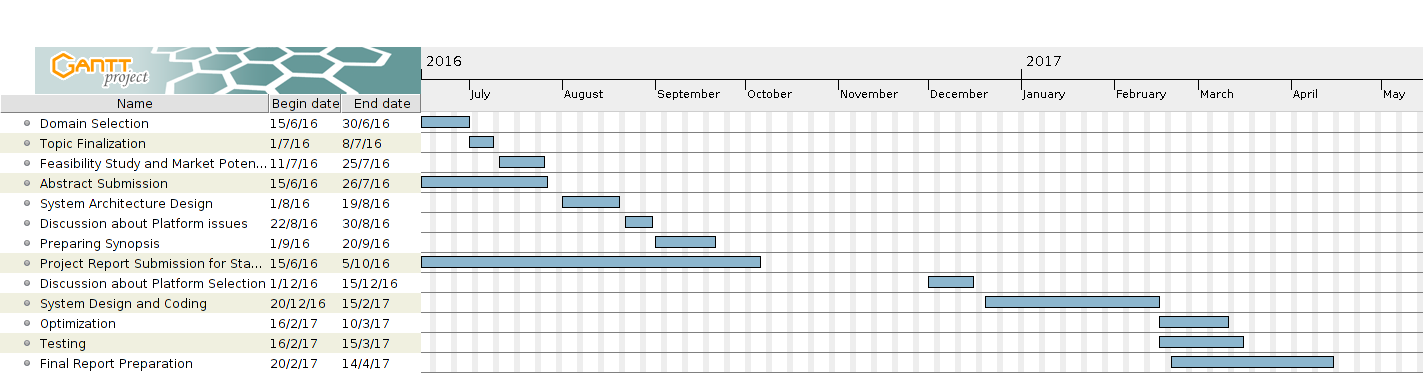
\includegraphics[width=18cm, height=8cm]{gantchart.png}
\caption{Gantt Chart}
\end{figure}

\SkipTocEntry\section{Project Planner - Table}
\begin{table}[h]
\begin{center}
\begin{tabular}{ |p{5cm}|p{3cm}|p{3cm}|p{1.5cm}| } 
 \hline
 \textbf{Name} & \textbf{Start Date} & \textbf{Due Date} & \textbf{Priority} \\ \hline
  Domain Selection & $15^{th}$ June 2016 & $30^{th}$ June 2016 & High \\ \hline
  Topic Finalization & $1^{st}$ July 2016 & $10^{th}$ July 2016 & High \\ \hline
  Feasibility Study and Market Potential Analysis & $11^{th}$ July 2016 & $25^{th}$ July 2016 & High \\ \hline
  Abstract Submission & - & $26^{th}$ July 2016 & Medium \\ \hline
  System Architecture Design & $1^{st}$ Aug 2016 & $20^{th}$ Aug 2016 & High \\ \hline    
  Discussion about Platform issues & $21^{st}$ Aug 2016 & $30^{th}$ Aug 2016 & High \\ \hline
  Preparing Synopsis & $1^{st}$ Sept 2016 & $20^{th}$ sept 2016 & High \\ \hline
  Project Report Submission for Stage I & - & $5^{th}$ Oct 2016 & Medium \\ \hline
  Discussion about Platform Selection & $1^{st}$ Dec. 2016 & $15^{th}$ Dec. 2016 & High \\ \hline
  System Design and Coding & $20^{th}$ Dec. 2016 & $15^{th}$ Feb. 2017 & High \\ \hline
  Testing & $16^{th}$ Feb. 2016 & $15^{th}$ Macrh 2016 & High \\ \hline
  Final Report Preparation & - & $15^{th}$ April 2016 & High \\ \hline
\end{tabular}
\end{center}
\caption{Project Planner}
\end{table}
\newpage

\AddToShipoutPictureBG*{%
\begin{tikzpicture}[overlay,remember picture]
\draw[line width=1.5pt]
    ($ (current page.north west) + (0.7cm,-0.7cm) $)
    rectangle
    ($ (current page.south east) + (-0.7cm,0.7cm) $);
\draw[line width=1.5pt]
    ($ (current page.north west) + (0.9cm,-0.9cm) $)
    rectangle
    ($ (current page.south east) + (-0.9cm,0.9cm) $);
\end{tikzpicture}
}
\SkipTocEntry\chapter{Annexure D}
\thispagestyle{empty}
\newpage
\SkipTocEntry\section{Reviewers Comments of Paper Submitted}
\begin{enumerate}
\item
\textbf{
Paper Title:
}

\item
\textbf{
Name of the Conference:
}

\item
\textbf{
Paper accepted/rejected:
}

\item
\textbf{
Review comments by reviewer:
}

\item
\textbf{
Corrective actions if any:
}
\end{enumerate}
\newpage

\AddToShipoutPictureBG*{%
\begin{tikzpicture}[overlay,remember picture]
\draw[line width=1.5pt]
    ($ (current page.north west) + (0.7cm,-0.7cm) $)
    rectangle
    ($ (current page.south east) + (-0.7cm,0.7cm) $);
\draw[line width=1.5pt]
    ($ (current page.north west) + (0.9cm,-0.9cm) $)
    rectangle
    ($ (current page.south east) + (-0.9cm,0.9cm) $);
\end{tikzpicture}
}
\SkipTocEntry\chapter{Annexure E}
\thispagestyle{empty}
\newpage
\SkipTocEntry\section{Plagiarism Report}

\newpage

\AddToShipoutPictureBG*{%
\begin{tikzpicture}[overlay,remember picture]
\draw[line width=1.5pt]
    ($ (current page.north west) + (0.7cm,-0.7cm) $)
    rectangle
    ($ (current page.south east) + (-0.7cm,0.7cm) $);
\draw[line width=1.5pt]
    ($ (current page.north west) + (0.9cm,-0.9cm) $)
    rectangle
    ($ (current page.south east) + (-0.9cm,0.9cm) $);
\end{tikzpicture}
}
\SkipTocEntry\chapter{Annexure F}
\thispagestyle{empty}
\newpage
\SkipTocEntry\section{Term II Project Laboratory Assignments}
\SkipTocEntry\subsection{Review of Design}
At the end of Term 1 assessment i.e. after completing the design phase of our project the reviews received were :
\begin{enumerate}
\item
To make sure high accuracy will be achieved.
\end{enumerate}

Taking into consideration this review, instead of using libraries for developing the algorithms, the algorithms have been developed right from scratch to mould them into models very specific to the use case of our project i.e. DDoS Detection.
\newline

Along with the feedback report of Term 1 assessment, we had also participated in the annual project competition PICT-Impetus and Concepts 2017, gaining valuable insights and reviews for our project. Industrial personnel belonging to companies like VmWare, Calsoft, Synerzip, ParallelMinds, Veritas, Cybage and many more. Having vast expertise in the domains of our project and were well versed with the latest technologies like SDN, ELK Stack, sFlow. Some of the criticism/feedbacks we received were :
\begin{enumerate}
\item
What kind of DDoS attacks are being detected?

\item
Why mitigation is not being included in the scope of the project?

\item
Change the controller used, from POX to OpenDayLight.

\item
Include adaptive learning module to adapt to the changing network scenarios. 
\end{enumerate}

Some crictics were encouraging and required our attention to be drawn to the issue, one such issue was including the adaptive module to varying network environments. Hence in entropy based discretization we have included the adaptive module which modifies the normal network entropy based on average weighted mean of previous 5 entries of normal entropy.
\newline

Positive feedback was also given stating the innovativeness of the project, inclusion of well known production based tools like ELK Stack, sFlow and replicating a real world environment. 
\newline
These feedbacks highlighted the strong and weak areas in our project which helped us a great deal in tackling the cross questions on the effectiveness of our project.

\SkipTocEntry\subsection{Project Installation and Setup}

\SkipTocEntry\subsection{Programming Interfaces}
The programming interfaces for SVM are:-
\begin{enumerate}
\item
\textbf{TShark} - It is network capturing and analysis tool which is used for capturing packet data from a live source, or from a previously captured network stream. It's native capturing file format is pcap format.
\item
\textbf{Numpy} - It is a python library which is used to perform mathematical operations over arrays.
\item
\textbf{Pandas} - It is a python library which is used for statistical data analysis, by performing batch operations rather than line by line operation.
\newpage
\item
\textbf{Flask} - Python micro web development framework.
\newline
Additional components :-
\begin{enumerate}
\item
Flask\_bootstrap

\item
Flask\_wtf

\item
Flask\_blueprint

\item
JQuery-3.0

\item
Flask\_sqlalchemy
\end{enumerate}
\end{enumerate}
\newpage

\AddToShipoutPictureBG*{%
\begin{tikzpicture}[overlay,remember picture]
\draw[line width=1.5pt]
    ($ (current page.north west) + (0.7cm,-0.7cm) $)
    rectangle
    ($ (current page.south east) + (-0.7cm,0.7cm) $);
\draw[line width=1.5pt]
    ($ (current page.north west) + (0.9cm,-0.9cm) $)
    rectangle
    ($ (current page.south east) + (-0.9cm,0.9cm) $);
\end{tikzpicture}
}
\SkipTocEntry\chapter{Annexure G}
\thispagestyle{empty}
\newpage
\SkipTocEntry\section{Information of Project Group Members}
\begin{flushright}
\includegraphics[width=60pt]{Achyuth.jpg}
\end{flushright}

\begin{enumerate}
\item Name : S. Achyuth Rao
\item Date of Birth : $19^{th}$ November, 1995
\item Gender : Male
\item Permanent Address : S-4, Mangalam apts., Tingre Nagar, Pune.
\item E-Mail : aachyutha2@gmail.com
\item Mobile/Contact No. : 07798845233
\item Placement Details : None
\item Paper Published : None

\end{enumerate}

\begin{flushright}
\includegraphics[width=60pt]{akib.jpg}
\end{flushright}

\begin{enumerate}
\item Name : Akib A. Shaikh
\item Date of Birth : $26^{th}$ April, 1996
\item Gender : Male
\item Permanent Address : 519, Centre Street, Camp, Pune.
\item E-Mail : akibshaikh117@gmail.com
\item Mobile/Contact No. : 09763851944
\item Placement Details : TCS Ltd.
\item Paper Published : None

\end{enumerate}
\newpage
\begin{flushright}
\includegraphics[width=60pt]{arun.jpg}
\end{flushright}

\begin{enumerate}
\item Name : Arun P. Pottekat
\item Date of Birth : $22^{nd}$ June, 1995
\item Gender : Male
\item Permanent Address : Citadel E/18, Ghorpadi, Pune.
\item E-Mail : apottekat@gmail.com		
\item Mobile/Contact No. : 09561120935
\item Placement Details : None
\item Paper Published : None

\end{enumerate}

\begin{flushright}
\includegraphics[width=60pt]{pranav.JPG}
\end{flushright}

\begin{enumerate}
\item Name : Pranav B. Tale
\item Date of Birth : $16^{th}$ June, 1995
\item Gender : Male
\item Permanent Address : 107-B, Rathi Nagar, Amravati, Maharashtra.
\item E-Mail : pranav.tale@gmail.com
\item Mobile/Contact No. : 09730692749
\item Placement Details : TCS Ltd.
\item Paper Published : None

\end{enumerate}
\end{document}